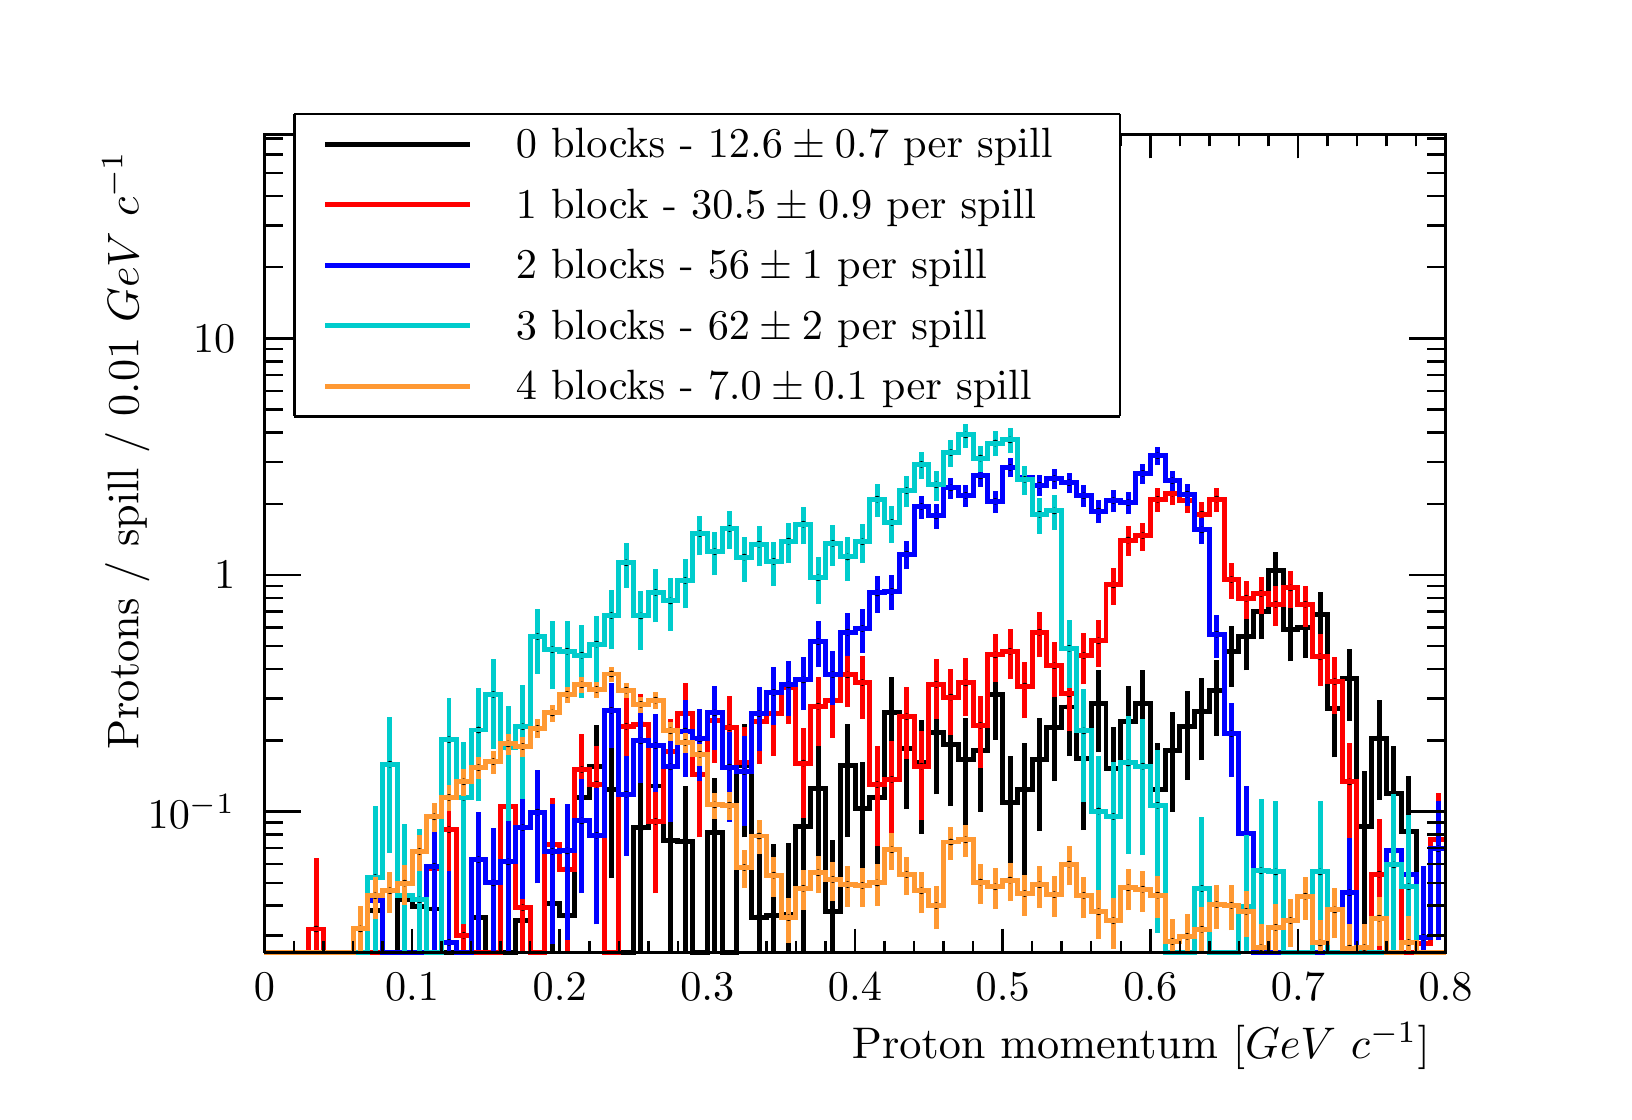
\begin{tikzpicture}
\pgfdeclareplotmark{cross} {
\pgfpathmoveto{\pgfpoint{-0.3\pgfplotmarksize}{\pgfplotmarksize}}
\pgfpathlineto{\pgfpoint{+0.3\pgfplotmarksize}{\pgfplotmarksize}}
\pgfpathlineto{\pgfpoint{+0.3\pgfplotmarksize}{0.3\pgfplotmarksize}}
\pgfpathlineto{\pgfpoint{+1\pgfplotmarksize}{0.3\pgfplotmarksize}}
\pgfpathlineto{\pgfpoint{+1\pgfplotmarksize}{-0.3\pgfplotmarksize}}
\pgfpathlineto{\pgfpoint{+0.3\pgfplotmarksize}{-0.3\pgfplotmarksize}}
\pgfpathlineto{\pgfpoint{+0.3\pgfplotmarksize}{-1.\pgfplotmarksize}}
\pgfpathlineto{\pgfpoint{-0.3\pgfplotmarksize}{-1.\pgfplotmarksize}}
\pgfpathlineto{\pgfpoint{-0.3\pgfplotmarksize}{-0.3\pgfplotmarksize}}
\pgfpathlineto{\pgfpoint{-1.\pgfplotmarksize}{-0.3\pgfplotmarksize}}
\pgfpathlineto{\pgfpoint{-1.\pgfplotmarksize}{0.3\pgfplotmarksize}}
\pgfpathlineto{\pgfpoint{-0.3\pgfplotmarksize}{0.3\pgfplotmarksize}}
\pgfpathclose
\pgfusepathqstroke
}
\pgfdeclareplotmark{cross*} {
\pgfpathmoveto{\pgfpoint{-0.3\pgfplotmarksize}{\pgfplotmarksize}}
\pgfpathlineto{\pgfpoint{+0.3\pgfplotmarksize}{\pgfplotmarksize}}
\pgfpathlineto{\pgfpoint{+0.3\pgfplotmarksize}{0.3\pgfplotmarksize}}
\pgfpathlineto{\pgfpoint{+1\pgfplotmarksize}{0.3\pgfplotmarksize}}
\pgfpathlineto{\pgfpoint{+1\pgfplotmarksize}{-0.3\pgfplotmarksize}}
\pgfpathlineto{\pgfpoint{+0.3\pgfplotmarksize}{-0.3\pgfplotmarksize}}
\pgfpathlineto{\pgfpoint{+0.3\pgfplotmarksize}{-1.\pgfplotmarksize}}
\pgfpathlineto{\pgfpoint{-0.3\pgfplotmarksize}{-1.\pgfplotmarksize}}
\pgfpathlineto{\pgfpoint{-0.3\pgfplotmarksize}{-0.3\pgfplotmarksize}}
\pgfpathlineto{\pgfpoint{-1.\pgfplotmarksize}{-0.3\pgfplotmarksize}}
\pgfpathlineto{\pgfpoint{-1.\pgfplotmarksize}{0.3\pgfplotmarksize}}
\pgfpathlineto{\pgfpoint{-0.3\pgfplotmarksize}{0.3\pgfplotmarksize}}
\pgfpathclose
\pgfusepathqfillstroke
}
\pgfdeclareplotmark{newstar} {
\pgfpathmoveto{\pgfqpoint{0pt}{\pgfplotmarksize}}
\pgfpathlineto{\pgfqpointpolar{44}{0.5\pgfplotmarksize}}
\pgfpathlineto{\pgfqpointpolar{18}{\pgfplotmarksize}}
\pgfpathlineto{\pgfqpointpolar{-20}{0.5\pgfplotmarksize}}
\pgfpathlineto{\pgfqpointpolar{-54}{\pgfplotmarksize}}
\pgfpathlineto{\pgfqpointpolar{-90}{0.5\pgfplotmarksize}}
\pgfpathlineto{\pgfqpointpolar{234}{\pgfplotmarksize}}
\pgfpathlineto{\pgfqpointpolar{198}{0.5\pgfplotmarksize}}
\pgfpathlineto{\pgfqpointpolar{162}{\pgfplotmarksize}}
\pgfpathlineto{\pgfqpointpolar{134}{0.5\pgfplotmarksize}}
\pgfpathclose
\pgfusepathqstroke
}
\pgfdeclareplotmark{newstar*} {
\pgfpathmoveto{\pgfqpoint{0pt}{\pgfplotmarksize}}
\pgfpathlineto{\pgfqpointpolar{44}{0.5\pgfplotmarksize}}
\pgfpathlineto{\pgfqpointpolar{18}{\pgfplotmarksize}}
\pgfpathlineto{\pgfqpointpolar{-20}{0.5\pgfplotmarksize}}
\pgfpathlineto{\pgfqpointpolar{-54}{\pgfplotmarksize}}
\pgfpathlineto{\pgfqpointpolar{-90}{0.5\pgfplotmarksize}}
\pgfpathlineto{\pgfqpointpolar{234}{\pgfplotmarksize}}
\pgfpathlineto{\pgfqpointpolar{198}{0.5\pgfplotmarksize}}
\pgfpathlineto{\pgfqpointpolar{162}{\pgfplotmarksize}}
\pgfpathlineto{\pgfqpointpolar{134}{0.5\pgfplotmarksize}}
\pgfpathclose
\pgfusepathqfillstroke
}
\definecolor{c}{rgb}{1,1,1};
\draw [color=c, fill=c] (0,0) rectangle (20,13.4957);
\draw [color=c, fill=c] (3,1.75444) rectangle (18,12.1461);
\definecolor{c}{rgb}{0,0,0};
\draw [c,line width=0.9] (3,1.75444) -- (3,12.1461) -- (18,12.1461) -- (18,1.75444) -- (3,1.75444);
\definecolor{c}{rgb}{1,1,1};
\draw [color=c, fill=c] (3,1.75444) rectangle (18,12.1461);
\definecolor{c}{rgb}{0,0,0};
\draw [c,line width=0.9] (3,1.75444) -- (3,12.1461) -- (18,12.1461) -- (18,1.75444) -- (3,1.75444);
\draw [c,line width=0.9] (3,1.75444) -- (3.1875,1.75444) -- (3.1875,1.75444) -- (3.375,1.75444) -- (3.375,1.75444) -- (3.5625,1.75444) -- (3.5625,1.75444) -- (3.75,1.75444) -- (3.75,1.75444) -- (3.9375,1.75444) -- (3.9375,1.75444) -- (4.125,1.75444)
 -- (4.125,1.75444) -- (4.3125,1.75444) -- (4.3125,1.75444) -- (4.5,1.75444) -- (4.5,1.75444) -- (4.6875,1.75444) -- (4.6875,1.75444) -- (4.875,1.75444) -- (4.875,1.75444) -- (5.0625,1.75444) -- (5.0625,1.75444) -- (5.25,1.75444) -- (5.25,1.75444) --
 (5.4375,1.75444) -- (5.4375,1.75444) -- (5.625,1.75444) -- (5.625,1.75444) -- (5.8125,1.75444) -- (5.8125,1.75444) -- (6,1.75444) -- (6,1.75444) -- (6.1875,1.75444) -- (6.1875,1.75444) -- (6.375,1.75444) -- (6.375,1.75444) -- (6.5625,1.75444) --
 (6.5625,1.75444) -- (6.75,1.75444) -- (6.75,1.75444) -- (6.9375,1.75444) -- (6.9375,1.75444) -- (7.125,1.75444) -- (7.125,1.75444) -- (7.3125,1.75444) -- (7.3125,1.75444) -- (7.5,1.75444) -- (7.5,1.75444) -- (7.6875,1.75444) -- (7.6875,1.75444) --
 (7.875,1.75444) -- (7.875,1.75444) -- (8.0625,1.75444) -- (8.0625,1.75444) -- (8.25,1.75444) -- (8.25,1.75444) -- (8.4375,1.75444) -- (8.4375,1.75444) -- (8.625,1.75444) -- (8.625,1.75444) -- (8.8125,1.75444) -- (8.8125,1.75444) -- (9,1.75444) --
 (9,1.75444) -- (9.1875,1.75444) -- (9.1875,1.75444) -- (9.375,1.75444) -- (9.375,1.75444) -- (9.5625,1.75444) -- (9.5625,1.75444) -- (9.75,1.75444) -- (9.75,1.75444) -- (9.9375,1.75444) -- (9.9375,1.75444) -- (10.125,1.75444) -- (10.125,1.75444) --
 (10.3125,1.75444) -- (10.3125,1.75444) -- (10.5,1.75444) -- (10.5,1.75444) -- (10.6875,1.75444) -- (10.6875,1.75444) -- (10.875,1.75444) -- (10.875,1.75444) -- (11.0625,1.75444) -- (11.0625,1.75444) -- (11.25,1.75444) -- (11.25,1.75444) --
 (11.4375,1.75444) -- (11.4375,1.75444) -- (11.625,1.75444) -- (11.625,1.75444) -- (11.8125,1.75444) -- (11.8125,1.75444) -- (12,1.75444) -- (12,1.75444) -- (12.1875,1.75444) -- (12.1875,1.75444) -- (12.375,1.75444) -- (12.375,1.75444) --
 (12.5625,1.75444) -- (12.5625,1.75444) -- (12.75,1.75444) -- (12.75,1.75444) -- (12.9375,1.75444) -- (12.9375,1.75444) -- (13.125,1.75444) -- (13.125,1.75444) -- (13.3125,1.75444) -- (13.3125,1.75444) -- (13.5,1.75444) -- (13.5,1.75444) --
 (13.6875,1.75444) -- (13.6875,1.75444) -- (13.875,1.75444) -- (13.875,1.75444) -- (14.0625,1.75444) -- (14.0625,1.75444) -- (14.25,1.75444) -- (14.25,1.75444) -- (14.4375,1.75444) -- (14.4375,1.75444) -- (14.625,1.75444) -- (14.625,1.75444) --
 (14.8125,1.75444) -- (14.8125,1.75444) -- (15,1.75444) -- (15,1.75444) -- (15.1875,1.75444) -- (15.1875,1.75444) -- (15.375,1.75444) -- (15.375,1.75444) -- (15.5625,1.75444) -- (15.5625,1.75444) -- (15.75,1.75444) -- (15.75,1.75444) --
 (15.9375,1.75444) -- (15.9375,1.75444) -- (16.125,1.75444) -- (16.125,1.75444) -- (16.3125,1.75444) -- (16.3125,1.75444) -- (16.5,1.75444) -- (16.5,1.75444) -- (16.6875,1.75444) -- (16.6875,1.75444) -- (16.875,1.75444) -- (16.875,1.75444) --
 (17.0625,1.75444) -- (17.0625,1.75444) -- (17.25,1.75444) -- (17.25,1.75444) -- (17.4375,1.75444) -- (17.4375,1.75444) -- (17.625,1.75444) -- (17.625,1.75444) -- (17.8125,1.75444) -- (17.8125,1.75444) -- (18,1.75444);
\draw [c,line width=0.9] (3,1.75444) -- (18,1.75444);
\draw [c,line width=0.9] (3,2.05809) -- (3,1.75444);
\draw [c,line width=0.9] (3.375,1.90627) -- (3.375,1.75444);
\draw [c,line width=0.9] (3.75,1.90627) -- (3.75,1.75444);
\draw [c,line width=0.9] (4.125,1.90627) -- (4.125,1.75444);
\draw [c,line width=0.9] (4.5,1.90627) -- (4.5,1.75444);
\draw [c,line width=0.9] (4.875,2.05809) -- (4.875,1.75444);
\draw [c,line width=0.9] (5.25,1.90627) -- (5.25,1.75444);
\draw [c,line width=0.9] (5.625,1.90627) -- (5.625,1.75444);
\draw [c,line width=0.9] (6,1.90627) -- (6,1.75444);
\draw [c,line width=0.9] (6.375,1.90627) -- (6.375,1.75444);
\draw [c,line width=0.9] (6.75,2.05809) -- (6.75,1.75444);
\draw [c,line width=0.9] (7.125,1.90627) -- (7.125,1.75444);
\draw [c,line width=0.9] (7.5,1.90627) -- (7.5,1.75444);
\draw [c,line width=0.9] (7.875,1.90627) -- (7.875,1.75444);
\draw [c,line width=0.9] (8.25,1.90627) -- (8.25,1.75444);
\draw [c,line width=0.9] (8.625,2.05809) -- (8.625,1.75444);
\draw [c,line width=0.9] (9,1.90627) -- (9,1.75444);
\draw [c,line width=0.9] (9.375,1.90627) -- (9.375,1.75444);
\draw [c,line width=0.9] (9.75,1.90627) -- (9.75,1.75444);
\draw [c,line width=0.9] (10.125,1.90627) -- (10.125,1.75444);
\draw [c,line width=0.9] (10.5,2.05809) -- (10.5,1.75444);
\draw [c,line width=0.9] (10.875,1.90627) -- (10.875,1.75444);
\draw [c,line width=0.9] (11.25,1.90627) -- (11.25,1.75444);
\draw [c,line width=0.9] (11.625,1.90627) -- (11.625,1.75444);
\draw [c,line width=0.9] (12,1.90627) -- (12,1.75444);
\draw [c,line width=0.9] (12.375,2.05809) -- (12.375,1.75444);
\draw [c,line width=0.9] (12.75,1.90627) -- (12.75,1.75444);
\draw [c,line width=0.9] (13.125,1.90627) -- (13.125,1.75444);
\draw [c,line width=0.9] (13.5,1.90627) -- (13.5,1.75444);
\draw [c,line width=0.9] (13.875,1.90627) -- (13.875,1.75444);
\draw [c,line width=0.9] (14.25,2.05809) -- (14.25,1.75444);
\draw [c,line width=0.9] (14.625,1.90627) -- (14.625,1.75444);
\draw [c,line width=0.9] (15,1.90627) -- (15,1.75444);
\draw [c,line width=0.9] (15.375,1.90627) -- (15.375,1.75444);
\draw [c,line width=0.9] (15.75,1.90627) -- (15.75,1.75444);
\draw [c,line width=0.9] (16.125,2.05809) -- (16.125,1.75444);
\draw [c,line width=0.9] (16.5,1.90627) -- (16.5,1.75444);
\draw [c,line width=0.9] (16.875,1.90627) -- (16.875,1.75444);
\draw [c,line width=0.9] (17.25,1.90627) -- (17.25,1.75444);
\draw [c,line width=0.9] (17.625,1.90627) -- (17.625,1.75444);
\draw [c,line width=0.9] (18,2.05809) -- (18,1.75444);
\draw [anchor=base] (3,1.14713) node[scale=1.52731, color=c, rotate=0]{0};
\draw [anchor=base] (4.875,1.14713) node[scale=1.52731, color=c, rotate=0]{0.1};
\draw [anchor=base] (6.75,1.14713) node[scale=1.52731, color=c, rotate=0]{0.2};
\draw [anchor=base] (8.625,1.14713) node[scale=1.52731, color=c, rotate=0]{0.3};
\draw [anchor=base] (10.5,1.14713) node[scale=1.52731, color=c, rotate=0]{0.4};
\draw [anchor=base] (12.375,1.14713) node[scale=1.52731, color=c, rotate=0]{0.5};
\draw [anchor=base] (14.25,1.14713) node[scale=1.52731, color=c, rotate=0]{0.6};
\draw [anchor=base] (16.125,1.14713) node[scale=1.52731, color=c, rotate=0]{0.7};
\draw [anchor=base] (18,1.14713) node[scale=1.52731, color=c, rotate=0]{0.8};
\draw [anchor= east] (18,0.566819) node[scale=1.6, color=c, rotate=0]{Proton momentum [$\text{GeV}~c^{-1}$]};
\draw [c,line width=0.9] (3,12.1461) -- (18,12.1461);
\draw [c,line width=0.9] (3,11.8425) -- (3,12.1461);
\draw [c,line width=0.9] (3.375,11.9943) -- (3.375,12.1461);
\draw [c,line width=0.9] (3.75,11.9943) -- (3.75,12.1461);
\draw [c,line width=0.9] (4.125,11.9943) -- (4.125,12.1461);
\draw [c,line width=0.9] (4.5,11.9943) -- (4.5,12.1461);
\draw [c,line width=0.9] (4.875,11.8425) -- (4.875,12.1461);
\draw [c,line width=0.9] (5.25,11.9943) -- (5.25,12.1461);
\draw [c,line width=0.9] (5.625,11.9943) -- (5.625,12.1461);
\draw [c,line width=0.9] (6,11.9943) -- (6,12.1461);
\draw [c,line width=0.9] (6.375,11.9943) -- (6.375,12.1461);
\draw [c,line width=0.9] (6.75,11.8425) -- (6.75,12.1461);
\draw [c,line width=0.9] (7.125,11.9943) -- (7.125,12.1461);
\draw [c,line width=0.9] (7.5,11.9943) -- (7.5,12.1461);
\draw [c,line width=0.9] (7.875,11.9943) -- (7.875,12.1461);
\draw [c,line width=0.9] (8.25,11.9943) -- (8.25,12.1461);
\draw [c,line width=0.9] (8.625,11.8425) -- (8.625,12.1461);
\draw [c,line width=0.9] (9,11.9943) -- (9,12.1461);
\draw [c,line width=0.9] (9.375,11.9943) -- (9.375,12.1461);
\draw [c,line width=0.9] (9.75,11.9943) -- (9.75,12.1461);
\draw [c,line width=0.9] (10.125,11.9943) -- (10.125,12.1461);
\draw [c,line width=0.9] (10.5,11.8425) -- (10.5,12.1461);
\draw [c,line width=0.9] (10.875,11.9943) -- (10.875,12.1461);
\draw [c,line width=0.9] (11.25,11.9943) -- (11.25,12.1461);
\draw [c,line width=0.9] (11.625,11.9943) -- (11.625,12.1461);
\draw [c,line width=0.9] (12,11.9943) -- (12,12.1461);
\draw [c,line width=0.9] (12.375,11.8425) -- (12.375,12.1461);
\draw [c,line width=0.9] (12.75,11.9943) -- (12.75,12.1461);
\draw [c,line width=0.9] (13.125,11.9943) -- (13.125,12.1461);
\draw [c,line width=0.9] (13.5,11.9943) -- (13.5,12.1461);
\draw [c,line width=0.9] (13.875,11.9943) -- (13.875,12.1461);
\draw [c,line width=0.9] (14.25,11.8425) -- (14.25,12.1461);
\draw [c,line width=0.9] (14.625,11.9943) -- (14.625,12.1461);
\draw [c,line width=0.9] (15,11.9943) -- (15,12.1461);
\draw [c,line width=0.9] (15.375,11.9943) -- (15.375,12.1461);
\draw [c,line width=0.9] (15.75,11.9943) -- (15.75,12.1461);
\draw [c,line width=0.9] (16.125,11.8425) -- (16.125,12.1461);
\draw [c,line width=0.9] (16.5,11.9943) -- (16.5,12.1461);
\draw [c,line width=0.9] (16.875,11.9943) -- (16.875,12.1461);
\draw [c,line width=0.9] (17.25,11.9943) -- (17.25,12.1461);
\draw [c,line width=0.9] (17.625,11.9943) -- (17.625,12.1461);
\draw [c,line width=0.9] (18,11.8425) -- (18,12.1461);
\draw [c,line width=0.9] (3,1.75444) -- (3,12.1461);
\draw [c,line width=0.9] (3.231,1.97632) -- (3,1.97632);
\draw [c,line width=0.9] (3.231,2.35171) -- (3,2.35171);
\draw [c,line width=0.9] (3.231,2.64288) -- (3,2.64288);
\draw [c,line width=0.9] (3.231,2.88079) -- (3,2.88079);
\draw [c,line width=0.9] (3.231,3.08193) -- (3,3.08193);
\draw [c,line width=0.9] (3.231,3.25618) -- (3,3.25618);
\draw [c,line width=0.9] (3.231,3.40987) -- (3,3.40987);
\draw [c,line width=0.9] (3.462,3.54735) -- (3,3.54735);
\draw [anchor= east] (2.82,3.54735) node[scale=1.52731, color=c, rotate=0]{$10^{-1}$};
\draw [c,line width=0.9] (3.231,4.45182) -- (3,4.45182);
\draw [c,line width=0.9] (3.231,4.9809) -- (3,4.9809);
\draw [c,line width=0.9] (3.231,5.35629) -- (3,5.35629);
\draw [c,line width=0.9] (3.231,5.64747) -- (3,5.64747);
\draw [c,line width=0.9] (3.231,5.88537) -- (3,5.88537);
\draw [c,line width=0.9] (3.231,6.08652) -- (3,6.08652);
\draw [c,line width=0.9] (3.231,6.26076) -- (3,6.26076);
\draw [c,line width=0.9] (3.231,6.41445) -- (3,6.41445);
\draw [c,line width=0.9] (3.462,6.55194) -- (3,6.55194);
\draw [anchor= east] (2.82,6.55194) node[scale=1.52731, color=c, rotate=0]{1};
\draw [c,line width=0.9] (3.231,7.45641) -- (3,7.45641);
\draw [c,line width=0.9] (3.231,7.98549) -- (3,7.98549);
\draw [c,line width=0.9] (3.231,8.36088) -- (3,8.36088);
\draw [c,line width=0.9] (3.231,8.65205) -- (3,8.65205);
\draw [c,line width=0.9] (3.231,8.88996) -- (3,8.88996);
\draw [c,line width=0.9] (3.231,9.0911) -- (3,9.0911);
\draw [c,line width=0.9] (3.231,9.26535) -- (3,9.26535);
\draw [c,line width=0.9] (3.231,9.41904) -- (3,9.41904);
\draw [c,line width=0.9] (3.462,9.55652) -- (3,9.55652);
\draw [anchor= east] (2.82,9.55652) node[scale=1.52731, color=c, rotate=0]{10};
\draw [c,line width=0.9] (3.231,10.461) -- (3,10.461);
\draw [c,line width=0.9] (3.231,10.9901) -- (3,10.9901);
\draw [c,line width=0.9] (3.231,11.3655) -- (3,11.3655);
\draw [c,line width=0.9] (3.231,11.6566) -- (3,11.6566);
\draw [c,line width=0.9] (3.231,11.8945) -- (3,11.8945);
\draw [c,line width=0.9] (3.231,12.0957) -- (3,12.0957);
\draw [anchor= east] (1.24,12.1461) node[scale=1.6, color=c, rotate=90]{Protons / spill / $0.01~\text{GeV}~c^{-1}$};
\draw [c,line width=0.9] (18,1.75444) -- (18,12.1461);
\draw [c,line width=0.9] (17.769,1.97632) -- (18,1.97632);
\draw [c,line width=0.9] (17.769,2.35171) -- (18,2.35171);
\draw [c,line width=0.9] (17.769,2.64288) -- (18,2.64288);
\draw [c,line width=0.9] (17.769,2.88079) -- (18,2.88079);
\draw [c,line width=0.9] (17.769,3.08193) -- (18,3.08193);
\draw [c,line width=0.9] (17.769,3.25618) -- (18,3.25618);
\draw [c,line width=0.9] (17.769,3.40987) -- (18,3.40987);
\draw [c,line width=0.9] (17.538,3.54735) -- (18,3.54735);
\draw [c,line width=0.9] (17.769,4.45182) -- (18,4.45182);
\draw [c,line width=0.9] (17.769,4.9809) -- (18,4.9809);
\draw [c,line width=0.9] (17.769,5.35629) -- (18,5.35629);
\draw [c,line width=0.9] (17.769,5.64747) -- (18,5.64747);
\draw [c,line width=0.9] (17.769,5.88537) -- (18,5.88537);
\draw [c,line width=0.9] (17.769,6.08652) -- (18,6.08652);
\draw [c,line width=0.9] (17.769,6.26076) -- (18,6.26076);
\draw [c,line width=0.9] (17.769,6.41445) -- (18,6.41445);
\draw [c,line width=0.9] (17.538,6.55194) -- (18,6.55194);
\draw [c,line width=0.9] (17.769,7.45641) -- (18,7.45641);
\draw [c,line width=0.9] (17.769,7.98549) -- (18,7.98549);
\draw [c,line width=0.9] (17.769,8.36088) -- (18,8.36088);
\draw [c,line width=0.9] (17.769,8.65205) -- (18,8.65205);
\draw [c,line width=0.9] (17.769,8.88996) -- (18,8.88996);
\draw [c,line width=0.9] (17.769,9.0911) -- (18,9.0911);
\draw [c,line width=0.9] (17.769,9.26535) -- (18,9.26535);
\draw [c,line width=0.9] (17.769,9.41904) -- (18,9.41904);
\draw [c,line width=0.9] (17.538,9.55652) -- (18,9.55652);
\draw [c,line width=0.9] (17.769,10.461) -- (18,10.461);
\draw [c,line width=0.9] (17.769,10.9901) -- (18,10.9901);
\draw [c,line width=0.9] (17.769,11.3655) -- (18,11.3655);
\draw [c,line width=0.9] (17.769,11.6566) -- (18,11.6566);
\draw [c,line width=0.9] (17.769,11.8945) -- (18,11.8945);
\draw [c,line width=0.9] (17.769,12.0957) -- (18,12.0957);
\draw [c,line width=1.8] (4.40625,1.75444) -- (4.40625,2.28698);
\draw [c,line width=1.8] (4.40625,2.28698) -- (4.40625,3.19146);
\foreach \P in {(4.40625,2.28698)}{\draw[mark options={color=c,fill=c},mark size=2.402402pt,mark=*,mark size=1pt] plot coordinates {\P};}
\draw [c,line width=1.8] (4.78125,1.75444) -- (4.78125,2.42605);
\draw [c,line width=1.8] (4.78125,2.42605) -- (4.78125,3.33052);
\foreach \P in {(4.78125,2.42605)}{\draw[mark options={color=c,fill=c},mark size=2.402402pt,mark=*,mark size=1pt] plot coordinates {\P};}
\draw [c,line width=1.8] (4.96875,1.75444) -- (4.96875,2.3475);
\draw [c,line width=1.8] (4.96875,2.3475) -- (4.96875,3.25197);
\foreach \P in {(4.96875,2.3475)}{\draw[mark options={color=c,fill=c},mark size=2.402402pt,mark=*,mark size=1pt] plot coordinates {\P};}
\draw [c,line width=1.8] (5.15625,1.75444) -- (5.15625,2.30993);
\draw [c,line width=1.8] (5.15625,2.30993) -- (5.15625,3.2144);
\foreach \P in {(5.15625,2.30993)}{\draw[mark options={color=c,fill=c},mark size=2.402402pt,mark=*,mark size=1pt] plot coordinates {\P};}
\draw [c,line width=1.8] (5.71875,1.75444) -- (5.71875,2.20757);
\draw [c,line width=1.8] (5.71875,2.20757) -- (5.71875,3.11204);
\foreach \P in {(5.71875,2.20757)}{\draw[mark options={color=c,fill=c},mark size=2.402402pt,mark=*,mark size=1pt] plot coordinates {\P};}
\draw [c,line width=1.8] (6.28125,1.75444) -- (6.28125,2.16546);
\draw [c,line width=1.8] (6.28125,2.16546) -- (6.28125,3.06993);
\foreach \P in {(6.28125,2.16546)}{\draw[mark options={color=c,fill=c},mark size=2.402402pt,mark=*,mark size=1pt] plot coordinates {\P};}
\draw [c,line width=1.8] (6.65625,1.75444) -- (6.65625,2.37641);
\draw [c,line width=1.8] (6.65625,2.37641) -- (6.65625,3.28088);
\foreach \P in {(6.65625,2.37641)}{\draw[mark options={color=c,fill=c},mark size=2.402402pt,mark=*,mark size=1pt] plot coordinates {\P};}
\draw [c,line width=1.8] (6.84375,1.75444) -- (6.84375,2.22481);
\draw [c,line width=1.8] (6.84375,2.22481) -- (6.84375,3.12928);
\foreach \P in {(6.84375,2.22481)}{\draw[mark options={color=c,fill=c},mark size=2.402402pt,mark=*,mark size=1pt] plot coordinates {\P};}
\draw [c,line width=1.8] (7.03125,2.60297) -- (7.03125,3.72702);
\draw [c,line width=1.8] (7.03125,3.72702) -- (7.03125,4.32178);
\foreach \P in {(7.03125,3.72702)}{\draw[mark options={color=c,fill=c},mark size=2.402402pt,mark=*,mark size=1pt] plot coordinates {\P};}
\draw [c,line width=1.8] (7.21875,3.21113) -- (7.21875,4.11788);
\draw [c,line width=1.8] (7.21875,4.11788) -- (7.21875,4.64772);
\foreach \P in {(7.21875,4.11788)}{\draw[mark options={color=c,fill=c},mark size=2.402402pt,mark=*,mark size=1pt] plot coordinates {\P};}
\draw [c,line width=1.8] (7.40625,2.69856) -- (7.40625,3.82434);
\draw [c,line width=1.8] (7.40625,3.82434) -- (7.40625,4.41957);
\foreach \P in {(7.40625,3.82434)}{\draw[mark options={color=c,fill=c},mark size=2.402402pt,mark=*,mark size=1pt] plot coordinates {\P};}
\draw [c,line width=1.8] (7.78125,1.75444) -- (7.78125,3.3418);
\draw [c,line width=1.8] (7.78125,3.3418) -- (7.78125,4.04248);
\foreach \P in {(7.78125,3.3418)}{\draw[mark options={color=c,fill=c},mark size=2.402402pt,mark=*,mark size=1pt] plot coordinates {\P};}
\draw [c,line width=1.8] (7.96875,2.73321) -- (7.96875,3.872);
\draw [c,line width=1.8] (7.96875,3.872) -- (7.96875,4.47069);
\foreach \P in {(7.96875,3.872)}{\draw[mark options={color=c,fill=c},mark size=2.402402pt,mark=*,mark size=1pt] plot coordinates {\P};}
\draw [c,line width=1.8] (8.15625,1.75444) -- (8.15625,3.18032);
\draw [c,line width=1.8] (8.15625,3.18032) -- (8.15625,3.87821);
\foreach \P in {(8.15625,3.18032)}{\draw[mark options={color=c,fill=c},mark size=2.402402pt,mark=*,mark size=1pt] plot coordinates {\P};}
\draw [c,line width=1.8] (8.34375,1.75444) -- (8.34375,3.17248);
\draw [c,line width=1.8] (8.34375,3.17248) -- (8.34375,3.87645);
\foreach \P in {(8.34375,3.17248)}{\draw[mark options={color=c,fill=c},mark size=2.402402pt,mark=*,mark size=1pt] plot coordinates {\P};}
\draw [c,line width=1.8] (8.71875,1.75444) -- (8.71875,3.27907);
\draw [c,line width=1.8] (8.71875,3.27907) -- (8.71875,3.97755);
\foreach \P in {(8.71875,3.27907)}{\draw[mark options={color=c,fill=c},mark size=2.402402pt,mark=*,mark size=1pt] plot coordinates {\P};}
\draw [c,line width=1.8] (9.09375,3.21939) -- (9.09375,4.13038);
\draw [c,line width=1.8] (9.09375,4.13038) -- (9.09375,4.66163);
\foreach \P in {(9.09375,4.13038)}{\draw[mark options={color=c,fill=c},mark size=2.402402pt,mark=*,mark size=1pt] plot coordinates {\P};}
\draw [c,line width=1.8] (9.28125,1.75444) -- (9.28125,2.20757);
\draw [c,line width=1.8] (9.28125,2.20757) -- (9.28125,3.11204);
\foreach \P in {(9.28125,2.20757)}{\draw[mark options={color=c,fill=c},mark size=2.402402pt,mark=*,mark size=1pt] plot coordinates {\P};}
\draw [c,line width=1.8] (9.46875,1.75444) -- (9.46875,2.22481);
\draw [c,line width=1.8] (9.46875,2.22481) -- (9.46875,3.12928);
\foreach \P in {(9.46875,2.22481)}{\draw[mark options={color=c,fill=c},mark size=2.402402pt,mark=*,mark size=1pt] plot coordinates {\P};}
\draw [c,line width=1.8] (9.65625,1.75444) -- (9.65625,2.24227);
\draw [c,line width=1.8] (9.65625,2.24227) -- (9.65625,3.14674);
\foreach \P in {(9.65625,2.24227)}{\draw[mark options={color=c,fill=c},mark size=2.402402pt,mark=*,mark size=1pt] plot coordinates {\P};}
\draw [c,line width=1.8] (9.84375,1.75444) -- (9.84375,3.35866);
\draw [c,line width=1.8] (9.84375,3.35866) -- (9.84375,4.0657);
\foreach \P in {(9.84375,3.35866)}{\draw[mark options={color=c,fill=c},mark size=2.402402pt,mark=*,mark size=1pt] plot coordinates {\P};}
\draw [c,line width=1.8] (10.0312,2.6947) -- (10.0312,3.83827);
\draw [c,line width=1.8] (10.0312,3.83827) -- (10.0312,4.43822);
\foreach \P in {(10.0312,3.83827)}{\draw[mark options={color=c,fill=c},mark size=2.402402pt,mark=*,mark size=1pt] plot coordinates {\P};}
\draw [c,line width=1.8] (10.2188,1.75444) -- (10.2188,2.27792);
\draw [c,line width=1.8] (10.2188,2.27792) -- (10.2188,3.18239);
\foreach \P in {(10.2188,2.27792)}{\draw[mark options={color=c,fill=c},mark size=2.402402pt,mark=*,mark size=1pt] plot coordinates {\P};}
\draw [c,line width=1.8] (10.4062,3.22404) -- (10.4062,4.12993);
\draw [c,line width=1.8] (10.4062,4.12993) -- (10.4062,4.65949);
\foreach \P in {(10.4062,4.12993)}{\draw[mark options={color=c,fill=c},mark size=2.402402pt,mark=*,mark size=1pt] plot coordinates {\P};}
\draw [c,line width=1.8] (10.5938,2.46038) -- (10.5938,3.58472);
\draw [c,line width=1.8] (10.5938,3.58472) -- (10.5938,4.17956);
\foreach \P in {(10.5938,3.58472)}{\draw[mark options={color=c,fill=c},mark size=2.402402pt,mark=*,mark size=1pt] plot coordinates {\P};}
\draw [c,line width=1.8] (10.7812,2.60346) -- (10.7812,3.72846);
\draw [c,line width=1.8] (10.7812,3.72846) -- (10.7812,4.32348);
\foreach \P in {(10.7812,3.72846)}{\draw[mark options={color=c,fill=c},mark size=2.402402pt,mark=*,mark size=1pt] plot coordinates {\P};}
\draw [c,line width=1.8] (10.9688,4.11312) -- (10.9688,4.80344);
\draw [c,line width=1.8] (10.9688,4.80344) -- (10.9688,5.25255);
\foreach \P in {(10.9688,4.80344)}{\draw[mark options={color=c,fill=c},mark size=2.402402pt,mark=*,mark size=1pt] plot coordinates {\P};}
\draw [c,line width=1.8] (11.1562,3.57618) -- (11.1562,4.35236);
\draw [c,line width=1.8] (11.1562,4.35236) -- (11.1562,4.83572);
\foreach \P in {(11.1562,4.35236)}{\draw[mark options={color=c,fill=c},mark size=2.402402pt,mark=*,mark size=1pt] plot coordinates {\P};}
\draw [c,line width=1.8] (11.3438,3.26581) -- (11.3438,4.17545);
\draw [c,line width=1.8] (11.3438,4.17545) -- (11.3438,4.70626);
\foreach \P in {(11.3438,4.17545)}{\draw[mark options={color=c,fill=c},mark size=2.402402pt,mark=*,mark size=1pt] plot coordinates {\P};}
\draw [c,line width=1.8] (11.5312,3.76576) -- (11.5312,4.54685);
\draw [c,line width=1.8] (11.5312,4.54685) -- (11.5312,5.03206);
\foreach \P in {(11.5312,4.54685)}{\draw[mark options={color=c,fill=c},mark size=2.402402pt,mark=*,mark size=1pt] plot coordinates {\P};}
\draw [c,line width=1.8] (11.7188,3.61667) -- (11.7188,4.39488);
\draw [c,line width=1.8] (11.7188,4.39488) -- (11.7188,4.879);
\foreach \P in {(11.7188,4.39488)}{\draw[mark options={color=c,fill=c},mark size=2.402402pt,mark=*,mark size=1pt] plot coordinates {\P};}
\draw [c,line width=1.8] (11.9062,3.29749) -- (11.9062,4.20386);
\draw [c,line width=1.8] (11.9062,4.20386) -- (11.9062,4.73357);
\foreach \P in {(11.9062,4.20386)}{\draw[mark options={color=c,fill=c},mark size=2.402402pt,mark=*,mark size=1pt] plot coordinates {\P};}
\draw [c,line width=1.8] (12.0938,3.54295) -- (12.0938,4.31958);
\draw [c,line width=1.8] (12.0938,4.31958) -- (12.0938,4.8031);
\foreach \P in {(12.0938,4.31958)}{\draw[mark options={color=c,fill=c},mark size=2.402402pt,mark=*,mark size=1pt] plot coordinates {\P};}
\draw [c,line width=1.8] (12.2812,4.45943) -- (12.2812,5.03119);
\draw [c,line width=1.8] (12.2812,5.03119) -- (12.2812,5.42741);
\foreach \P in {(12.2812,5.03119)}{\draw[mark options={color=c,fill=c},mark size=2.402402pt,mark=*,mark size=1pt] plot coordinates {\P};}
\draw [c,line width=1.8] (12.4688,2.52803) -- (12.4688,3.66136);
\draw [c,line width=1.8] (12.4688,3.66136) -- (12.4688,4.25859);
\foreach \P in {(12.4688,3.66136)}{\draw[mark options={color=c,fill=c},mark size=2.402402pt,mark=*,mark size=1pt] plot coordinates {\P};}
\draw [c,line width=1.8] (12.6562,2.68039) -- (12.6562,3.82338);
\draw [c,line width=1.8] (12.6562,3.82338) -- (12.6562,4.42317);
\foreach \P in {(12.6562,3.82338)}{\draw[mark options={color=c,fill=c},mark size=2.402402pt,mark=*,mark size=1pt] plot coordinates {\P};}
\draw [c,line width=1.8] (12.8438,3.29801) -- (12.8438,4.20753);
\draw [c,line width=1.8] (12.8438,4.20753) -- (12.8438,4.73829);
\foreach \P in {(12.8438,4.20753)}{\draw[mark options={color=c,fill=c},mark size=2.402402pt,mark=*,mark size=1pt] plot coordinates {\P};}
\draw [c,line width=1.8] (13.0312,3.93479) -- (13.0312,4.62008);
\draw [c,line width=1.8] (13.0312,4.62008) -- (13.0312,5.06707);
\foreach \P in {(13.0312,4.62008)}{\draw[mark options={color=c,fill=c},mark size=2.402402pt,mark=*,mark size=1pt] plot coordinates {\P};}
\draw [c,line width=1.8] (13.2188,4.25049) -- (13.2188,4.87531);
\draw [c,line width=1.8] (13.2188,4.87531) -- (13.2188,5.29605);
\foreach \P in {(13.2188,4.87531)}{\draw[mark options={color=c,fill=c},mark size=2.402402pt,mark=*,mark size=1pt] plot coordinates {\P};}
\draw [c,line width=1.8] (13.4062,3.31222) -- (13.4062,4.21722);
\draw [c,line width=1.8] (13.4062,4.21722) -- (13.4062,4.74648);
\foreach \P in {(13.4062,4.21722)}{\draw[mark options={color=c,fill=c},mark size=2.402402pt,mark=*,mark size=1pt] plot coordinates {\P};}
\draw [c,line width=1.8] (13.5938,4.29809) -- (13.5938,4.92125);
\draw [c,line width=1.8] (13.5938,4.92125) -- (13.5938,5.34126);
\foreach \P in {(13.5938,4.92125)}{\draw[mark options={color=c,fill=c},mark size=2.402402pt,mark=*,mark size=1pt] plot coordinates {\P};}
\draw [c,line width=1.8] (13.7812,3.18848) -- (13.7812,4.09436);
\draw [c,line width=1.8] (13.7812,4.09436) -- (13.7812,4.62392);
\foreach \P in {(13.7812,4.09436)}{\draw[mark options={color=c,fill=c},mark size=2.402402pt,mark=*,mark size=1pt] plot coordinates {\P};}
\draw [c,line width=1.8] (13.9688,4.00748) -- (13.9688,4.69302);
\draw [c,line width=1.8] (13.9688,4.69302) -- (13.9688,5.14012);
\foreach \P in {(13.9688,4.69302)}{\draw[mark options={color=c,fill=c},mark size=2.402402pt,mark=*,mark size=1pt] plot coordinates {\P};}
\draw [c,line width=1.8] (14.1562,4.29513) -- (14.1562,4.91936);
\draw [c,line width=1.8] (14.1562,4.91936) -- (14.1562,5.33984);
\foreach \P in {(14.1562,4.91936)}{\draw[mark options={color=c,fill=c},mark size=2.402402pt,mark=*,mark size=1pt] plot coordinates {\P};}
\draw [c,line width=1.8] (14.3438,2.69315) -- (14.3438,3.82629);
\draw [c,line width=1.8] (14.3438,3.82629) -- (14.3438,4.42348);
\foreach \P in {(14.3438,3.82629)}{\draw[mark options={color=c,fill=c},mark size=2.402402pt,mark=*,mark size=1pt] plot coordinates {\P};}
\draw [c,line width=1.8] (14.5312,3.54199) -- (14.5312,4.32323);
\draw [c,line width=1.8] (14.5312,4.32323) -- (14.5312,4.8085);
\foreach \P in {(14.5312,4.32323)}{\draw[mark options={color=c,fill=c},mark size=2.402402pt,mark=*,mark size=1pt] plot coordinates {\P};}
\draw [c,line width=1.8] (14.7188,3.94524) -- (14.7188,4.63085);
\draw [c,line width=1.8] (14.7188,4.63085) -- (14.7188,5.07799);
\foreach \P in {(14.7188,4.63085)}{\draw[mark options={color=c,fill=c},mark size=2.402402pt,mark=*,mark size=1pt] plot coordinates {\P};}
\draw [c,line width=1.8] (14.9062,4.19685) -- (14.9062,4.82137);
\draw [c,line width=1.8] (14.9062,4.82137) -- (14.9062,5.24198);
\foreach \P in {(14.9062,4.82137)}{\draw[mark options={color=c,fill=c},mark size=2.402402pt,mark=*,mark size=1pt] plot coordinates {\P};}
\draw [c,line width=1.8] (15.0938,4.50872) -- (15.0938,5.08029);
\draw [c,line width=1.8] (15.0938,5.08029) -- (15.0938,5.47641);
\foreach \P in {(15.0938,5.08029)}{\draw[mark options={color=c,fill=c},mark size=2.402402pt,mark=*,mark size=1pt] plot coordinates {\P};}
\draw [c,line width=1.8] (15.2812,5.12953) -- (15.2812,5.57705);
\draw [c,line width=1.8] (15.2812,5.57705) -- (15.2812,5.90966);
\foreach \P in {(15.2812,5.57705)}{\draw[mark options={color=c,fill=c},mark size=2.402402pt,mark=*,mark size=1pt] plot coordinates {\P};}
\draw [c,line width=1.8] (15.4688,5.33949) -- (15.4688,5.76702);
\draw [c,line width=1.8] (15.4688,5.76702) -- (15.4688,6.08851);
\foreach \P in {(15.4688,5.76702)}{\draw[mark options={color=c,fill=c},mark size=2.402402pt,mark=*,mark size=1pt] plot coordinates {\P};}
\draw [c,line width=1.8] (15.6562,5.73347) -- (15.6562,6.08639);
\draw [c,line width=1.8] (15.6562,6.08639) -- (15.6562,6.36389);
\foreach \P in {(15.6562,6.08639)}{\draw[mark options={color=c,fill=c},mark size=2.402402pt,mark=*,mark size=1pt] plot coordinates {\P};}
\draw [c,line width=1.8] (15.8438,6.32274) -- (15.8438,6.6091);
\draw [c,line width=1.8] (15.8438,6.6091) -- (15.8438,6.84379);
\foreach \P in {(15.8438,6.6091)}{\draw[mark options={color=c,fill=c},mark size=2.402402pt,mark=*,mark size=1pt] plot coordinates {\P};}
\draw [c,line width=1.8] (16.0312,5.45408) -- (16.0312,5.86256);
\draw [c,line width=1.8] (16.0312,5.86256) -- (16.0312,6.17319);
\foreach \P in {(16.0312,5.86256)}{\draw[mark options={color=c,fill=c},mark size=2.402402pt,mark=*,mark size=1pt] plot coordinates {\P};}
\draw [c,line width=1.8] (16.2188,5.49707) -- (16.2188,5.8896);
\draw [c,line width=1.8] (16.2188,5.8896) -- (16.2188,6.19095);
\foreach \P in {(16.2188,5.8896)}{\draw[mark options={color=c,fill=c},mark size=2.402402pt,mark=*,mark size=1pt] plot coordinates {\P};}
\draw [c,line width=1.8] (16.4062,5.68491) -- (16.4062,6.04934);
\draw [c,line width=1.8] (16.4062,6.04934) -- (16.4062,6.33389);
\foreach \P in {(16.4062,6.04934)}{\draw[mark options={color=c,fill=c},mark size=2.402402pt,mark=*,mark size=1pt] plot coordinates {\P};}
\draw [c,line width=1.8] (16.5938,4.23408) -- (16.5938,4.85859);
\draw [c,line width=1.8] (16.5938,4.85859) -- (16.5938,5.27919);
\foreach \P in {(16.5938,4.85859)}{\draw[mark options={color=c,fill=c},mark size=2.402402pt,mark=*,mark size=1pt] plot coordinates {\P};}
\draw [c,line width=1.8] (16.7812,4.70035) -- (16.7812,5.23131);
\draw [c,line width=1.8] (16.7812,5.23131) -- (16.7812,5.60764);
\foreach \P in {(16.7812,5.23131)}{\draw[mark options={color=c,fill=c},mark size=2.402402pt,mark=*,mark size=1pt] plot coordinates {\P};}
\draw [c,line width=1.8] (16.9688,1.75444) -- (16.9688,3.35309);
\draw [c,line width=1.8] (16.9688,3.35309) -- (16.9688,4.05855);
\foreach \P in {(16.9688,3.35309)}{\draw[mark options={color=c,fill=c},mark size=2.402402pt,mark=*,mark size=1pt] plot coordinates {\P};}
\draw [c,line width=1.8] (17.1562,3.69338) -- (17.1562,4.47899);
\draw [c,line width=1.8] (17.1562,4.47899) -- (17.1562,4.96592);
\foreach \P in {(17.1562,4.47899)}{\draw[mark options={color=c,fill=c},mark size=2.402402pt,mark=*,mark size=1pt] plot coordinates {\P};}
\draw [c,line width=1.8] (17.3438,2.64785) -- (17.3438,3.77784);
\draw [c,line width=1.8] (17.3438,3.77784) -- (17.3438,4.37419);
\foreach \P in {(17.3438,3.77784)}{\draw[mark options={color=c,fill=c},mark size=2.402402pt,mark=*,mark size=1pt] plot coordinates {\P};}
\draw [c,line width=1.8] (17.5312,1.75444) -- (17.5312,3.29557);
\draw [c,line width=1.8] (17.5312,3.29557) -- (17.5312,3.99342);
\foreach \P in {(17.5312,3.29557)}{\draw[mark options={color=c,fill=c},mark size=2.402402pt,mark=*,mark size=1pt] plot coordinates {\P};}
\draw [c,line width=1.8] (3,1.75444) -- (3.1875,1.75444) -- (3.1875,1.75444) -- (3.375,1.75444) -- (3.375,1.75444) -- (3.5625,1.75444) -- (3.5625,1.75444) -- (3.75,1.75444) -- (3.75,1.75444) -- (3.9375,1.75444) -- (3.9375,1.75444) -- (4.125,1.75444)
 -- (4.125,1.75444) -- (4.3125,1.75444) -- (4.3125,2.28698) -- (4.5,2.28698) -- (4.5,1.75444) -- (4.6875,1.75444) -- (4.6875,2.42605) -- (4.875,2.42605) -- (4.875,2.3475) -- (5.0625,2.3475) -- (5.0625,2.30993) -- (5.25,2.30993) -- (5.25,1.75444) --
 (5.4375,1.75444) -- (5.4375,1.75444) -- (5.625,1.75444) -- (5.625,2.20757) -- (5.8125,2.20757) -- (5.8125,1.75444) -- (6,1.75444) -- (6,1.75444) -- (6.1875,1.75444) -- (6.1875,2.16546) -- (6.375,2.16546) -- (6.375,1.75444) -- (6.5625,1.75444) --
 (6.5625,2.37641) -- (6.75,2.37641) -- (6.75,2.22481) -- (6.9375,2.22481) -- (6.9375,3.72702) -- (7.125,3.72702) -- (7.125,4.11788) -- (7.3125,4.11788) -- (7.3125,3.82434) -- (7.5,3.82434) -- (7.5,1.75444) -- (7.6875,1.75444) -- (7.6875,3.3418) --
 (7.875,3.3418) -- (7.875,3.872) -- (8.0625,3.872) -- (8.0625,3.18032) -- (8.25,3.18032) -- (8.25,3.17248) -- (8.4375,3.17248) -- (8.4375,1.75444) -- (8.625,1.75444) -- (8.625,3.27907) -- (8.8125,3.27907) -- (8.8125,1.75444) -- (9,1.75444) --
 (9,4.13038) -- (9.1875,4.13038) -- (9.1875,2.20757) -- (9.375,2.20757) -- (9.375,2.22481) -- (9.5625,2.22481) -- (9.5625,2.24227) -- (9.75,2.24227) -- (9.75,3.35866) -- (9.9375,3.35866) -- (9.9375,3.83827) -- (10.125,3.83827) -- (10.125,2.27792) --
 (10.3125,2.27792) -- (10.3125,4.12993) -- (10.5,4.12993) -- (10.5,3.58472) -- (10.6875,3.58472) -- (10.6875,3.72846) -- (10.875,3.72846) -- (10.875,4.80344) -- (11.0625,4.80344) -- (11.0625,4.35236) -- (11.25,4.35236) -- (11.25,4.17545) --
 (11.4375,4.17545) -- (11.4375,4.54685) -- (11.625,4.54685) -- (11.625,4.39488) -- (11.8125,4.39488) -- (11.8125,4.20386) -- (12,4.20386) -- (12,4.31958) -- (12.1875,4.31958) -- (12.1875,5.03119) -- (12.375,5.03119) -- (12.375,3.66136) --
 (12.5625,3.66136) -- (12.5625,3.82338) -- (12.75,3.82338) -- (12.75,4.20753) -- (12.9375,4.20753) -- (12.9375,4.62008) -- (13.125,4.62008) -- (13.125,4.87531) -- (13.3125,4.87531) -- (13.3125,4.21722) -- (13.5,4.21722) -- (13.5,4.92125) --
 (13.6875,4.92125) -- (13.6875,4.09436) -- (13.875,4.09436) -- (13.875,4.69302) -- (14.0625,4.69302) -- (14.0625,4.91936) -- (14.25,4.91936) -- (14.25,3.82629) -- (14.4375,3.82629) -- (14.4375,4.32323) -- (14.625,4.32323) -- (14.625,4.63085) --
 (14.8125,4.63085) -- (14.8125,4.82137) -- (15,4.82137) -- (15,5.08029) -- (15.1875,5.08029) -- (15.1875,5.57705) -- (15.375,5.57705) -- (15.375,5.76702) -- (15.5625,5.76702) -- (15.5625,6.08639) -- (15.75,6.08639) -- (15.75,6.6091) --
 (15.9375,6.6091) -- (15.9375,5.86256) -- (16.125,5.86256) -- (16.125,5.8896) -- (16.3125,5.8896) -- (16.3125,6.04934) -- (16.5,6.04934) -- (16.5,4.85859) -- (16.6875,4.85859) -- (16.6875,5.23131) -- (16.875,5.23131) -- (16.875,3.35309) --
 (17.0625,3.35309) -- (17.0625,4.47899) -- (17.25,4.47899) -- (17.25,3.77784) -- (17.4375,3.77784) -- (17.4375,3.29557) -- (17.625,3.29557) -- (17.625,1.75444) -- (17.8125,1.75444) -- (17.8125,1.75444) -- (18,1.75444);
\definecolor{c}{rgb}{1,0,0};
\draw [c,line width=1.8] (3.65625,1.75444) -- (3.65625,2.05596);
\draw [c,line width=1.8] (3.65625,2.05596) -- (3.65625,2.96043);
\definecolor{c}{rgb}{0,0,0};
\foreach \P in {(3.65625,2.05596)}{\draw[mark options={color=c,fill=c},mark size=2.402402pt,mark=*,mark size=1pt] plot coordinates {\P};}
\definecolor{c}{rgb}{1,0,0};
\draw [c,line width=1.8] (5.15625,1.75444) -- (5.15625,2.82919);
\draw [c,line width=1.8] (5.15625,2.82919) -- (5.15625,3.52741);
\definecolor{c}{rgb}{0,0,0};
\foreach \P in {(5.15625,2.82919)}{\draw[mark options={color=c,fill=c},mark size=2.402402pt,mark=*,mark size=1pt] plot coordinates {\P};}
\definecolor{c}{rgb}{1,0,0};
\draw [c,line width=1.8] (5.34375,2.19088) -- (5.34375,3.31774);
\draw [c,line width=1.8] (5.34375,3.31774) -- (5.34375,3.91325);
\definecolor{c}{rgb}{0,0,0};
\foreach \P in {(5.34375,3.31774)}{\draw[mark options={color=c,fill=c},mark size=2.402402pt,mark=*,mark size=1pt] plot coordinates {\P};}
\definecolor{c}{rgb}{1,0,0};
\draw [c,line width=1.8] (5.53125,1.75444) -- (5.53125,1.97502);
\draw [c,line width=1.8] (5.53125,1.97502) -- (5.53125,2.87949);
\definecolor{c}{rgb}{0,0,0};
\foreach \P in {(5.53125,1.97502)}{\draw[mark options={color=c,fill=c},mark size=2.402402pt,mark=*,mark size=1pt] plot coordinates {\P};}
\definecolor{c}{rgb}{1,0,0};
\draw [c,line width=1.8] (6.09375,2.69806) -- (6.09375,3.60731);
\draw [c,line width=1.8] (6.09375,3.60731) -- (6.09375,4.13797);
\definecolor{c}{rgb}{0,0,0};
\foreach \P in {(6.09375,3.60731)}{\draw[mark options={color=c,fill=c},mark size=2.402402pt,mark=*,mark size=1pt] plot coordinates {\P};}
\definecolor{c}{rgb}{1,0,0};
\draw [c,line width=1.8] (6.28125,1.75444) -- (6.28125,2.32748);
\draw [c,line width=1.8] (6.28125,2.32748) -- (6.28125,3.23195);
\definecolor{c}{rgb}{0,0,0};
\foreach \P in {(6.28125,2.32748)}{\draw[mark options={color=c,fill=c},mark size=2.402402pt,mark=*,mark size=1pt] plot coordinates {\P};}
\definecolor{c}{rgb}{1,0,0};
\draw [c,line width=1.8] (6.65625,2.00285) -- (6.65625,3.12672);
\draw [c,line width=1.8] (6.65625,3.12672) -- (6.65625,3.72144);
\definecolor{c}{rgb}{0,0,0};
\foreach \P in {(6.65625,3.12672)}{\draw[mark options={color=c,fill=c},mark size=2.402402pt,mark=*,mark size=1pt] plot coordinates {\P};}
\definecolor{c}{rgb}{1,0,0};
\draw [c,line width=1.8] (6.84375,1.75444) -- (6.84375,2.81652);
\draw [c,line width=1.8] (6.84375,2.81652) -- (6.84375,3.51487);
\definecolor{c}{rgb}{0,0,0};
\foreach \P in {(6.84375,2.81652)}{\draw[mark options={color=c,fill=c},mark size=2.402402pt,mark=*,mark size=1pt] plot coordinates {\P};}
\definecolor{c}{rgb}{1,0,0};
\draw [c,line width=1.8] (7.03125,3.39033) -- (7.03125,4.08133);
\draw [c,line width=1.8] (7.03125,4.08133) -- (7.03125,4.53072);
\definecolor{c}{rgb}{0,0,0};
\foreach \P in {(7.03125,4.08133)}{\draw[mark options={color=c,fill=c},mark size=2.402402pt,mark=*,mark size=1pt] plot coordinates {\P};}
\definecolor{c}{rgb}{1,0,0};
\draw [c,line width=1.8] (7.21875,3.11199) -- (7.21875,3.89491);
\draw [c,line width=1.8] (7.21875,3.89491) -- (7.21875,4.38083);
\definecolor{c}{rgb}{0,0,0};
\foreach \P in {(7.21875,3.89491)}{\draw[mark options={color=c,fill=c},mark size=2.402402pt,mark=*,mark size=1pt] plot coordinates {\P};}
\definecolor{c}{rgb}{1,0,0};
\draw [c,line width=1.8] (7.59375,4.05063) -- (7.59375,4.62889);
\draw [c,line width=1.8] (7.59375,4.62889) -- (7.59375,5.02819);
\definecolor{c}{rgb}{0,0,0};
\foreach \P in {(7.59375,4.62889)}{\draw[mark options={color=c,fill=c},mark size=2.402402pt,mark=*,mark size=1pt] plot coordinates {\P};}
\definecolor{c}{rgb}{1,0,0};
\draw [c,line width=1.8] (7.78125,4.11892) -- (7.78125,4.65888);
\draw [c,line width=1.8] (7.78125,4.65888) -- (7.78125,5.03967);
\definecolor{c}{rgb}{0,0,0};
\foreach \P in {(7.78125,4.65888)}{\draw[mark options={color=c,fill=c},mark size=2.402402pt,mark=*,mark size=1pt] plot coordinates {\P};}
\definecolor{c}{rgb}{1,0,0};
\draw [c,line width=1.8] (7.96875,2.50819) -- (7.96875,3.42153);
\draw [c,line width=1.8] (7.96875,3.42153) -- (7.96875,3.95355);
\definecolor{c}{rgb}{0,0,0};
\foreach \P in {(7.96875,3.42153)}{\draw[mark options={color=c,fill=c},mark size=2.402402pt,mark=*,mark size=1pt] plot coordinates {\P};}
\definecolor{c}{rgb}{1,0,0};
\draw [c,line width=1.8] (8.15625,3.68367) -- (8.15625,4.30818);
\draw [c,line width=1.8] (8.15625,4.30818) -- (8.15625,4.72879);
\definecolor{c}{rgb}{0,0,0};
\foreach \P in {(8.15625,4.30818)}{\draw[mark options={color=c,fill=c},mark size=2.402402pt,mark=*,mark size=1pt] plot coordinates {\P};}
\definecolor{c}{rgb}{1,0,0};
\draw [c,line width=1.8] (8.34375,4.25765) -- (8.34375,4.79696);
\draw [c,line width=1.8] (8.34375,4.79696) -- (8.34375,5.17744);
\definecolor{c}{rgb}{0,0,0};
\foreach \P in {(8.34375,4.79696)}{\draw[mark options={color=c,fill=c},mark size=2.402402pt,mark=*,mark size=1pt] plot coordinates {\P};}
\definecolor{c}{rgb}{1,0,0};
\draw [c,line width=1.8] (8.53125,3.21906) -- (8.53125,4.02147);
\draw [c,line width=1.8] (8.53125,4.02147) -- (8.53125,4.51468);
\definecolor{c}{rgb}{0,0,0};
\foreach \P in {(8.53125,4.02147)}{\draw[mark options={color=c,fill=c},mark size=2.402402pt,mark=*,mark size=1pt] plot coordinates {\P};}
\definecolor{c}{rgb}{1,0,0};
\draw [c,line width=1.8] (8.71875,4.16904) -- (8.71875,4.7011);
\draw [c,line width=1.8] (8.71875,4.7011) -- (8.71875,5.07797);
\definecolor{c}{rgb}{0,0,0};
\foreach \P in {(8.71875,4.7011)}{\draw[mark options={color=c,fill=c},mark size=2.402402pt,mark=*,mark size=1pt] plot coordinates {\P};}
\definecolor{c}{rgb}{1,0,0};
\draw [c,line width=1.8] (8.90625,4.03101) -- (8.90625,4.61221);
\draw [c,line width=1.8] (8.90625,4.61221) -- (8.90625,5.0129);
\definecolor{c}{rgb}{0,0,0};
\foreach \P in {(8.90625,4.61221)}{\draw[mark options={color=c,fill=c},mark size=2.402402pt,mark=*,mark size=1pt] plot coordinates {\P};}
\definecolor{c}{rgb}{1,0,0};
\draw [c,line width=1.8] (9.09375,3.46144) -- (9.09375,4.1678);
\draw [c,line width=1.8] (9.09375,4.1678) -- (9.09375,4.62355);
\definecolor{c}{rgb}{0,0,0};
\foreach \P in {(9.09375,4.1678)}{\draw[mark options={color=c,fill=c},mark size=2.402402pt,mark=*,mark size=1pt] plot coordinates {\P};}
\definecolor{c}{rgb}{1,0,0};
\draw [c,line width=1.8] (9.28125,4.15126) -- (9.28125,4.68954);
\draw [c,line width=1.8] (9.28125,4.68954) -- (9.28125,5.0695);
\definecolor{c}{rgb}{0,0,0};
\foreach \P in {(9.28125,4.68954)}{\draw[mark options={color=c,fill=c},mark size=2.402402pt,mark=*,mark size=1pt] plot coordinates {\P};}
\definecolor{c}{rgb}{1,0,0};
\draw [c,line width=1.8] (9.46875,4.25644) -- (9.46875,4.79508);
\draw [c,line width=1.8] (9.46875,4.79508) -- (9.46875,5.17522);
\definecolor{c}{rgb}{0,0,0};
\foreach \P in {(9.46875,4.79508)}{\draw[mark options={color=c,fill=c},mark size=2.402402pt,mark=*,mark size=1pt] plot coordinates {\P};}
\definecolor{c}{rgb}{1,0,0};
\draw [c,line width=1.8] (9.65625,4.66329) -- (9.65625,5.11818);
\draw [c,line width=1.8] (9.65625,5.11818) -- (9.65625,5.45483);
\definecolor{c}{rgb}{0,0,0};
\foreach \P in {(9.65625,5.11818)}{\draw[mark options={color=c,fill=c},mark size=2.402402pt,mark=*,mark size=1pt] plot coordinates {\P};}
\definecolor{c}{rgb}{1,0,0};
\draw [c,line width=1.8] (9.84375,3.47181) -- (9.84375,4.1635);
\draw [c,line width=1.8] (9.84375,4.1635) -- (9.84375,4.61317);
\definecolor{c}{rgb}{0,0,0};
\foreach \P in {(9.84375,4.1635)}{\draw[mark options={color=c,fill=c},mark size=2.402402pt,mark=*,mark size=1pt] plot coordinates {\P};}
\definecolor{c}{rgb}{1,0,0};
\draw [c,line width=1.8] (10.0312,4.37646) -- (10.0312,4.88513);
\draw [c,line width=1.8] (10.0312,4.88513) -- (10.0312,5.25019);
\definecolor{c}{rgb}{0,0,0};
\foreach \P in {(10.0312,4.88513)}{\draw[mark options={color=c,fill=c},mark size=2.402402pt,mark=*,mark size=1pt] plot coordinates {\P};}
\definecolor{c}{rgb}{1,0,0};
\draw [c,line width=1.8] (10.2188,4.48056) -- (10.2188,4.96086);
\draw [c,line width=1.8] (10.2188,4.96086) -- (10.2188,5.31116);
\definecolor{c}{rgb}{0,0,0};
\foreach \P in {(10.2188,4.96086)}{\draw[mark options={color=c,fill=c},mark size=2.402402pt,mark=*,mark size=1pt] plot coordinates {\P};}
\definecolor{c}{rgb}{1,0,0};
\draw [c,line width=1.8] (10.4062,4.87436) -- (10.4062,5.28279);
\draw [c,line width=1.8] (10.4062,5.28279) -- (10.4062,5.59339);
\definecolor{c}{rgb}{0,0,0};
\foreach \P in {(10.4062,5.28279)}{\draw[mark options={color=c,fill=c},mark size=2.402402pt,mark=*,mark size=1pt] plot coordinates {\P};}
\definecolor{c}{rgb}{1,0,0};
\draw [c,line width=1.8] (10.5938,4.72823) -- (10.5938,5.18594);
\draw [c,line width=1.8] (10.5938,5.18594) -- (10.5938,5.52412);
\definecolor{c}{rgb}{0,0,0};
\foreach \P in {(10.5938,5.18594)}{\draw[mark options={color=c,fill=c},mark size=2.402402pt,mark=*,mark size=1pt] plot coordinates {\P};}
\definecolor{c}{rgb}{1,0,0};
\draw [c,line width=1.8] (10.7812,3.10666) -- (10.7812,3.8905);
\draw [c,line width=1.8] (10.7812,3.8905) -- (10.7812,4.37676);
\definecolor{c}{rgb}{0,0,0};
\foreach \P in {(10.7812,3.8905)}{\draw[mark options={color=c,fill=c},mark size=2.402402pt,mark=*,mark size=1pt] plot coordinates {\P};}
\definecolor{c}{rgb}{1,0,0};
\draw [c,line width=1.8] (10.9688,3.17163) -- (10.9688,3.95549);
\draw [c,line width=1.8] (10.9688,3.95549) -- (10.9688,4.44176);
\definecolor{c}{rgb}{0,0,0};
\foreach \P in {(10.9688,3.95549)}{\draw[mark options={color=c,fill=c},mark size=2.402402pt,mark=*,mark size=1pt] plot coordinates {\P};}
\definecolor{c}{rgb}{1,0,0};
\draw [c,line width=1.8] (11.1562,4.21313) -- (11.1562,4.75263);
\draw [c,line width=1.8] (11.1562,4.75263) -- (11.1562,5.1332);
\definecolor{c}{rgb}{0,0,0};
\foreach \P in {(11.1562,4.75263)}{\draw[mark options={color=c,fill=c},mark size=2.402402pt,mark=*,mark size=1pt] plot coordinates {\P};}
\definecolor{c}{rgb}{1,0,0};
\draw [c,line width=1.8] (11.3438,3.43731) -- (11.3438,4.12429);
\draw [c,line width=1.8] (11.3438,4.12429) -- (11.3438,4.572);
\definecolor{c}{rgb}{0,0,0};
\foreach \P in {(11.3438,4.12429)}{\draw[mark options={color=c,fill=c},mark size=2.402402pt,mark=*,mark size=1pt] plot coordinates {\P};}
\definecolor{c}{rgb}{1,0,0};
\draw [c,line width=1.8] (11.5312,4.72882) -- (11.5312,5.16219);
\draw [c,line width=1.8] (11.5312,5.16219) -- (11.5312,5.48695);
\definecolor{c}{rgb}{0,0,0};
\foreach \P in {(11.5312,5.16219)}{\draw[mark options={color=c,fill=c},mark size=2.402402pt,mark=*,mark size=1pt] plot coordinates {\P};}
\definecolor{c}{rgb}{1,0,0};
\draw [c,line width=1.8] (11.7188,4.52035) -- (11.7188,5.00156);
\draw [c,line width=1.8] (11.7188,5.00156) -- (11.7188,5.35234);
\definecolor{c}{rgb}{0,0,0};
\foreach \P in {(11.7188,5.00156)}{\draw[mark options={color=c,fill=c},mark size=2.402402pt,mark=*,mark size=1pt] plot coordinates {\P};}
\definecolor{c}{rgb}{1,0,0};
\draw [c,line width=1.8] (11.9062,4.75495) -- (11.9062,5.18143);
\draw [c,line width=1.8] (11.9062,5.18143) -- (11.9062,5.50232);
\definecolor{c}{rgb}{0,0,0};
\foreach \P in {(11.9062,5.18143)}{\draw[mark options={color=c,fill=c},mark size=2.402402pt,mark=*,mark size=1pt] plot coordinates {\P};}
\definecolor{c}{rgb}{1,0,0};
\draw [c,line width=1.8] (12.0938,4.10668) -- (12.0938,4.64185);
\draw [c,line width=1.8] (12.0938,4.64185) -- (12.0938,5.02028);
\definecolor{c}{rgb}{0,0,0};
\foreach \P in {(12.0938,4.64185)}{\draw[mark options={color=c,fill=c},mark size=2.402402pt,mark=*,mark size=1pt] plot coordinates {\P};}
\definecolor{c}{rgb}{1,0,0};
\draw [c,line width=1.8] (12.2812,5.19348) -- (12.2812,5.53624);
\draw [c,line width=1.8] (12.2812,5.53624) -- (12.2812,5.80743);
\definecolor{c}{rgb}{0,0,0};
\foreach \P in {(12.2812,5.53624)}{\draw[mark options={color=c,fill=c},mark size=2.402402pt,mark=*,mark size=1pt] plot coordinates {\P};}
\definecolor{c}{rgb}{1,0,0};
\draw [c,line width=1.8] (12.4688,5.22832) -- (12.4688,5.58228);
\draw [c,line width=1.8] (12.4688,5.58228) -- (12.4688,5.86043);
\definecolor{c}{rgb}{0,0,0};
\foreach \P in {(12.4688,5.58228)}{\draw[mark options={color=c,fill=c},mark size=2.402402pt,mark=*,mark size=1pt] plot coordinates {\P};}
\definecolor{c}{rgb}{1,0,0};
\draw [c,line width=1.8] (12.6562,4.73185) -- (12.6562,5.1416);
\draw [c,line width=1.8] (12.6562,5.1416) -- (12.6562,5.45297);
\definecolor{c}{rgb}{0,0,0};
\foreach \P in {(12.6562,5.1416)}{\draw[mark options={color=c,fill=c},mark size=2.402402pt,mark=*,mark size=1pt] plot coordinates {\P};}
\definecolor{c}{rgb}{1,0,0};
\draw [c,line width=1.8] (12.8438,5.50656) -- (12.8438,5.82489);
\draw [c,line width=1.8] (12.8438,5.82489) -- (12.8438,6.08059);
\definecolor{c}{rgb}{0,0,0};
\foreach \P in {(12.8438,5.82489)}{\draw[mark options={color=c,fill=c},mark size=2.402402pt,mark=*,mark size=1pt] plot coordinates {\P};}
\definecolor{c}{rgb}{1,0,0};
\draw [c,line width=1.8] (13.0312,5.00109) -- (13.0312,5.3987);
\draw [c,line width=1.8] (13.0312,5.3987) -- (13.0312,5.70303);
\definecolor{c}{rgb}{0,0,0};
\foreach \P in {(13.0312,5.3987)}{\draw[mark options={color=c,fill=c},mark size=2.402402pt,mark=*,mark size=1pt] plot coordinates {\P};}
\definecolor{c}{rgb}{1,0,0};
\draw [c,line width=1.8] (13.2188,4.56589) -- (13.2188,5.04154);
\draw [c,line width=1.8] (13.2188,5.04154) -- (13.2188,5.38937);
\definecolor{c}{rgb}{0,0,0};
\foreach \P in {(13.2188,5.04154)}{\draw[mark options={color=c,fill=c},mark size=2.402402pt,mark=*,mark size=1pt] plot coordinates {\P};}
\definecolor{c}{rgb}{1,0,0};
\draw [c,line width=1.8] (13.4062,5.16225) -- (13.4062,5.52897);
\draw [c,line width=1.8] (13.4062,5.52897) -- (13.4062,5.81491);
\definecolor{c}{rgb}{0,0,0};
\foreach \P in {(13.4062,5.52897)}{\draw[mark options={color=c,fill=c},mark size=2.402402pt,mark=*,mark size=1pt] plot coordinates {\P};}
\definecolor{c}{rgb}{1,0,0};
\draw [c,line width=1.8] (13.5938,5.38215) -- (13.5938,5.71687);
\draw [c,line width=1.8] (13.5938,5.71687) -- (13.5938,5.98302);
\definecolor{c}{rgb}{0,0,0};
\foreach \P in {(13.5938,5.71687)}{\draw[mark options={color=c,fill=c},mark size=2.402402pt,mark=*,mark size=1pt] plot coordinates {\P};}
\definecolor{c}{rgb}{1,0,0};
\draw [c,line width=1.8] (13.7812,6.1748) -- (13.7812,6.42494);
\draw [c,line width=1.8] (13.7812,6.42494) -- (13.7812,6.63475);
\definecolor{c}{rgb}{0,0,0};
\foreach \P in {(13.7812,6.42494)}{\draw[mark options={color=c,fill=c},mark size=2.402402pt,mark=*,mark size=1pt] plot coordinates {\P};}
\definecolor{c}{rgb}{1,0,0};
\draw [c,line width=1.8] (13.9688,6.79564) -- (13.9688,6.99542);
\draw [c,line width=1.8] (13.9688,6.99542) -- (13.9688,7.16863);
\definecolor{c}{rgb}{0,0,0};
\foreach \P in {(13.9688,6.99542)}{\draw[mark options={color=c,fill=c},mark size=2.402402pt,mark=*,mark size=1pt] plot coordinates {\P};}
\definecolor{c}{rgb}{1,0,0};
\draw [c,line width=1.8] (14.1562,6.86157) -- (14.1562,7.0521);
\draw [c,line width=1.8] (14.1562,7.0521) -- (14.1562,7.21833);
\definecolor{c}{rgb}{0,0,0};
\foreach \P in {(14.1562,7.0521)}{\draw[mark options={color=c,fill=c},mark size=2.402402pt,mark=*,mark size=1pt] plot coordinates {\P};}
\definecolor{c}{rgb}{1,0,0};
\draw [c,line width=1.8] (14.3438,7.35299) -- (14.3438,7.51203);
\draw [c,line width=1.8] (14.3438,7.51203) -- (14.3438,7.65378);
\definecolor{c}{rgb}{0,0,0};
\foreach \P in {(14.3438,7.51203)}{\draw[mark options={color=c,fill=c},mark size=2.402402pt,mark=*,mark size=1pt] plot coordinates {\P};}
\definecolor{c}{rgb}{1,0,0};
\draw [c,line width=1.8] (14.5312,7.43734) -- (14.5312,7.59123);
\draw [c,line width=1.8] (14.5312,7.59123) -- (14.5312,7.72888);
\definecolor{c}{rgb}{0,0,0};
\foreach \P in {(14.5312,7.59123)}{\draw[mark options={color=c,fill=c},mark size=2.402402pt,mark=*,mark size=1pt] plot coordinates {\P};}
\definecolor{c}{rgb}{1,0,0};
\draw [c,line width=1.8] (14.7188,7.33896) -- (14.7188,7.49869);
\draw [c,line width=1.8] (14.7188,7.49869) -- (14.7188,7.64099);
\definecolor{c}{rgb}{0,0,0};
\foreach \P in {(14.7188,7.49869)}{\draw[mark options={color=c,fill=c},mark size=2.402402pt,mark=*,mark size=1pt] plot coordinates {\P};}
\definecolor{c}{rgb}{1,0,0};
\draw [c,line width=1.8] (14.9062,7.15448) -- (14.9062,7.32467);
\draw [c,line width=1.8] (14.9062,7.32467) -- (14.9062,7.4752);
\definecolor{c}{rgb}{0,0,0};
\foreach \P in {(14.9062,7.32467)}{\draw[mark options={color=c,fill=c},mark size=2.402402pt,mark=*,mark size=1pt] plot coordinates {\P};}
\definecolor{c}{rgb}{1,0,0};
\draw [c,line width=1.8] (15.0938,7.35616) -- (15.0938,7.51622);
\draw [c,line width=1.8] (15.0938,7.51622) -- (15.0938,7.65877);
\definecolor{c}{rgb}{0,0,0};
\foreach \P in {(15.0938,7.51622)}{\draw[mark options={color=c,fill=c},mark size=2.402402pt,mark=*,mark size=1pt] plot coordinates {\P};}
\definecolor{c}{rgb}{1,0,0};
\draw [c,line width=1.8] (15.2812,6.25165) -- (15.2812,6.49412);
\draw [c,line width=1.8] (15.2812,6.49412) -- (15.2812,6.69851);
\definecolor{c}{rgb}{0,0,0};
\foreach \P in {(15.2812,6.49412)}{\draw[mark options={color=c,fill=c},mark size=2.402402pt,mark=*,mark size=1pt] plot coordinates {\P};}
\definecolor{c}{rgb}{1,0,0};
\draw [c,line width=1.8] (15.4688,5.98919) -- (15.4688,6.2563);
\draw [c,line width=1.8] (15.4688,6.2563) -- (15.4688,6.47792);
\definecolor{c}{rgb}{0,0,0};
\foreach \P in {(15.4688,6.2563)}{\draw[mark options={color=c,fill=c},mark size=2.402402pt,mark=*,mark size=1pt] plot coordinates {\P};}
\definecolor{c}{rgb}{1,0,0};
\draw [c,line width=1.8] (15.6562,6.05999) -- (15.6562,6.31743);
\draw [c,line width=1.8] (15.6562,6.31743) -- (15.6562,6.53236);
\definecolor{c}{rgb}{0,0,0};
\foreach \P in {(15.6562,6.31743)}{\draw[mark options={color=c,fill=c},mark size=2.402402pt,mark=*,mark size=1pt] plot coordinates {\P};}
\definecolor{c}{rgb}{1,0,0};
\draw [c,line width=1.8] (15.8438,5.90114) -- (15.8438,6.17809);
\draw [c,line width=1.8] (15.8438,6.17809) -- (15.8438,6.40642);
\definecolor{c}{rgb}{0,0,0};
\foreach \P in {(15.8438,6.17809)}{\draw[mark options={color=c,fill=c},mark size=2.402402pt,mark=*,mark size=1pt] plot coordinates {\P};}
\definecolor{c}{rgb}{1,0,0};
\draw [c,line width=1.8] (16.0312,6.1354) -- (16.0312,6.38767);
\draw [c,line width=1.8] (16.0312,6.38767) -- (16.0312,6.59898);
\definecolor{c}{rgb}{0,0,0};
\foreach \P in {(16.0312,6.38767)}{\draw[mark options={color=c,fill=c},mark size=2.402402pt,mark=*,mark size=1pt] plot coordinates {\P};}
\definecolor{c}{rgb}{1,0,0};
\draw [c,line width=1.8] (16.2188,5.89645) -- (16.2188,6.17963);
\draw [c,line width=1.8] (16.2188,6.17963) -- (16.2188,6.41219);
\definecolor{c}{rgb}{0,0,0};
\foreach \P in {(16.2188,6.17963)}{\draw[mark options={color=c,fill=c},mark size=2.402402pt,mark=*,mark size=1pt] plot coordinates {\P};}
\definecolor{c}{rgb}{1,0,0};
\draw [c,line width=1.8] (16.4062,5.14478) -- (16.4062,5.51243);
\draw [c,line width=1.8] (16.4062,5.51243) -- (16.4062,5.79893);
\definecolor{c}{rgb}{0,0,0};
\foreach \P in {(16.4062,5.51243)}{\draw[mark options={color=c,fill=c},mark size=2.402402pt,mark=*,mark size=1pt] plot coordinates {\P};}
\definecolor{c}{rgb}{1,0,0};
\draw [c,line width=1.8] (16.5938,4.78679) -- (16.5938,5.19841);
\draw [c,line width=1.8] (16.5938,5.19841) -- (16.5938,5.51085);
\definecolor{c}{rgb}{0,0,0};
\foreach \P in {(16.5938,5.19841)}{\draw[mark options={color=c,fill=c},mark size=2.402402pt,mark=*,mark size=1pt] plot coordinates {\P};}
\definecolor{c}{rgb}{1,0,0};
\draw [c,line width=1.8] (16.7812,3.12316) -- (16.7812,3.92446);
\draw [c,line width=1.8] (16.7812,3.92446) -- (16.7812,4.41726);
\definecolor{c}{rgb}{0,0,0};
\foreach \P in {(16.7812,3.92446)}{\draw[mark options={color=c,fill=c},mark size=2.402402pt,mark=*,mark size=1pt] plot coordinates {\P};}
\definecolor{c}{rgb}{1,0,0};
\draw [c,line width=1.8] (17.1562,1.75444) -- (17.1562,2.75204);
\draw [c,line width=1.8] (17.1562,2.75204) -- (17.1562,3.45159);
\definecolor{c}{rgb}{0,0,0};
\foreach \P in {(17.1562,2.75204)}{\draw[mark options={color=c,fill=c},mark size=2.402402pt,mark=*,mark size=1pt] plot coordinates {\P};}
\definecolor{c}{rgb}{1,0,0};
\draw [c,line width=1.8] (17.3438,1.75444) -- (17.3438,2.87429);
\draw [c,line width=1.8] (17.3438,2.87429) -- (17.3438,3.57595);
\definecolor{c}{rgb}{0,0,0};
\foreach \P in {(17.3438,2.87429)}{\draw[mark options={color=c,fill=c},mark size=2.402402pt,mark=*,mark size=1pt] plot coordinates {\P};}
\definecolor{c}{rgb}{1,0,0};
\draw [c,line width=1.8] (17.7188,1.75444) -- (17.7188,1.86579);
\draw [c,line width=1.8] (17.7188,1.86579) -- (17.7188,2.77026);
\definecolor{c}{rgb}{0,0,0};
\foreach \P in {(17.7188,1.86579)}{\draw[mark options={color=c,fill=c},mark size=2.402402pt,mark=*,mark size=1pt] plot coordinates {\P};}
\definecolor{c}{rgb}{1,0,0};
\draw [c,line width=1.8] (17.9062,2.05876) -- (17.9062,3.18714);
\draw [c,line width=1.8] (17.9062,3.18714) -- (17.9062,3.78306);
\definecolor{c}{rgb}{0,0,0};
\foreach \P in {(17.9062,3.18714)}{\draw[mark options={color=c,fill=c},mark size=2.402402pt,mark=*,mark size=1pt] plot coordinates {\P};}
\definecolor{c}{rgb}{1,0,0};
\draw [c,line width=1.8] (3,1.75444) -- (3.1875,1.75444) -- (3.1875,1.75444) -- (3.375,1.75444) -- (3.375,1.75444) -- (3.5625,1.75444) -- (3.5625,2.05596) -- (3.75,2.05596) -- (3.75,1.75444) -- (3.9375,1.75444) -- (3.9375,1.75444) -- (4.125,1.75444)
 -- (4.125,1.75444) -- (4.3125,1.75444) -- (4.3125,1.75444) -- (4.5,1.75444) -- (4.5,1.75444) -- (4.6875,1.75444) -- (4.6875,1.75444) -- (4.875,1.75444) -- (4.875,1.75444) -- (5.0625,1.75444) -- (5.0625,2.82919) -- (5.25,2.82919) -- (5.25,3.31774) --
 (5.4375,3.31774) -- (5.4375,1.97502) -- (5.625,1.97502) -- (5.625,1.75444) -- (5.8125,1.75444) -- (5.8125,1.75444) -- (6,1.75444) -- (6,3.60731) -- (6.1875,3.60731) -- (6.1875,2.32748) -- (6.375,2.32748) -- (6.375,1.75444) -- (6.5625,1.75444) --
 (6.5625,3.12672) -- (6.75,3.12672) -- (6.75,2.81652) -- (6.9375,2.81652) -- (6.9375,4.08133) -- (7.125,4.08133) -- (7.125,3.89491) -- (7.3125,3.89491) -- (7.3125,1.75444) -- (7.5,1.75444) -- (7.5,4.62889) -- (7.6875,4.62889) -- (7.6875,4.65888) --
 (7.875,4.65888) -- (7.875,3.42153) -- (8.0625,3.42153) -- (8.0625,4.30818) -- (8.25,4.30818) -- (8.25,4.79696) -- (8.4375,4.79696) -- (8.4375,4.02147) -- (8.625,4.02147) -- (8.625,4.7011) -- (8.8125,4.7011) -- (8.8125,4.61221) -- (9,4.61221) --
 (9,4.1678) -- (9.1875,4.1678) -- (9.1875,4.68954) -- (9.375,4.68954) -- (9.375,4.79508) -- (9.5625,4.79508) -- (9.5625,5.11818) -- (9.75,5.11818) -- (9.75,4.1635) -- (9.9375,4.1635) -- (9.9375,4.88513) -- (10.125,4.88513) -- (10.125,4.96086) --
 (10.3125,4.96086) -- (10.3125,5.28279) -- (10.5,5.28279) -- (10.5,5.18594) -- (10.6875,5.18594) -- (10.6875,3.8905) -- (10.875,3.8905) -- (10.875,3.95549) -- (11.0625,3.95549) -- (11.0625,4.75263) -- (11.25,4.75263) -- (11.25,4.12429) --
 (11.4375,4.12429) -- (11.4375,5.16219) -- (11.625,5.16219) -- (11.625,5.00156) -- (11.8125,5.00156) -- (11.8125,5.18143) -- (12,5.18143) -- (12,4.64185) -- (12.1875,4.64185) -- (12.1875,5.53624) -- (12.375,5.53624) -- (12.375,5.58228) --
 (12.5625,5.58228) -- (12.5625,5.1416) -- (12.75,5.1416) -- (12.75,5.82489) -- (12.9375,5.82489) -- (12.9375,5.3987) -- (13.125,5.3987) -- (13.125,5.04154) -- (13.3125,5.04154) -- (13.3125,5.52897) -- (13.5,5.52897) -- (13.5,5.71687) --
 (13.6875,5.71687) -- (13.6875,6.42494) -- (13.875,6.42494) -- (13.875,6.99542) -- (14.0625,6.99542) -- (14.0625,7.0521) -- (14.25,7.0521) -- (14.25,7.51203) -- (14.4375,7.51203) -- (14.4375,7.59123) -- (14.625,7.59123) -- (14.625,7.49869) --
 (14.8125,7.49869) -- (14.8125,7.32467) -- (15,7.32467) -- (15,7.51622) -- (15.1875,7.51622) -- (15.1875,6.49412) -- (15.375,6.49412) -- (15.375,6.2563) -- (15.5625,6.2563) -- (15.5625,6.31743) -- (15.75,6.31743) -- (15.75,6.17809) --
 (15.9375,6.17809) -- (15.9375,6.38767) -- (16.125,6.38767) -- (16.125,6.17963) -- (16.3125,6.17963) -- (16.3125,5.51243) -- (16.5,5.51243) -- (16.5,5.19841) -- (16.6875,5.19841) -- (16.6875,3.92446) -- (16.875,3.92446) -- (16.875,1.75444) --
 (17.0625,1.75444) -- (17.0625,2.75204) -- (17.25,2.75204) -- (17.25,2.87429) -- (17.4375,2.87429) -- (17.4375,1.75444) -- (17.625,1.75444) -- (17.625,1.86579) -- (17.8125,1.86579) -- (17.8125,3.18714) -- (18,3.18714);
\definecolor{c}{rgb}{0,0,1};
\draw [c,line width=1.8] (4.40625,1.75444) -- (4.40625,2.41174);
\draw [c,line width=1.8] (4.40625,2.41174) -- (4.40625,3.11595);
\definecolor{c}{rgb}{0,0,0};
\foreach \P in {(4.40625,2.41174)}{\draw[mark options={color=c,fill=c},mark size=2.402402pt,mark=*,mark size=1pt] plot coordinates {\P};}
\definecolor{c}{rgb}{0,0,1};
\draw [c,line width=1.8] (5.15625,1.75444) -- (5.15625,2.85133);
\draw [c,line width=1.8] (5.15625,2.85133) -- (5.15625,3.5522);
\definecolor{c}{rgb}{0,0,0};
\foreach \P in {(5.15625,2.85133)}{\draw[mark options={color=c,fill=c},mark size=2.402402pt,mark=*,mark size=1pt] plot coordinates {\P};}
\definecolor{c}{rgb}{0,0,1};
\draw [c,line width=1.8] (5.34375,1.75444) -- (5.34375,1.88569);
\draw [c,line width=1.8] (5.34375,1.88569) -- (5.34375,2.79016);
\definecolor{c}{rgb}{0,0,0};
\foreach \P in {(5.34375,1.88569)}{\draw[mark options={color=c,fill=c},mark size=2.402402pt,mark=*,mark size=1pt] plot coordinates {\P};}
\definecolor{c}{rgb}{0,0,1};
\draw [c,line width=1.8] (5.71875,1.78952) -- (5.71875,2.93733);
\draw [c,line width=1.8] (5.71875,2.93733) -- (5.71875,3.53839);
\definecolor{c}{rgb}{0,0,0};
\foreach \P in {(5.71875,2.93733)}{\draw[mark options={color=c,fill=c},mark size=2.402402pt,mark=*,mark size=1pt] plot coordinates {\P};}
\definecolor{c}{rgb}{0,0,1};
\draw [c,line width=1.8] (5.90625,1.75444) -- (5.90625,2.64116);
\draw [c,line width=1.8] (5.90625,2.64116) -- (5.90625,3.33903);
\definecolor{c}{rgb}{0,0,0};
\foreach \P in {(5.90625,2.64116)}{\draw[mark options={color=c,fill=c},mark size=2.402402pt,mark=*,mark size=1pt] plot coordinates {\P};}
\definecolor{c}{rgb}{0,0,1};
\draw [c,line width=1.8] (6.09375,1.76586) -- (6.09375,2.90873);
\draw [c,line width=1.8] (6.09375,2.90873) -- (6.09375,3.50849);
\definecolor{c}{rgb}{0,0,0};
\foreach \P in {(6.09375,2.90873)}{\draw[mark options={color=c,fill=c},mark size=2.402402pt,mark=*,mark size=1pt] plot coordinates {\P};}
\definecolor{c}{rgb}{0,0,1};
\draw [c,line width=1.8] (6.28125,2.43627) -- (6.28125,3.34377);
\draw [c,line width=1.8] (6.28125,3.34377) -- (6.28125,3.87387);
\definecolor{c}{rgb}{0,0,0};
\foreach \P in {(6.28125,3.34377)}{\draw[mark options={color=c,fill=c},mark size=2.402402pt,mark=*,mark size=1pt] plot coordinates {\P};}
\definecolor{c}{rgb}{0,0,1};
\draw [c,line width=1.8] (6.46875,2.63418) -- (6.46875,3.54047);
\draw [c,line width=1.8] (6.46875,3.54047) -- (6.46875,4.07016);
\definecolor{c}{rgb}{0,0,0};
\foreach \P in {(6.46875,3.54047)}{\draw[mark options={color=c,fill=c},mark size=2.402402pt,mark=*,mark size=1pt] plot coordinates {\P};}
\definecolor{c}{rgb}{0,0,1};
\draw [c,line width=1.8] (6.65625,1.87032) -- (6.65625,3.04087);
\draw [c,line width=1.8] (6.65625,3.04087) -- (6.65625,3.64781);
\definecolor{c}{rgb}{0,0,0};
\foreach \P in {(6.65625,3.04087)}{\draw[mark options={color=c,fill=c},mark size=2.402402pt,mark=*,mark size=1pt] plot coordinates {\P};}
\definecolor{c}{rgb}{0,0,1};
\draw [c,line width=1.8] (6.84375,1.92138) -- (6.84375,3.04747);
\draw [c,line width=1.8] (6.84375,3.04747) -- (6.84375,3.64278);
\definecolor{c}{rgb}{0,0,0};
\foreach \P in {(6.84375,3.04747)}{\draw[mark options={color=c,fill=c},mark size=2.402402pt,mark=*,mark size=1pt] plot coordinates {\P};}
\definecolor{c}{rgb}{0,0,1};
\draw [c,line width=1.8] (7.03125,2.50923) -- (7.03125,3.42842);
\draw [c,line width=1.8] (7.03125,3.42842) -- (7.03125,3.96237);
\definecolor{c}{rgb}{0,0,0};
\foreach \P in {(7.03125,3.42842)}{\draw[mark options={color=c,fill=c},mark size=2.402402pt,mark=*,mark size=1pt] plot coordinates {\P};}
\definecolor{c}{rgb}{0,0,1};
\draw [c,line width=1.8] (7.21875,2.11336) -- (7.21875,3.24508);
\draw [c,line width=1.8] (7.21875,3.24508) -- (7.21875,3.84189);
\definecolor{c}{rgb}{0,0,0};
\foreach \P in {(7.21875,3.24508)}{\draw[mark options={color=c,fill=c},mark size=2.402402pt,mark=*,mark size=1pt] plot coordinates {\P};}
\definecolor{c}{rgb}{0,0,1};
\draw [c,line width=1.8] (7.40625,4.35185) -- (7.40625,4.83317);
\draw [c,line width=1.8] (7.40625,4.83317) -- (7.40625,5.184);
\definecolor{c}{rgb}{0,0,0};
\foreach \P in {(7.40625,4.83317)}{\draw[mark options={color=c,fill=c},mark size=2.402402pt,mark=*,mark size=1pt] plot coordinates {\P};}
\definecolor{c}{rgb}{0,0,1};
\draw [c,line width=1.8] (7.59375,2.98666) -- (7.59375,3.76777);
\draw [c,line width=1.8] (7.59375,3.76777) -- (7.59375,4.253);
\definecolor{c}{rgb}{0,0,0};
\foreach \P in {(7.59375,3.76777)}{\draw[mark options={color=c,fill=c},mark size=2.402402pt,mark=*,mark size=1pt] plot coordinates {\P};}
\definecolor{c}{rgb}{0,0,1};
\draw [c,line width=1.8] (7.78125,3.90752) -- (7.78125,4.44462);
\draw [c,line width=1.8] (7.78125,4.44462) -- (7.78125,4.824);
\definecolor{c}{rgb}{0,0,0};
\foreach \P in {(7.78125,4.44462)}{\draw[mark options={color=c,fill=c},mark size=2.402402pt,mark=*,mark size=1pt] plot coordinates {\P};}
\definecolor{c}{rgb}{0,0,1};
\draw [c,line width=1.8] (7.96875,3.80148) -- (7.96875,4.38409);
\draw [c,line width=1.8] (7.96875,4.38409) -- (7.96875,4.78545);
\definecolor{c}{rgb}{0,0,0};
\foreach \P in {(7.96875,4.38409)}{\draw[mark options={color=c,fill=c},mark size=2.402402pt,mark=*,mark size=1pt] plot coordinates {\P};}
\definecolor{c}{rgb}{0,0,1};
\draw [c,line width=1.8] (8.15625,3.41318) -- (8.15625,4.11576);
\draw [c,line width=1.8] (8.15625,4.11576) -- (8.15625,4.56995);
\definecolor{c}{rgb}{0,0,0};
\foreach \P in {(8.15625,4.11576)}{\draw[mark options={color=c,fill=c},mark size=2.402402pt,mark=*,mark size=1pt] plot coordinates {\P};}
\definecolor{c}{rgb}{0,0,1};
\draw [c,line width=1.8] (8.34375,3.99219) -- (8.34375,4.56995);
\draw [c,line width=1.8] (8.34375,4.56995) -- (8.34375,4.96902);
\definecolor{c}{rgb}{0,0,0};
\foreach \P in {(8.34375,4.56995)}{\draw[mark options={color=c,fill=c},mark size=2.402402pt,mark=*,mark size=1pt] plot coordinates {\P};}
\definecolor{c}{rgb}{0,0,1};
\draw [c,line width=1.8] (8.53125,3.92943) -- (8.53125,4.46955);
\draw [c,line width=1.8] (8.53125,4.46955) -- (8.53125,4.85042);
\definecolor{c}{rgb}{0,0,0};
\foreach \P in {(8.53125,4.46955)}{\draw[mark options={color=c,fill=c},mark size=2.402402pt,mark=*,mark size=1pt] plot coordinates {\P};}
\definecolor{c}{rgb}{0,0,1};
\draw [c,line width=1.8] (8.71875,4.32757) -- (8.71875,4.7999);
\draw [c,line width=1.8] (8.71875,4.7999) -- (8.71875,5.14596);
\definecolor{c}{rgb}{0,0,0};
\foreach \P in {(8.71875,4.7999)}{\draw[mark options={color=c,fill=c},mark size=2.402402pt,mark=*,mark size=1pt] plot coordinates {\P};}
\definecolor{c}{rgb}{0,0,1};
\draw [c,line width=1.8] (8.90625,3.4169) -- (8.90625,4.11178);
\draw [c,line width=1.8] (8.90625,4.11178) -- (8.90625,4.56279);
\definecolor{c}{rgb}{0,0,0};
\foreach \P in {(8.90625,4.11178)}{\draw[mark options={color=c,fill=c},mark size=2.402402pt,mark=*,mark size=1pt] plot coordinates {\P};}
\definecolor{c}{rgb}{0,0,1};
\draw [c,line width=1.8] (9.09375,3.359) -- (9.09375,4.05331);
\draw [c,line width=1.8] (9.09375,4.05331) -- (9.09375,4.50408);
\definecolor{c}{rgb}{0,0,0};
\foreach \P in {(9.09375,4.05331)}{\draw[mark options={color=c,fill=c},mark size=2.402402pt,mark=*,mark size=1pt] plot coordinates {\P};}
\definecolor{c}{rgb}{0,0,1};
\draw [c,line width=1.8] (9.28125,4.32025) -- (9.28125,4.7904);
\draw [c,line width=1.8] (9.28125,4.7904) -- (9.28125,5.1353);
\definecolor{c}{rgb}{0,0,0};
\foreach \P in {(9.28125,4.7904)}{\draw[mark options={color=c,fill=c},mark size=2.402402pt,mark=*,mark size=1pt] plot coordinates {\P};}
\definecolor{c}{rgb}{0,0,1};
\draw [c,line width=1.8] (9.46875,4.64184) -- (9.46875,5.06069);
\draw [c,line width=1.8] (9.46875,5.06069) -- (9.46875,5.37726);
\definecolor{c}{rgb}{0,0,0};
\foreach \P in {(9.46875,5.06069)}{\draw[mark options={color=c,fill=c},mark size=2.402402pt,mark=*,mark size=1pt] plot coordinates {\P};}
\definecolor{c}{rgb}{0,0,1};
\draw [c,line width=1.8] (9.65625,4.75886) -- (9.65625,5.15518);
\draw [c,line width=1.8] (9.65625,5.15518) -- (9.65625,5.45875);
\definecolor{c}{rgb}{0,0,0};
\foreach \P in {(9.65625,5.15518)}{\draw[mark options={color=c,fill=c},mark size=2.402402pt,mark=*,mark size=1pt] plot coordinates {\P};}
\definecolor{c}{rgb}{0,0,1};
\draw [c,line width=1.8] (9.84375,4.83643) -- (9.84375,5.21837);
\draw [c,line width=1.8] (9.84375,5.21837) -- (9.84375,5.51346);
\definecolor{c}{rgb}{0,0,0};
\foreach \P in {(9.84375,5.21837)}{\draw[mark options={color=c,fill=c},mark size=2.402402pt,mark=*,mark size=1pt] plot coordinates {\P};}
\definecolor{c}{rgb}{0,0,1};
\draw [c,line width=1.8] (10.0312,5.37839) -- (10.0312,5.70492);
\draw [c,line width=1.8] (10.0312,5.70492) -- (10.0312,5.96588);
\definecolor{c}{rgb}{0,0,0};
\foreach \P in {(10.0312,5.70492)}{\draw[mark options={color=c,fill=c},mark size=2.402402pt,mark=*,mark size=1pt] plot coordinates {\P};}
\definecolor{c}{rgb}{0,0,1};
\draw [c,line width=1.8] (10.2188,4.90641) -- (10.2188,5.28648);
\draw [c,line width=1.8] (10.2188,5.28648) -- (10.2188,5.58046);
\definecolor{c}{rgb}{0,0,0};
\foreach \P in {(10.2188,5.28648)}{\draw[mark options={color=c,fill=c},mark size=2.402402pt,mark=*,mark size=1pt] plot coordinates {\P};}
\definecolor{c}{rgb}{0,0,1};
\draw [c,line width=1.8] (10.4062,5.52056) -- (10.4062,5.82476);
\draw [c,line width=1.8] (10.4062,5.82476) -- (10.4062,6.07128);
\definecolor{c}{rgb}{0,0,0};
\foreach \P in {(10.4062,5.82476)}{\draw[mark options={color=c,fill=c},mark size=2.402402pt,mark=*,mark size=1pt] plot coordinates {\P};}
\definecolor{c}{rgb}{0,0,1};
\draw [c,line width=1.8] (10.5938,5.56049) -- (10.5938,5.87156);
\draw [c,line width=1.8] (10.5938,5.87156) -- (10.5938,6.12256);
\definecolor{c}{rgb}{0,0,0};
\foreach \P in {(10.5938,5.87156)}{\draw[mark options={color=c,fill=c},mark size=2.402402pt,mark=*,mark size=1pt] plot coordinates {\P};}
\definecolor{c}{rgb}{0,0,1};
\draw [c,line width=1.8] (10.7812,6.07296) -- (10.7812,6.32367);
\draw [c,line width=1.8] (10.7812,6.32367) -- (10.7812,6.53388);
\definecolor{c}{rgb}{0,0,0};
\foreach \P in {(10.7812,6.32367)}{\draw[mark options={color=c,fill=c},mark size=2.402402pt,mark=*,mark size=1pt] plot coordinates {\P};}
\definecolor{c}{rgb}{0,0,1};
\draw [c,line width=1.8] (10.9688,6.10627) -- (10.9688,6.34448);
\draw [c,line width=1.8] (10.9688,6.34448) -- (10.9688,6.54584);
\definecolor{c}{rgb}{0,0,0};
\foreach \P in {(10.9688,6.34448)}{\draw[mark options={color=c,fill=c},mark size=2.402402pt,mark=*,mark size=1pt] plot coordinates {\P};}
\definecolor{c}{rgb}{0,0,1};
\draw [c,line width=1.8] (11.1562,6.62203) -- (11.1562,6.81741);
\draw [c,line width=1.8] (11.1562,6.81741) -- (11.1562,6.9873);
\definecolor{c}{rgb}{0,0,0};
\foreach \P in {(11.1562,6.81741)}{\draw[mark options={color=c,fill=c},mark size=2.402402pt,mark=*,mark size=1pt] plot coordinates {\P};}
\definecolor{c}{rgb}{0,0,1};
\draw [c,line width=1.8] (11.3438,7.26893) -- (11.3438,7.42203);
\draw [c,line width=1.8] (11.3438,7.42203) -- (11.3438,7.55903);
\definecolor{c}{rgb}{0,0,0};
\foreach \P in {(11.3438,7.42203)}{\draw[mark options={color=c,fill=c},mark size=2.402402pt,mark=*,mark size=1pt] plot coordinates {\P};}
\definecolor{c}{rgb}{0,0,1};
\draw [c,line width=1.8] (11.5312,7.1377) -- (11.5312,7.30158);
\draw [c,line width=1.8] (11.5312,7.30158) -- (11.5312,7.44716);
\definecolor{c}{rgb}{0,0,0};
\foreach \P in {(11.5312,7.30158)}{\draw[mark options={color=c,fill=c},mark size=2.402402pt,mark=*,mark size=1pt] plot coordinates {\P};}
\definecolor{c}{rgb}{0,0,1};
\draw [c,line width=1.8] (11.7188,7.51858) -- (11.7188,7.65839);
\draw [c,line width=1.8] (11.7188,7.65839) -- (11.7188,7.78466);
\definecolor{c}{rgb}{0,0,0};
\foreach \P in {(11.7188,7.65839)}{\draw[mark options={color=c,fill=c},mark size=2.402402pt,mark=*,mark size=1pt] plot coordinates {\P};}
\definecolor{c}{rgb}{0,0,1};
\draw [c,line width=1.8] (11.9062,7.41642) -- (11.9062,7.56263);
\draw [c,line width=1.8] (11.9062,7.56263) -- (11.9062,7.6941);
\definecolor{c}{rgb}{0,0,0};
\foreach \P in {(11.9062,7.56263)}{\draw[mark options={color=c,fill=c},mark size=2.402402pt,mark=*,mark size=1pt] plot coordinates {\P};}
\definecolor{c}{rgb}{0,0,1};
\draw [c,line width=1.8] (12.0938,7.67533) -- (12.0938,7.80938);
\draw [c,line width=1.8] (12.0938,7.80938) -- (12.0938,7.93094);
\definecolor{c}{rgb}{0,0,0};
\foreach \P in {(12.0938,7.80938)}{\draw[mark options={color=c,fill=c},mark size=2.402402pt,mark=*,mark size=1pt] plot coordinates {\P};}
\definecolor{c}{rgb}{0,0,1};
\draw [c,line width=1.8] (12.2812,7.33653) -- (12.2812,7.48729);
\draw [c,line width=1.8] (12.2812,7.48729) -- (12.2812,7.62243);
\definecolor{c}{rgb}{0,0,0};
\foreach \P in {(12.2812,7.48729)}{\draw[mark options={color=c,fill=c},mark size=2.402402pt,mark=*,mark size=1pt] plot coordinates {\P};}
\definecolor{c}{rgb}{0,0,1};
\draw [c,line width=1.8] (12.4688,7.79066) -- (12.4688,7.91681);
\draw [c,line width=1.8] (12.4688,7.91681) -- (12.4688,8.03183);
\definecolor{c}{rgb}{0,0,0};
\foreach \P in {(12.4688,7.91681)}{\draw[mark options={color=c,fill=c},mark size=2.402402pt,mark=*,mark size=1pt] plot coordinates {\P};}
\definecolor{c}{rgb}{0,0,1};
\draw [c,line width=1.8] (12.6562,7.65234) -- (12.6562,7.78463);
\draw [c,line width=1.8] (12.6562,7.78463) -- (12.6562,7.90473);
\definecolor{c}{rgb}{0,0,0};
\foreach \P in {(12.6562,7.78463)}{\draw[mark options={color=c,fill=c},mark size=2.402402pt,mark=*,mark size=1pt] plot coordinates {\P};}
\definecolor{c}{rgb}{0,0,1};
\draw [c,line width=1.8] (12.8438,7.5544) -- (12.8438,7.69167);
\draw [c,line width=1.8] (12.8438,7.69167) -- (12.8438,7.81587);
\definecolor{c}{rgb}{0,0,0};
\foreach \P in {(12.8438,7.69167)}{\draw[mark options={color=c,fill=c},mark size=2.402402pt,mark=*,mark size=1pt] plot coordinates {\P};}
\definecolor{c}{rgb}{0,0,1};
\draw [c,line width=1.8] (13.0312,7.64319) -- (13.0312,7.77619);
\draw [c,line width=1.8] (13.0312,7.77619) -- (13.0312,7.89688);
\definecolor{c}{rgb}{0,0,0};
\foreach \P in {(13.0312,7.77619)}{\draw[mark options={color=c,fill=c},mark size=2.402402pt,mark=*,mark size=1pt] plot coordinates {\P};}
\definecolor{c}{rgb}{0,0,1};
\draw [c,line width=1.8] (13.2188,7.5869) -- (13.2188,7.72467);
\draw [c,line width=1.8] (13.2188,7.72467) -- (13.2188,7.84926);
\definecolor{c}{rgb}{0,0,0};
\foreach \P in {(13.2188,7.72467)}{\draw[mark options={color=c,fill=c},mark size=2.402402pt,mark=*,mark size=1pt] plot coordinates {\P};}
\definecolor{c}{rgb}{0,0,1};
\draw [c,line width=1.8] (13.4062,7.41249) -- (13.4062,7.55826);
\draw [c,line width=1.8] (13.4062,7.55826) -- (13.4062,7.68937);
\definecolor{c}{rgb}{0,0,0};
\foreach \P in {(13.4062,7.55826)}{\draw[mark options={color=c,fill=c},mark size=2.402402pt,mark=*,mark size=1pt] plot coordinates {\P};}
\definecolor{c}{rgb}{0,0,1};
\draw [c,line width=1.8] (13.5938,7.20754) -- (13.5938,7.36373);
\draw [c,line width=1.8] (13.5938,7.36373) -- (13.5938,7.5032);
\definecolor{c}{rgb}{0,0,0};
\foreach \P in {(13.5938,7.36373)}{\draw[mark options={color=c,fill=c},mark size=2.402402pt,mark=*,mark size=1pt] plot coordinates {\P};}
\definecolor{c}{rgb}{0,0,1};
\draw [c,line width=1.8] (13.7812,7.34796) -- (13.7812,7.49725);
\draw [c,line width=1.8] (13.7812,7.49725) -- (13.7812,7.63121);
\definecolor{c}{rgb}{0,0,0};
\foreach \P in {(13.7812,7.49725)}{\draw[mark options={color=c,fill=c},mark size=2.402402pt,mark=*,mark size=1pt] plot coordinates {\P};}
\definecolor{c}{rgb}{0,0,1};
\draw [c,line width=1.8] (13.9688,7.321) -- (13.9688,7.47075);
\draw [c,line width=1.8] (13.9688,7.47075) -- (13.9688,7.60508);
\definecolor{c}{rgb}{0,0,0};
\foreach \P in {(13.9688,7.47075)}{\draw[mark options={color=c,fill=c},mark size=2.402402pt,mark=*,mark size=1pt] plot coordinates {\P};}
\definecolor{c}{rgb}{0,0,1};
\draw [c,line width=1.8] (14.1562,7.71177) -- (14.1562,7.84228);
\draw [c,line width=1.8] (14.1562,7.84228) -- (14.1562,7.96091);
\definecolor{c}{rgb}{0,0,0};
\foreach \P in {(14.1562,7.84228)}{\draw[mark options={color=c,fill=c},mark size=2.402402pt,mark=*,mark size=1pt] plot coordinates {\P};}
\definecolor{c}{rgb}{0,0,1};
\draw [c,line width=1.8] (14.3438,7.94617) -- (14.3438,8.0663);
\draw [c,line width=1.8] (14.3438,8.0663) -- (14.3438,8.1763);
\definecolor{c}{rgb}{0,0,0};
\foreach \P in {(14.3438,8.0663)}{\draw[mark options={color=c,fill=c},mark size=2.402402pt,mark=*,mark size=1pt] plot coordinates {\P};}
\definecolor{c}{rgb}{0,0,1};
\draw [c,line width=1.8] (14.5312,7.61229) -- (14.5312,7.74948);
\draw [c,line width=1.8] (14.5312,7.74948) -- (14.5312,7.8736);
\definecolor{c}{rgb}{0,0,0};
\foreach \P in {(14.5312,7.74948)}{\draw[mark options={color=c,fill=c},mark size=2.402402pt,mark=*,mark size=1pt] plot coordinates {\P};}
\definecolor{c}{rgb}{0,0,1};
\draw [c,line width=1.8] (14.7188,7.43326) -- (14.7188,7.57898);
\draw [c,line width=1.8] (14.7188,7.57898) -- (14.7188,7.71005);
\definecolor{c}{rgb}{0,0,0};
\foreach \P in {(14.7188,7.57898)}{\draw[mark options={color=c,fill=c},mark size=2.402402pt,mark=*,mark size=1pt] plot coordinates {\P};}
\definecolor{c}{rgb}{0,0,1};
\draw [c,line width=1.8] (14.9062,6.9467) -- (14.9062,7.12407);
\draw [c,line width=1.8] (14.9062,7.12407) -- (14.9062,7.28019);
\definecolor{c}{rgb}{0,0,0};
\foreach \P in {(14.9062,7.12407)}{\draw[mark options={color=c,fill=c},mark size=2.402402pt,mark=*,mark size=1pt] plot coordinates {\P};}
\definecolor{c}{rgb}{0,0,1};
\draw [c,line width=1.8] (15.0938,5.49662) -- (15.0938,5.79924);
\draw [c,line width=1.8] (15.0938,5.79924) -- (15.0938,6.04473);
\definecolor{c}{rgb}{0,0,0};
\foreach \P in {(15.0938,5.79924)}{\draw[mark options={color=c,fill=c},mark size=2.402402pt,mark=*,mark size=1pt] plot coordinates {\P};}
\definecolor{c}{rgb}{0,0,1};
\draw [c,line width=1.8] (15.2812,3.99216) -- (15.2812,4.53672);
\draw [c,line width=1.8] (15.2812,4.53672) -- (15.2812,4.91978);
\definecolor{c}{rgb}{0,0,0};
\foreach \P in {(15.2812,4.53672)}{\draw[mark options={color=c,fill=c},mark size=2.402402pt,mark=*,mark size=1pt] plot coordinates {\P};}
\definecolor{c}{rgb}{0,0,1};
\draw [c,line width=1.8] (15.4688,2.1044) -- (15.4688,3.26375);
\draw [c,line width=1.8] (15.4688,3.26375) -- (15.4688,3.86782);
\definecolor{c}{rgb}{0,0,0};
\foreach \P in {(15.4688,3.26375)}{\draw[mark options={color=c,fill=c},mark size=2.402402pt,mark=*,mark size=1pt] plot coordinates {\P};}
\definecolor{c}{rgb}{0,0,1};
\draw [c,line width=1.8] (16.7812,1.75444) -- (16.7812,2.51658);
\draw [c,line width=1.8] (16.7812,2.51658) -- (16.7812,3.21466);
\definecolor{c}{rgb}{0,0,0};
\foreach \P in {(16.7812,2.51658)}{\draw[mark options={color=c,fill=c},mark size=2.402402pt,mark=*,mark size=1pt] plot coordinates {\P};}
\definecolor{c}{rgb}{0,0,1};
\draw [c,line width=1.8] (17.3438,1.92489) -- (17.3438,3.04871);
\draw [c,line width=1.8] (17.3438,3.04871) -- (17.3438,3.64341);
\definecolor{c}{rgb}{0,0,0};
\foreach \P in {(17.3438,3.04871)}{\draw[mark options={color=c,fill=c},mark size=2.402402pt,mark=*,mark size=1pt] plot coordinates {\P};}
\definecolor{c}{rgb}{0,0,1};
\draw [c,line width=1.8] (17.5312,1.75444) -- (17.5312,2.75063);
\draw [c,line width=1.8] (17.5312,2.75063) -- (17.5312,3.45304);
\definecolor{c}{rgb}{0,0,0};
\foreach \P in {(17.5312,2.75063)}{\draw[mark options={color=c,fill=c},mark size=2.402402pt,mark=*,mark size=1pt] plot coordinates {\P};}
\definecolor{c}{rgb}{0,0,1};
\draw [c,line width=1.8] (17.7188,1.75444) -- (17.7188,1.94974);
\draw [c,line width=1.8] (17.7188,1.94974) -- (17.7188,2.85421);
\definecolor{c}{rgb}{0,0,0};
\foreach \P in {(17.7188,1.94974)}{\draw[mark options={color=c,fill=c},mark size=2.402402pt,mark=*,mark size=1pt] plot coordinates {\P};}
\definecolor{c}{rgb}{0,0,1};
\draw [c,line width=1.8] (17.9062,1.91892) -- (17.9062,3.07375);
\draw [c,line width=1.8] (17.9062,3.07375) -- (17.9062,3.67663);
\definecolor{c}{rgb}{0,0,0};
\foreach \P in {(17.9062,3.07375)}{\draw[mark options={color=c,fill=c},mark size=2.402402pt,mark=*,mark size=1pt] plot coordinates {\P};}
\definecolor{c}{rgb}{0,0,1};
\draw [c,line width=1.8] (3,1.75444) -- (3.1875,1.75444) -- (3.1875,1.75444) -- (3.375,1.75444) -- (3.375,1.75444) -- (3.5625,1.75444) -- (3.5625,1.75444) -- (3.75,1.75444) -- (3.75,1.75444) -- (3.9375,1.75444) -- (3.9375,1.75444) -- (4.125,1.75444)
 -- (4.125,1.75444) -- (4.3125,1.75444) -- (4.3125,2.41174) -- (4.5,2.41174) -- (4.5,1.75444) -- (4.6875,1.75444) -- (4.6875,1.75444) -- (4.875,1.75444) -- (4.875,1.75444) -- (5.0625,1.75444) -- (5.0625,2.85133) -- (5.25,2.85133) -- (5.25,1.88569) --
 (5.4375,1.88569) -- (5.4375,1.75444) -- (5.625,1.75444) -- (5.625,2.93733) -- (5.8125,2.93733) -- (5.8125,2.64116) -- (6,2.64116) -- (6,2.90873) -- (6.1875,2.90873) -- (6.1875,3.34377) -- (6.375,3.34377) -- (6.375,3.54047) -- (6.5625,3.54047) --
 (6.5625,3.04087) -- (6.75,3.04087) -- (6.75,3.04747) -- (6.9375,3.04747) -- (6.9375,3.42842) -- (7.125,3.42842) -- (7.125,3.24508) -- (7.3125,3.24508) -- (7.3125,4.83317) -- (7.5,4.83317) -- (7.5,3.76777) -- (7.6875,3.76777) -- (7.6875,4.44462) --
 (7.875,4.44462) -- (7.875,4.38409) -- (8.0625,4.38409) -- (8.0625,4.11576) -- (8.25,4.11576) -- (8.25,4.56995) -- (8.4375,4.56995) -- (8.4375,4.46955) -- (8.625,4.46955) -- (8.625,4.7999) -- (8.8125,4.7999) -- (8.8125,4.11178) -- (9,4.11178) --
 (9,4.05331) -- (9.1875,4.05331) -- (9.1875,4.7904) -- (9.375,4.7904) -- (9.375,5.06069) -- (9.5625,5.06069) -- (9.5625,5.15518) -- (9.75,5.15518) -- (9.75,5.21837) -- (9.9375,5.21837) -- (9.9375,5.70492) -- (10.125,5.70492) -- (10.125,5.28648) --
 (10.3125,5.28648) -- (10.3125,5.82476) -- (10.5,5.82476) -- (10.5,5.87156) -- (10.6875,5.87156) -- (10.6875,6.32367) -- (10.875,6.32367) -- (10.875,6.34448) -- (11.0625,6.34448) -- (11.0625,6.81741) -- (11.25,6.81741) -- (11.25,7.42203) --
 (11.4375,7.42203) -- (11.4375,7.30158) -- (11.625,7.30158) -- (11.625,7.65839) -- (11.8125,7.65839) -- (11.8125,7.56263) -- (12,7.56263) -- (12,7.80938) -- (12.1875,7.80938) -- (12.1875,7.48729) -- (12.375,7.48729) -- (12.375,7.91681) --
 (12.5625,7.91681) -- (12.5625,7.78463) -- (12.75,7.78463) -- (12.75,7.69167) -- (12.9375,7.69167) -- (12.9375,7.77619) -- (13.125,7.77619) -- (13.125,7.72467) -- (13.3125,7.72467) -- (13.3125,7.55826) -- (13.5,7.55826) -- (13.5,7.36373) --
 (13.6875,7.36373) -- (13.6875,7.49725) -- (13.875,7.49725) -- (13.875,7.47075) -- (14.0625,7.47075) -- (14.0625,7.84228) -- (14.25,7.84228) -- (14.25,8.0663) -- (14.4375,8.0663) -- (14.4375,7.74948) -- (14.625,7.74948) -- (14.625,7.57898) --
 (14.8125,7.57898) -- (14.8125,7.12407) -- (15,7.12407) -- (15,5.79924) -- (15.1875,5.79924) -- (15.1875,4.53672) -- (15.375,4.53672) -- (15.375,3.26375) -- (15.5625,3.26375) -- (15.5625,1.75444) -- (15.75,1.75444) -- (15.75,1.75444) --
 (15.9375,1.75444) -- (15.9375,1.75444) -- (16.125,1.75444) -- (16.125,1.75444) -- (16.3125,1.75444) -- (16.3125,1.75444) -- (16.5,1.75444) -- (16.5,1.75444) -- (16.6875,1.75444) -- (16.6875,2.51658) -- (16.875,2.51658) -- (16.875,1.75444) --
 (17.0625,1.75444) -- (17.0625,1.75444) -- (17.25,1.75444) -- (17.25,3.04871) -- (17.4375,3.04871) -- (17.4375,2.75063) -- (17.625,2.75063) -- (17.625,1.94974) -- (17.8125,1.94974) -- (17.8125,3.07375) -- (18,3.07375);
\definecolor{c}{rgb}{0,0.8,0.8};
\draw [c,line width=1.8] (4.40625,1.75444) -- (4.40625,2.71009);
\draw [c,line width=1.8] (4.40625,2.71009) -- (4.40625,3.61456);
\definecolor{c}{rgb}{0,0,0};
\foreach \P in {(4.40625,2.71009)}{\draw[mark options={color=c,fill=c},mark size=2.402402pt,mark=*,mark size=1pt] plot coordinates {\P};}
\definecolor{c}{rgb}{0,0.8,0.8};
\draw [c,line width=1.8] (4.59375,3.01873) -- (4.59375,4.14922);
\draw [c,line width=1.8] (4.59375,4.14922) -- (4.59375,4.7457);
\definecolor{c}{rgb}{0,0,0};
\foreach \P in {(4.59375,4.14922)}{\draw[mark options={color=c,fill=c},mark size=2.402402pt,mark=*,mark size=1pt] plot coordinates {\P};}
\definecolor{c}{rgb}{0,0.8,0.8};
\draw [c,line width=1.8] (4.78125,1.75444) -- (4.78125,2.48527);
\draw [c,line width=1.8] (4.78125,2.48527) -- (4.78125,3.38974);
\definecolor{c}{rgb}{0,0,0};
\foreach \P in {(4.78125,2.48527)}{\draw[mark options={color=c,fill=c},mark size=2.402402pt,mark=*,mark size=1pt] plot coordinates {\P};}
\definecolor{c}{rgb}{0,0.8,0.8};
\draw [c,line width=1.8] (4.96875,1.75444) -- (4.96875,2.42502);
\draw [c,line width=1.8] (4.96875,2.42502) -- (4.96875,3.32949);
\definecolor{c}{rgb}{0,0,0};
\foreach \P in {(4.96875,2.42502)}{\draw[mark options={color=c,fill=c},mark size=2.402402pt,mark=*,mark size=1pt] plot coordinates {\P};}
\definecolor{c}{rgb}{0,0.8,0.8};
\draw [c,line width=1.8] (5.34375,3.54984) -- (5.34375,4.46085);
\draw [c,line width=1.8] (5.34375,4.46085) -- (5.34375,4.9921);
\definecolor{c}{rgb}{0,0,0};
\foreach \P in {(5.34375,4.46085)}{\draw[mark options={color=c,fill=c},mark size=2.402402pt,mark=*,mark size=1pt] plot coordinates {\P};}
\definecolor{c}{rgb}{0,0.8,0.8};
\draw [c,line width=1.8] (5.53125,2.11961) -- (5.53125,3.72827);
\draw [c,line width=1.8] (5.53125,3.72827) -- (5.53125,4.42721);
\definecolor{c}{rgb}{0,0,0};
\foreach \P in {(5.53125,3.72827)}{\draw[mark options={color=c,fill=c},mark size=2.402402pt,mark=*,mark size=1pt] plot coordinates {\P};}
\definecolor{c}{rgb}{0,0.8,0.8};
\draw [c,line width=1.8] (5.71875,3.67606) -- (5.71875,4.58313);
\draw [c,line width=1.8] (5.71875,4.58313) -- (5.71875,5.11308);
\definecolor{c}{rgb}{0,0,0};
\foreach \P in {(5.71875,4.58313)}{\draw[mark options={color=c,fill=c},mark size=2.402402pt,mark=*,mark size=1pt] plot coordinates {\P};}
\definecolor{c}{rgb}{0,0.8,0.8};
\draw [c,line width=1.8] (5.90625,4.34175) -- (5.90625,5.03464);
\draw [c,line width=1.8] (5.90625,5.03464) -- (5.90625,5.48481);
\definecolor{c}{rgb}{0,0,0};
\foreach \P in {(5.90625,5.03464)}{\draw[mark options={color=c,fill=c},mark size=2.402402pt,mark=*,mark size=1pt] plot coordinates {\P};}
\definecolor{c}{rgb}{0,0.8,0.8};
\draw [c,line width=1.8] (6.09375,3.42915) -- (6.09375,4.35584);
\draw [c,line width=1.8] (6.09375,4.35584) -- (6.09375,4.89224);
\definecolor{c}{rgb}{0,0,0};
\foreach \P in {(6.09375,4.35584)}{\draw[mark options={color=c,fill=c},mark size=2.402402pt,mark=*,mark size=1pt] plot coordinates {\P};}
\definecolor{c}{rgb}{0,0.8,0.8};
\draw [c,line width=1.8] (6.28125,3.71194) -- (6.28125,4.62477);
\draw [c,line width=1.8] (6.28125,4.62477) -- (6.28125,5.15662);
\definecolor{c}{rgb}{0,0,0};
\foreach \P in {(6.28125,4.62477)}{\draw[mark options={color=c,fill=c},mark size=2.402402pt,mark=*,mark size=1pt] plot coordinates {\P};}
\definecolor{c}{rgb}{0,0.8,0.8};
\draw [c,line width=1.8] (6.46875,5.29887) -- (6.46875,5.76987);
\draw [c,line width=1.8] (6.46875,5.76987) -- (6.46875,6.11522);
\definecolor{c}{rgb}{0,0,0};
\foreach \P in {(6.46875,5.76987)}{\draw[mark options={color=c,fill=c},mark size=2.402402pt,mark=*,mark size=1pt] plot coordinates {\P};}
\definecolor{c}{rgb}{0,0.8,0.8};
\draw [c,line width=1.8] (6.65625,5.10299) -- (6.65625,5.6036);
\draw [c,line width=1.8] (6.65625,5.6036) -- (6.65625,5.96452);
\definecolor{c}{rgb}{0,0,0};
\foreach \P in {(6.65625,5.6036)}{\draw[mark options={color=c,fill=c},mark size=2.402402pt,mark=*,mark size=1pt] plot coordinates {\P};}
\definecolor{c}{rgb}{0,0.8,0.8};
\draw [c,line width=1.8] (6.84375,5.04984) -- (6.84375,5.58356);
\draw [c,line width=1.8] (6.84375,5.58356) -- (6.84375,5.96126);
\definecolor{c}{rgb}{0,0,0};
\foreach \P in {(6.84375,5.58356)}{\draw[mark options={color=c,fill=c},mark size=2.402402pt,mark=*,mark size=1pt] plot coordinates {\P};}
\definecolor{c}{rgb}{0,0.8,0.8};
\draw [c,line width=1.8] (7.03125,4.99389) -- (7.03125,5.5327);
\draw [c,line width=1.8] (7.03125,5.5327) -- (7.03125,5.91292);
\definecolor{c}{rgb}{0,0,0};
\foreach \P in {(7.03125,5.5327)}{\draw[mark options={color=c,fill=c},mark size=2.402402pt,mark=*,mark size=1pt] plot coordinates {\P};}
\definecolor{c}{rgb}{0,0.8,0.8};
\draw [c,line width=1.8] (7.21875,5.17443) -- (7.21875,5.67425);
\draw [c,line width=1.8] (7.21875,5.67425) -- (7.21875,6.03476);
\definecolor{c}{rgb}{0,0,0};
\foreach \P in {(7.21875,5.67425)}{\draw[mark options={color=c,fill=c},mark size=2.402402pt,mark=*,mark size=1pt] plot coordinates {\P};}
\definecolor{c}{rgb}{0,0.8,0.8};
\draw [c,line width=1.8] (7.40625,5.60882) -- (7.40625,6.03659);
\draw [c,line width=1.8] (7.40625,6.03659) -- (7.40625,6.35822);
\definecolor{c}{rgb}{0,0,0};
\foreach \P in {(7.40625,6.03659)}{\draw[mark options={color=c,fill=c},mark size=2.402402pt,mark=*,mark size=1pt] plot coordinates {\P};}
\definecolor{c}{rgb}{0,0.8,0.8};
\draw [c,line width=1.8] (7.59375,6.39103) -- (7.59375,6.70663);
\draw [c,line width=1.8] (7.59375,6.70663) -- (7.59375,6.96057);
\definecolor{c}{rgb}{0,0,0};
\foreach \P in {(7.59375,6.70663)}{\draw[mark options={color=c,fill=c},mark size=2.402402pt,mark=*,mark size=1pt] plot coordinates {\P};}
\definecolor{c}{rgb}{0,0.8,0.8};
\draw [c,line width=1.8] (7.78125,5.6027) -- (7.78125,6.03112);
\draw [c,line width=1.8] (7.78125,6.03112) -- (7.78125,6.3531);
\definecolor{c}{rgb}{0,0,0};
\foreach \P in {(7.78125,6.03112)}{\draw[mark options={color=c,fill=c},mark size=2.402402pt,mark=*,mark size=1pt] plot coordinates {\P};}
\definecolor{c}{rgb}{0,0.8,0.8};
\draw [c,line width=1.8] (7.96875,5.95102) -- (7.96875,6.32996);
\draw [c,line width=1.8] (7.96875,6.32996) -- (7.96875,6.62326);
\definecolor{c}{rgb}{0,0,0};
\foreach \P in {(7.96875,6.32996)}{\draw[mark options={color=c,fill=c},mark size=2.402402pt,mark=*,mark size=1pt] plot coordinates {\P};}
\definecolor{c}{rgb}{0,0.8,0.8};
\draw [c,line width=1.8] (8.15625,5.84167) -- (8.15625,6.22213);
\draw [c,line width=1.8] (8.15625,6.22213) -- (8.15625,6.51635);
\definecolor{c}{rgb}{0,0,0};
\foreach \P in {(8.15625,6.22213)}{\draw[mark options={color=c,fill=c},mark size=2.402402pt,mark=*,mark size=1pt] plot coordinates {\P};}
\definecolor{c}{rgb}{0,0.8,0.8};
\draw [c,line width=1.8] (8.34375,6.12733) -- (8.34375,6.48183);
\draw [c,line width=1.8] (8.34375,6.48183) -- (8.34375,6.76031);
\definecolor{c}{rgb}{0,0,0};
\foreach \P in {(8.34375,6.48183)}{\draw[mark options={color=c,fill=c},mark size=2.402402pt,mark=*,mark size=1pt] plot coordinates {\P};}
\definecolor{c}{rgb}{0,0.8,0.8};
\draw [c,line width=1.8] (8.53125,6.80147) -- (8.53125,7.07785);
\draw [c,line width=1.8] (8.53125,7.07785) -- (8.53125,7.3058);
\definecolor{c}{rgb}{0,0,0};
\foreach \P in {(8.53125,7.07785)}{\draw[mark options={color=c,fill=c},mark size=2.402402pt,mark=*,mark size=1pt] plot coordinates {\P};}
\definecolor{c}{rgb}{0,0.8,0.8};
\draw [c,line width=1.8] (8.71875,6.54735) -- (8.71875,6.84758);
\draw [c,line width=1.8] (8.71875,6.84758) -- (8.71875,7.09148);
\definecolor{c}{rgb}{0,0,0};
\foreach \P in {(8.71875,6.84758)}{\draw[mark options={color=c,fill=c},mark size=2.402402pt,mark=*,mark size=1pt] plot coordinates {\P};}
\definecolor{c}{rgb}{0,0.8,0.8};
\draw [c,line width=1.8] (8.90625,6.88076) -- (8.90625,7.14215);
\draw [c,line width=1.8] (8.90625,7.14215) -- (8.90625,7.35981);
\definecolor{c}{rgb}{0,0,0};
\foreach \P in {(8.90625,7.14215)}{\draw[mark options={color=c,fill=c},mark size=2.402402pt,mark=*,mark size=1pt] plot coordinates {\P};}
\definecolor{c}{rgb}{0,0.8,0.8};
\draw [c,line width=1.8] (9.09375,6.46469) -- (9.09375,6.77936);
\draw [c,line width=1.8] (9.09375,6.77936) -- (9.09375,7.03269);
\definecolor{c}{rgb}{0,0,0};
\foreach \P in {(9.09375,6.77936)}{\draw[mark options={color=c,fill=c},mark size=2.402402pt,mark=*,mark size=1pt] plot coordinates {\P};}
\definecolor{c}{rgb}{0,0.8,0.8};
\draw [c,line width=1.8] (9.28125,6.66172) -- (9.28125,6.94325);
\draw [c,line width=1.8] (9.28125,6.94325) -- (9.28125,7.17469);
\definecolor{c}{rgb}{0,0,0};
\foreach \P in {(9.28125,6.94325)}{\draw[mark options={color=c,fill=c},mark size=2.402402pt,mark=*,mark size=1pt] plot coordinates {\P};}
\definecolor{c}{rgb}{0,0.8,0.8};
\draw [c,line width=1.8] (9.46875,6.41708) -- (9.46875,6.72408);
\draw [c,line width=1.8] (9.46875,6.72408) -- (9.46875,6.97243);
\definecolor{c}{rgb}{0,0,0};
\foreach \P in {(9.46875,6.72408)}{\draw[mark options={color=c,fill=c},mark size=2.402402pt,mark=*,mark size=1pt] plot coordinates {\P};}
\definecolor{c}{rgb}{0,0.8,0.8};
\draw [c,line width=1.8] (9.65625,6.70079) -- (9.65625,6.98167);
\draw [c,line width=1.8] (9.65625,6.98167) -- (9.65625,7.21266);
\definecolor{c}{rgb}{0,0,0};
\foreach \P in {(9.65625,6.98167)}{\draw[mark options={color=c,fill=c},mark size=2.402402pt,mark=*,mark size=1pt] plot coordinates {\P};}
\definecolor{c}{rgb}{0,0.8,0.8};
\draw [c,line width=1.8] (9.84375,6.94043) -- (9.84375,7.19715);
\draw [c,line width=1.8] (9.84375,7.19715) -- (9.84375,7.41158);
\definecolor{c}{rgb}{0,0,0};
\foreach \P in {(9.84375,7.19715)}{\draw[mark options={color=c,fill=c},mark size=2.402402pt,mark=*,mark size=1pt] plot coordinates {\P};}
\definecolor{c}{rgb}{0,0.8,0.8};
\draw [c,line width=1.8] (10.0312,6.1822) -- (10.0312,6.51518);
\draw [c,line width=1.8] (10.0312,6.51518) -- (10.0312,6.78023);
\definecolor{c}{rgb}{0,0,0};
\foreach \P in {(10.0312,6.51518)}{\draw[mark options={color=c,fill=c},mark size=2.402402pt,mark=*,mark size=1pt] plot coordinates {\P};}
\definecolor{c}{rgb}{0,0.8,0.8};
\draw [c,line width=1.8] (10.2188,6.67203) -- (10.2188,6.95406);
\draw [c,line width=1.8] (10.2188,6.95406) -- (10.2188,7.18583);
\definecolor{c}{rgb}{0,0,0};
\foreach \P in {(10.2188,6.95406)}{\draw[mark options={color=c,fill=c},mark size=2.402402pt,mark=*,mark size=1pt] plot coordinates {\P};}
\definecolor{c}{rgb}{0,0.8,0.8};
\draw [c,line width=1.8] (10.4062,6.47359) -- (10.4062,6.78099);
\draw [c,line width=1.8] (10.4062,6.78099) -- (10.4062,7.02961);
\definecolor{c}{rgb}{0,0,0};
\foreach \P in {(10.4062,6.78099)}{\draw[mark options={color=c,fill=c},mark size=2.402402pt,mark=*,mark size=1pt] plot coordinates {\P};}
\definecolor{c}{rgb}{0,0.8,0.8};
\draw [c,line width=1.8] (10.5938,6.69844) -- (10.5938,6.9739);
\draw [c,line width=1.8] (10.5938,6.9739) -- (10.5938,7.20122);
\definecolor{c}{rgb}{0,0,0};
\foreach \P in {(10.5938,6.9739)}{\draw[mark options={color=c,fill=c},mark size=2.402402pt,mark=*,mark size=1pt] plot coordinates {\P};}
\definecolor{c}{rgb}{0,0.8,0.8};
\draw [c,line width=1.8] (10.7812,7.28783) -- (10.7812,7.51508);
\draw [c,line width=1.8] (10.7812,7.51508) -- (10.7812,7.70856);
\definecolor{c}{rgb}{0,0,0};
\foreach \P in {(10.7812,7.51508)}{\draw[mark options={color=c,fill=c},mark size=2.402402pt,mark=*,mark size=1pt] plot coordinates {\P};}
\definecolor{c}{rgb}{0,0.8,0.8};
\draw [c,line width=1.8] (10.9688,6.96157) -- (10.9688,7.21852);
\draw [c,line width=1.8] (10.9688,7.21852) -- (10.9688,7.4331);
\definecolor{c}{rgb}{0,0,0};
\foreach \P in {(10.9688,7.21852)}{\draw[mark options={color=c,fill=c},mark size=2.402402pt,mark=*,mark size=1pt] plot coordinates {\P};}
\definecolor{c}{rgb}{0,0.8,0.8};
\draw [c,line width=1.8] (11.1562,7.41155) -- (11.1562,7.62399);
\draw [c,line width=1.8] (11.1562,7.62399) -- (11.1562,7.80663);
\definecolor{c}{rgb}{0,0,0};
\foreach \P in {(11.1562,7.62399)}{\draw[mark options={color=c,fill=c},mark size=2.402402pt,mark=*,mark size=1pt] plot coordinates {\P};}
\definecolor{c}{rgb}{0,0.8,0.8};
\draw [c,line width=1.8] (11.3438,7.77053) -- (11.3438,7.95619);
\draw [c,line width=1.8] (11.3438,7.95619) -- (11.3438,8.11869);
\definecolor{c}{rgb}{0,0,0};
\foreach \P in {(11.3438,7.95619)}{\draw[mark options={color=c,fill=c},mark size=2.402402pt,mark=*,mark size=1pt] plot coordinates {\P};}
\definecolor{c}{rgb}{0,0.8,0.8};
\draw [c,line width=1.8] (11.5312,7.48919) -- (11.5312,7.6967);
\draw [c,line width=1.8] (11.5312,7.6967) -- (11.5312,7.87569);
\definecolor{c}{rgb}{0,0,0};
\foreach \P in {(11.5312,7.6967)}{\draw[mark options={color=c,fill=c},mark size=2.402402pt,mark=*,mark size=1pt] plot coordinates {\P};}
\definecolor{c}{rgb}{0,0.8,0.8};
\draw [c,line width=1.8] (11.7188,7.92864) -- (11.7188,8.10613);
\draw [c,line width=1.8] (11.7188,8.10613) -- (11.7188,8.26234);
\definecolor{c}{rgb}{0,0,0};
\foreach \P in {(11.7188,8.10613)}{\draw[mark options={color=c,fill=c},mark size=2.402402pt,mark=*,mark size=1pt] plot coordinates {\P};}
\definecolor{c}{rgb}{0,0.8,0.8};
\draw [c,line width=1.8] (11.9062,8.16904) -- (11.9062,8.32983);
\draw [c,line width=1.8] (11.9062,8.32983) -- (11.9062,8.47297);
\definecolor{c}{rgb}{0,0,0};
\foreach \P in {(11.9062,8.32983)}{\draw[mark options={color=c,fill=c},mark size=2.402402pt,mark=*,mark size=1pt] plot coordinates {\P};}
\definecolor{c}{rgb}{0,0.8,0.8};
\draw [c,line width=1.8] (12.0938,7.85575) -- (12.0938,8.03611);
\draw [c,line width=1.8] (12.0938,8.03611) -- (12.0938,8.19455);
\definecolor{c}{rgb}{0,0,0};
\foreach \P in {(12.0938,8.03611)}{\draw[mark options={color=c,fill=c},mark size=2.402402pt,mark=*,mark size=1pt] plot coordinates {\P};}
\definecolor{c}{rgb}{0,0.8,0.8};
\draw [c,line width=1.8] (12.2812,8.06173) -- (12.2812,8.22784);
\draw [c,line width=1.8] (12.2812,8.22784) -- (12.2812,8.37517);
\definecolor{c}{rgb}{0,0,0};
\foreach \P in {(12.2812,8.22784)}{\draw[mark options={color=c,fill=c},mark size=2.402402pt,mark=*,mark size=1pt] plot coordinates {\P};}
\definecolor{c}{rgb}{0,0.8,0.8};
\draw [c,line width=1.8] (12.4688,8.10062) -- (12.4688,8.26703);
\draw [c,line width=1.8] (12.4688,8.26703) -- (12.4688,8.41459);
\definecolor{c}{rgb}{0,0,0};
\foreach \P in {(12.4688,8.26703)}{\draw[mark options={color=c,fill=c},mark size=2.402402pt,mark=*,mark size=1pt] plot coordinates {\P};}
\definecolor{c}{rgb}{0,0.8,0.8};
\draw [c,line width=1.8] (12.6562,7.56568) -- (12.6562,7.76652);
\draw [c,line width=1.8] (12.6562,7.76652) -- (12.6562,7.94053);
\definecolor{c}{rgb}{0,0,0};
\foreach \P in {(12.6562,7.76652)}{\draw[mark options={color=c,fill=c},mark size=2.402402pt,mark=*,mark size=1pt] plot coordinates {\P};}
\definecolor{c}{rgb}{0,0.8,0.8};
\draw [c,line width=1.8] (12.8438,7.07545) -- (12.8438,7.32271);
\draw [c,line width=1.8] (12.8438,7.32271) -- (12.8438,7.53049);
\definecolor{c}{rgb}{0,0,0};
\foreach \P in {(12.8438,7.32271)}{\draw[mark options={color=c,fill=c},mark size=2.402402pt,mark=*,mark size=1pt] plot coordinates {\P};}
\definecolor{c}{rgb}{0,0.8,0.8};
\draw [c,line width=1.8] (13.0312,7.12896) -- (13.0312,7.36516);
\draw [c,line width=1.8] (13.0312,7.36516) -- (13.0312,7.56508);
\definecolor{c}{rgb}{0,0,0};
\foreach \P in {(13.0312,7.36516)}{\draw[mark options={color=c,fill=c},mark size=2.402402pt,mark=*,mark size=1pt] plot coordinates {\P};}
\definecolor{c}{rgb}{0,0.8,0.8};
\draw [c,line width=1.8] (13.2188,5.12089) -- (13.2188,5.61976);
\draw [c,line width=1.8] (13.2188,5.61976) -- (13.2188,5.97978);
\definecolor{c}{rgb}{0,0,0};
\foreach \P in {(13.2188,5.61976)}{\draw[mark options={color=c,fill=c},mark size=2.402402pt,mark=*,mark size=1pt] plot coordinates {\P};}
\definecolor{c}{rgb}{0,0.8,0.8};
\draw [c,line width=1.8] (13.4062,3.66382) -- (13.4062,4.57178);
\draw [c,line width=1.8] (13.4062,4.57178) -- (13.4062,5.10202);
\definecolor{c}{rgb}{0,0,0};
\foreach \P in {(13.4062,4.57178)}{\draw[mark options={color=c,fill=c},mark size=2.402402pt,mark=*,mark size=1pt] plot coordinates {\P};}
\definecolor{c}{rgb}{0,0.8,0.8};
\draw [c,line width=1.8] (13.5938,1.9414) -- (13.5938,3.55411);
\draw [c,line width=1.8] (13.5938,3.55411) -- (13.5938,4.25373);
\definecolor{c}{rgb}{0,0,0};
\foreach \P in {(13.5938,3.55411)}{\draw[mark options={color=c,fill=c},mark size=2.402402pt,mark=*,mark size=1pt] plot coordinates {\P};}
\definecolor{c}{rgb}{0,0.8,0.8};
\draw [c,line width=1.8] (13.7812,1.87977) -- (13.7812,3.48459);
\draw [c,line width=1.8] (13.7812,3.48459) -- (13.7812,4.18287);
\definecolor{c}{rgb}{0,0,0};
\foreach \P in {(13.7812,3.48459)}{\draw[mark options={color=c,fill=c},mark size=2.402402pt,mark=*,mark size=1pt] plot coordinates {\P};}
\definecolor{c}{rgb}{0,0.8,0.8};
\draw [c,line width=1.8] (13.9688,3.00905) -- (13.9688,4.16422);
\draw [c,line width=1.8] (13.9688,4.16422) -- (13.9688,4.7672);
\definecolor{c}{rgb}{0,0,0};
\foreach \P in {(13.9688,4.16422)}{\draw[mark options={color=c,fill=c},mark size=2.402402pt,mark=*,mark size=1pt] plot coordinates {\P};}
\definecolor{c}{rgb}{0,0.8,0.8};
\draw [c,line width=1.8] (14.1562,2.99349) -- (14.1562,4.12368);
\draw [c,line width=1.8] (14.1562,4.12368) -- (14.1562,4.72009);
\definecolor{c}{rgb}{0,0,0};
\foreach \P in {(14.1562,4.12368)}{\draw[mark options={color=c,fill=c},mark size=2.402402pt,mark=*,mark size=1pt] plot coordinates {\P};}
\definecolor{c}{rgb}{0,0.8,0.8};
\draw [c,line width=1.8] (14.3438,2.00826) -- (14.3438,3.62715);
\draw [c,line width=1.8] (14.3438,3.62715) -- (14.3438,4.32782);
\definecolor{c}{rgb}{0,0,0};
\foreach \P in {(14.3438,3.62715)}{\draw[mark options={color=c,fill=c},mark size=2.402402pt,mark=*,mark size=1pt] plot coordinates {\P};}
\definecolor{c}{rgb}{0,0.8,0.8};
\draw [c,line width=1.8] (14.9062,1.75444) -- (14.9062,2.57019);
\draw [c,line width=1.8] (14.9062,2.57019) -- (14.9062,3.47466);
\definecolor{c}{rgb}{0,0,0};
\foreach \P in {(14.9062,2.57019)}{\draw[mark options={color=c,fill=c},mark size=2.402402pt,mark=*,mark size=1pt] plot coordinates {\P};}
\definecolor{c}{rgb}{0,0.8,0.8};
\draw [c,line width=1.8] (15.4688,1.75444) -- (15.4688,2.34439);
\draw [c,line width=1.8] (15.4688,2.34439) -- (15.4688,3.24886);
\definecolor{c}{rgb}{0,0,0};
\foreach \P in {(15.4688,2.34439)}{\draw[mark options={color=c,fill=c},mark size=2.402402pt,mark=*,mark size=1pt] plot coordinates {\P};}
\definecolor{c}{rgb}{0,0.8,0.8};
\draw [c,line width=1.8] (15.6562,1.75444) -- (15.6562,2.79662);
\draw [c,line width=1.8] (15.6562,2.79662) -- (15.6562,3.70109);
\definecolor{c}{rgb}{0,0,0};
\foreach \P in {(15.6562,2.79662)}{\draw[mark options={color=c,fill=c},mark size=2.402402pt,mark=*,mark size=1pt] plot coordinates {\P};}
\definecolor{c}{rgb}{0,0.8,0.8};
\draw [c,line width=1.8] (15.8438,1.75444) -- (15.8438,2.78056);
\draw [c,line width=1.8] (15.8438,2.78056) -- (15.8438,3.68503);
\definecolor{c}{rgb}{0,0,0};
\foreach \P in {(15.8438,2.78056)}{\draw[mark options={color=c,fill=c},mark size=2.402402pt,mark=*,mark size=1pt] plot coordinates {\P};}
\definecolor{c}{rgb}{0,0.8,0.8};
\draw [c,line width=1.8] (16.4062,1.75444) -- (16.4062,2.78056);
\draw [c,line width=1.8] (16.4062,2.78056) -- (16.4062,3.68503);
\definecolor{c}{rgb}{0,0,0};
\foreach \P in {(16.4062,2.78056)}{\draw[mark options={color=c,fill=c},mark size=2.402402pt,mark=*,mark size=1pt] plot coordinates {\P};}
\definecolor{c}{rgb}{0,0.8,0.8};
\draw [c,line width=1.8] (17.3438,1.75444) -- (17.3438,2.86943);
\draw [c,line width=1.8] (17.3438,2.86943) -- (17.3438,3.7739);
\definecolor{c}{rgb}{0,0,0};
\foreach \P in {(17.3438,2.86943)}{\draw[mark options={color=c,fill=c},mark size=2.402402pt,mark=*,mark size=1pt] plot coordinates {\P};}
\definecolor{c}{rgb}{0,0.8,0.8};
\draw [c,line width=1.8] (17.5312,1.75444) -- (17.5312,2.59338);
\draw [c,line width=1.8] (17.5312,2.59338) -- (17.5312,3.49785);
\definecolor{c}{rgb}{0,0,0};
\foreach \P in {(17.5312,2.59338)}{\draw[mark options={color=c,fill=c},mark size=2.402402pt,mark=*,mark size=1pt] plot coordinates {\P};}
\definecolor{c}{rgb}{0,0.8,0.8};
\draw [c,line width=1.8] (3,1.75444) -- (3.1875,1.75444) -- (3.1875,1.75444) -- (3.375,1.75444) -- (3.375,1.75444) -- (3.5625,1.75444) -- (3.5625,1.75444) -- (3.75,1.75444) -- (3.75,1.75444) -- (3.9375,1.75444) -- (3.9375,1.75444) -- (4.125,1.75444)
 -- (4.125,1.75444) -- (4.3125,1.75444) -- (4.3125,2.71009) -- (4.5,2.71009) -- (4.5,4.14922) -- (4.6875,4.14922) -- (4.6875,2.48527) -- (4.875,2.48527) -- (4.875,2.42502) -- (5.0625,2.42502) -- (5.0625,1.75444) -- (5.25,1.75444) -- (5.25,4.46085) --
 (5.4375,4.46085) -- (5.4375,3.72827) -- (5.625,3.72827) -- (5.625,4.58313) -- (5.8125,4.58313) -- (5.8125,5.03464) -- (6,5.03464) -- (6,4.35584) -- (6.1875,4.35584) -- (6.1875,4.62477) -- (6.375,4.62477) -- (6.375,5.76987) -- (6.5625,5.76987) --
 (6.5625,5.6036) -- (6.75,5.6036) -- (6.75,5.58356) -- (6.9375,5.58356) -- (6.9375,5.5327) -- (7.125,5.5327) -- (7.125,5.67425) -- (7.3125,5.67425) -- (7.3125,6.03659) -- (7.5,6.03659) -- (7.5,6.70663) -- (7.6875,6.70663) -- (7.6875,6.03112) --
 (7.875,6.03112) -- (7.875,6.32996) -- (8.0625,6.32996) -- (8.0625,6.22213) -- (8.25,6.22213) -- (8.25,6.48183) -- (8.4375,6.48183) -- (8.4375,7.07785) -- (8.625,7.07785) -- (8.625,6.84758) -- (8.8125,6.84758) -- (8.8125,7.14215) -- (9,7.14215) --
 (9,6.77936) -- (9.1875,6.77936) -- (9.1875,6.94325) -- (9.375,6.94325) -- (9.375,6.72408) -- (9.5625,6.72408) -- (9.5625,6.98167) -- (9.75,6.98167) -- (9.75,7.19715) -- (9.9375,7.19715) -- (9.9375,6.51518) -- (10.125,6.51518) -- (10.125,6.95406) --
 (10.3125,6.95406) -- (10.3125,6.78099) -- (10.5,6.78099) -- (10.5,6.9739) -- (10.6875,6.9739) -- (10.6875,7.51508) -- (10.875,7.51508) -- (10.875,7.21852) -- (11.0625,7.21852) -- (11.0625,7.62399) -- (11.25,7.62399) -- (11.25,7.95619) --
 (11.4375,7.95619) -- (11.4375,7.6967) -- (11.625,7.6967) -- (11.625,8.10613) -- (11.8125,8.10613) -- (11.8125,8.32983) -- (12,8.32983) -- (12,8.03611) -- (12.1875,8.03611) -- (12.1875,8.22784) -- (12.375,8.22784) -- (12.375,8.26703) --
 (12.5625,8.26703) -- (12.5625,7.76652) -- (12.75,7.76652) -- (12.75,7.32271) -- (12.9375,7.32271) -- (12.9375,7.36516) -- (13.125,7.36516) -- (13.125,5.61976) -- (13.3125,5.61976) -- (13.3125,4.57178) -- (13.5,4.57178) -- (13.5,3.55411) --
 (13.6875,3.55411) -- (13.6875,3.48459) -- (13.875,3.48459) -- (13.875,4.16422) -- (14.0625,4.16422) -- (14.0625,4.12368) -- (14.25,4.12368) -- (14.25,3.62715) -- (14.4375,3.62715) -- (14.4375,1.75444) -- (14.625,1.75444) -- (14.625,1.75444) --
 (14.8125,1.75444) -- (14.8125,2.57019) -- (15,2.57019) -- (15,1.75444) -- (15.1875,1.75444) -- (15.1875,1.75444) -- (15.375,1.75444) -- (15.375,2.34439) -- (15.5625,2.34439) -- (15.5625,2.79662) -- (15.75,2.79662) -- (15.75,2.78056) --
 (15.9375,2.78056) -- (15.9375,1.75444) -- (16.125,1.75444) -- (16.125,1.75444) -- (16.3125,1.75444) -- (16.3125,2.78056) -- (16.5,2.78056) -- (16.5,1.75444) -- (16.6875,1.75444) -- (16.6875,1.75444) -- (16.875,1.75444) -- (16.875,1.75444) --
 (17.0625,1.75444) -- (17.0625,1.75444) -- (17.25,1.75444) -- (17.25,2.86943) -- (17.4375,2.86943) -- (17.4375,2.59338) -- (17.625,2.59338) -- (17.625,1.75444) -- (17.8125,1.75444) -- (17.8125,1.75444) -- (18,1.75444);
\definecolor{c}{rgb}{1,0.6,0.2};
\draw [c,line width=1.8] (4.21875,1.75444) -- (4.21875,2.05661);
\draw [c,line width=1.8] (4.21875,2.05661) -- (4.21875,2.34338);
\definecolor{c}{rgb}{0,0,0};
\foreach \P in {(4.21875,2.05661)}{\draw[mark options={color=c,fill=c},mark size=2.402402pt,mark=*,mark size=1pt] plot coordinates {\P};}
\definecolor{c}{rgb}{1,0.6,0.2};
\draw [c,line width=1.8] (4.40625,2.18117) -- (4.40625,2.47802);
\draw [c,line width=1.8] (4.40625,2.47802) -- (4.40625,2.71969);
\definecolor{c}{rgb}{0,0,0};
\foreach \P in {(4.40625,2.47802)}{\draw[mark options={color=c,fill=c},mark size=2.402402pt,mark=*,mark size=1pt] plot coordinates {\P};}
\definecolor{c}{rgb}{1,0.6,0.2};
\draw [c,line width=1.8] (4.59375,2.25787) -- (4.59375,2.54153);
\draw [c,line width=1.8] (4.59375,2.54153) -- (4.59375,2.77441);
\definecolor{c}{rgb}{0,0,0};
\foreach \P in {(4.59375,2.54153)}{\draw[mark options={color=c,fill=c},mark size=2.402402pt,mark=*,mark size=1pt] plot coordinates {\P};}
\definecolor{c}{rgb}{1,0.6,0.2};
\draw [c,line width=1.8] (4.78125,2.36601) -- (4.78125,2.63869);
\draw [c,line width=1.8] (4.78125,2.63869) -- (4.78125,2.86412);
\definecolor{c}{rgb}{0,0,0};
\foreach \P in {(4.78125,2.63869)}{\draw[mark options={color=c,fill=c},mark size=2.402402pt,mark=*,mark size=1pt] plot coordinates {\P};}
\definecolor{c}{rgb}{1,0.6,0.2};
\draw [c,line width=1.8] (4.96875,2.79461) -- (4.96875,3.03995);
\draw [c,line width=1.8] (4.96875,3.03995) -- (4.96875,3.24637);
\definecolor{c}{rgb}{0,0,0};
\foreach \P in {(4.96875,3.03995)}{\draw[mark options={color=c,fill=c},mark size=2.402402pt,mark=*,mark size=1pt] plot coordinates {\P};}
\definecolor{c}{rgb}{1,0.6,0.2};
\draw [c,line width=1.8] (5.15625,3.28798) -- (5.15625,3.48142);
\draw [c,line width=1.8] (5.15625,3.48142) -- (5.15625,3.64984);
\definecolor{c}{rgb}{0,0,0};
\foreach \P in {(5.15625,3.48142)}{\draw[mark options={color=c,fill=c},mark size=2.402402pt,mark=*,mark size=1pt] plot coordinates {\P};}
\definecolor{c}{rgb}{1,0.6,0.2};
\draw [c,line width=1.8] (5.34375,3.54893) -- (5.34375,3.72625);
\draw [c,line width=1.8] (5.34375,3.72625) -- (5.34375,3.88233);
\definecolor{c}{rgb}{0,0,0};
\foreach \P in {(5.34375,3.72625)}{\draw[mark options={color=c,fill=c},mark size=2.402402pt,mark=*,mark size=1pt] plot coordinates {\P};}
\definecolor{c}{rgb}{1,0.6,0.2};
\draw [c,line width=1.8] (5.53125,3.74532) -- (5.53125,3.92563);
\draw [c,line width=1.8] (5.53125,3.92563) -- (5.53125,4.08402);
\definecolor{c}{rgb}{0,0,0};
\foreach \P in {(5.53125,3.92563)}{\draw[mark options={color=c,fill=c},mark size=2.402402pt,mark=*,mark size=1pt] plot coordinates {\P};}
\definecolor{c}{rgb}{1,0.6,0.2};
\draw [c,line width=1.8] (5.71875,3.95542) -- (5.71875,4.10503);
\draw [c,line width=1.8] (5.71875,4.10503) -- (5.71875,4.23924);
\definecolor{c}{rgb}{0,0,0};
\foreach \P in {(5.71875,4.10503)}{\draw[mark options={color=c,fill=c},mark size=2.402402pt,mark=*,mark size=1pt] plot coordinates {\P};}
\definecolor{c}{rgb}{1,0.6,0.2};
\draw [c,line width=1.8] (5.90625,4.02914) -- (5.90625,4.18189);
\draw [c,line width=1.8] (5.90625,4.18189) -- (5.90625,4.31862);
\definecolor{c}{rgb}{0,0,0};
\foreach \P in {(5.90625,4.18189)}{\draw[mark options={color=c,fill=c},mark size=2.402402pt,mark=*,mark size=1pt] plot coordinates {\P};}
\definecolor{c}{rgb}{1,0.6,0.2};
\draw [c,line width=1.8] (6.09375,4.27021) -- (6.09375,4.40675);
\draw [c,line width=1.8] (6.09375,4.40675) -- (6.09375,4.53034);
\definecolor{c}{rgb}{0,0,0};
\foreach \P in {(6.09375,4.40675)}{\draw[mark options={color=c,fill=c},mark size=2.402402pt,mark=*,mark size=1pt] plot coordinates {\P};}
\definecolor{c}{rgb}{1,0.6,0.2};
\draw [c,line width=1.8] (6.28125,4.23654) -- (6.28125,4.37336);
\draw [c,line width=1.8] (6.28125,4.37336) -- (6.28125,4.49718);
\definecolor{c}{rgb}{0,0,0};
\foreach \P in {(6.28125,4.37336)}{\draw[mark options={color=c,fill=c},mark size=2.402402pt,mark=*,mark size=1pt] plot coordinates {\P};}
\definecolor{c}{rgb}{1,0.6,0.2};
\draw [c,line width=1.8] (6.46875,4.47857) -- (6.46875,4.60359);
\draw [c,line width=1.8] (6.46875,4.60359) -- (6.46875,4.71766);
\definecolor{c}{rgb}{0,0,0};
\foreach \P in {(6.46875,4.60359)}{\draw[mark options={color=c,fill=c},mark size=2.402402pt,mark=*,mark size=1pt] plot coordinates {\P};}
\definecolor{c}{rgb}{1,0.6,0.2};
\draw [c,line width=1.8] (6.65625,4.68495) -- (6.65625,4.79941);
\draw [c,line width=1.8] (6.65625,4.79941) -- (6.65625,4.90463);
\definecolor{c}{rgb}{0,0,0};
\foreach \P in {(6.65625,4.79941)}{\draw[mark options={color=c,fill=c},mark size=2.402402pt,mark=*,mark size=1pt] plot coordinates {\P};}
\definecolor{c}{rgb}{1,0.6,0.2};
\draw [c,line width=1.8] (6.84375,4.93126) -- (6.84375,5.03643);
\draw [c,line width=1.8] (6.84375,5.03643) -- (6.84375,5.13376);
\definecolor{c}{rgb}{0,0,0};
\foreach \P in {(6.84375,5.03643)}{\draw[mark options={color=c,fill=c},mark size=2.402402pt,mark=*,mark size=1pt] plot coordinates {\P};}
\definecolor{c}{rgb}{1,0.6,0.2};
\draw [c,line width=1.8] (7.03125,5.05459) -- (7.03125,5.15652);
\draw [c,line width=1.8] (7.03125,5.15652) -- (7.03125,5.25107);
\definecolor{c}{rgb}{0,0,0};
\foreach \P in {(7.03125,5.15652)}{\draw[mark options={color=c,fill=c},mark size=2.402402pt,mark=*,mark size=1pt] plot coordinates {\P};}
\definecolor{c}{rgb}{1,0.6,0.2};
\draw [c,line width=1.8] (7.21875,4.99556) -- (7.21875,5.09859);
\draw [c,line width=1.8] (7.21875,5.09859) -- (7.21875,5.19407);
\definecolor{c}{rgb}{0,0,0};
\foreach \P in {(7.21875,5.09859)}{\draw[mark options={color=c,fill=c},mark size=2.402402pt,mark=*,mark size=1pt] plot coordinates {\P};}
\definecolor{c}{rgb}{1,0.6,0.2};
\draw [c,line width=1.8] (7.40625,5.19855) -- (7.40625,5.29439);
\draw [c,line width=1.8] (7.40625,5.29439) -- (7.40625,5.38366);
\definecolor{c}{rgb}{0,0,0};
\foreach \P in {(7.40625,5.29439)}{\draw[mark options={color=c,fill=c},mark size=2.402402pt,mark=*,mark size=1pt] plot coordinates {\P};}
\definecolor{c}{rgb}{1,0.6,0.2};
\draw [c,line width=1.8] (7.59375,4.98709) -- (7.59375,5.08931);
\draw [c,line width=1.8] (7.59375,5.08931) -- (7.59375,5.1841);
\definecolor{c}{rgb}{0,0,0};
\foreach \P in {(7.59375,5.08931)}{\draw[mark options={color=c,fill=c},mark size=2.402402pt,mark=*,mark size=1pt] plot coordinates {\P};}
\definecolor{c}{rgb}{1,0.6,0.2};
\draw [c,line width=1.8] (7.78125,4.80037) -- (7.78125,4.90836);
\draw [c,line width=1.8] (7.78125,4.90836) -- (7.78125,5.00809);
\definecolor{c}{rgb}{0,0,0};
\foreach \P in {(7.78125,4.90836)}{\draw[mark options={color=c,fill=c},mark size=2.402402pt,mark=*,mark size=1pt] plot coordinates {\P};}
\definecolor{c}{rgb}{1,0.6,0.2};
\draw [c,line width=1.8] (7.96875,4.85444) -- (7.96875,4.96232);
\draw [c,line width=1.8] (7.96875,4.96232) -- (7.96875,5.06196);
\definecolor{c}{rgb}{0,0,0};
\foreach \P in {(7.96875,4.96232)}{\draw[mark options={color=c,fill=c},mark size=2.402402pt,mark=*,mark size=1pt] plot coordinates {\P};}
\definecolor{c}{rgb}{1,0.6,0.2};
\draw [c,line width=1.8] (8.15625,4.44699) -- (8.15625,4.57321);
\draw [c,line width=1.8] (8.15625,4.57321) -- (8.15625,4.68829);
\definecolor{c}{rgb}{0,0,0};
\foreach \P in {(8.15625,4.57321)}{\draw[mark options={color=c,fill=c},mark size=2.402402pt,mark=*,mark size=1pt] plot coordinates {\P};}
\definecolor{c}{rgb}{1,0.6,0.2};
\draw [c,line width=1.8] (8.34375,4.29138) -- (8.34375,4.42537);
\draw [c,line width=1.8] (8.34375,4.42537) -- (8.34375,4.54687);
\definecolor{c}{rgb}{0,0,0};
\foreach \P in {(8.34375,4.42537)}{\draw[mark options={color=c,fill=c},mark size=2.402402pt,mark=*,mark size=1pt] plot coordinates {\P};}
\definecolor{c}{rgb}{1,0.6,0.2};
\draw [c,line width=1.8] (8.53125,4.12668) -- (8.53125,4.27578);
\draw [c,line width=1.8] (8.53125,4.27578) -- (8.53125,4.40958);
\definecolor{c}{rgb}{0,0,0};
\foreach \P in {(8.53125,4.27578)}{\draw[mark options={color=c,fill=c},mark size=2.402402pt,mark=*,mark size=1pt] plot coordinates {\P};}
\definecolor{c}{rgb}{1,0.6,0.2};
\draw [c,line width=1.8] (8.71875,3.45294) -- (8.71875,3.63197);
\draw [c,line width=1.8] (8.71875,3.63197) -- (8.71875,3.78937);
\definecolor{c}{rgb}{0,0,0};
\foreach \P in {(8.71875,3.63197)}{\draw[mark options={color=c,fill=c},mark size=2.402402pt,mark=*,mark size=1pt] plot coordinates {\P};}
\definecolor{c}{rgb}{1,0.6,0.2};
\draw [c,line width=1.8] (8.90625,3.4403) -- (8.90625,3.62909);
\draw [c,line width=1.8] (8.90625,3.62909) -- (8.90625,3.79398);
\definecolor{c}{rgb}{0,0,0};
\foreach \P in {(8.90625,3.62909)}{\draw[mark options={color=c,fill=c},mark size=2.402402pt,mark=*,mark size=1pt] plot coordinates {\P};}
\definecolor{c}{rgb}{1,0.6,0.2};
\draw [c,line width=1.8] (9.09375,2.57602) -- (9.09375,2.83638);
\draw [c,line width=1.8] (9.09375,2.83638) -- (9.09375,3.05333);
\definecolor{c}{rgb}{0,0,0};
\foreach \P in {(9.09375,2.83638)}{\draw[mark options={color=c,fill=c},mark size=2.402402pt,mark=*,mark size=1pt] plot coordinates {\P};}
\definecolor{c}{rgb}{1,0.6,0.2};
\draw [c,line width=1.8] (9.28125,3.00213) -- (9.28125,3.23687);
\draw [c,line width=1.8] (9.28125,3.23687) -- (9.28125,3.43576);
\definecolor{c}{rgb}{0,0,0};
\foreach \P in {(9.28125,3.23687)}{\draw[mark options={color=c,fill=c},mark size=2.402402pt,mark=*,mark size=1pt] plot coordinates {\P};}
\definecolor{c}{rgb}{1,0.6,0.2};
\draw [c,line width=1.8] (9.46875,2.46288) -- (9.46875,2.73935);
\draw [c,line width=1.8] (9.46875,2.73935) -- (9.46875,2.96735);
\definecolor{c}{rgb}{0,0,0};
\foreach \P in {(9.46875,2.73935)}{\draw[mark options={color=c,fill=c},mark size=2.402402pt,mark=*,mark size=1pt] plot coordinates {\P};}
\definecolor{c}{rgb}{1,0.6,0.2};
\draw [c,line width=1.8] (9.65625,1.88273) -- (9.65625,2.19962);
\draw [c,line width=1.8] (9.65625,2.19962) -- (9.65625,2.45439);
\definecolor{c}{rgb}{0,0,0};
\foreach \P in {(9.65625,2.19962)}{\draw[mark options={color=c,fill=c},mark size=2.402402pt,mark=*,mark size=1pt] plot coordinates {\P};}
\definecolor{c}{rgb}{1,0.6,0.2};
\draw [c,line width=1.8] (9.84375,2.29702) -- (9.84375,2.57268);
\draw [c,line width=1.8] (9.84375,2.57268) -- (9.84375,2.80014);
\definecolor{c}{rgb}{0,0,0};
\foreach \P in {(9.84375,2.57268)}{\draw[mark options={color=c,fill=c},mark size=2.402402pt,mark=*,mark size=1pt] plot coordinates {\P};}
\definecolor{c}{rgb}{1,0.6,0.2};
\draw [c,line width=1.8] (10.0312,2.50908) -- (10.0312,2.77049);
\draw [c,line width=1.8] (10.0312,2.77049) -- (10.0312,2.98817);
\definecolor{c}{rgb}{0,0,0};
\foreach \P in {(10.0312,2.77049)}{\draw[mark options={color=c,fill=c},mark size=2.402402pt,mark=*,mark size=1pt] plot coordinates {\P};}
\definecolor{c}{rgb}{1,0.6,0.2};
\draw [c,line width=1.8] (10.2188,2.40741) -- (10.2188,2.6845);
\draw [c,line width=1.8] (10.2188,2.6845) -- (10.2188,2.91293);
\definecolor{c}{rgb}{0,0,0};
\foreach \P in {(10.2188,2.6845)}{\draw[mark options={color=c,fill=c},mark size=2.402402pt,mark=*,mark size=1pt] plot coordinates {\P};}
\definecolor{c}{rgb}{1,0.6,0.2};
\draw [c,line width=1.8] (10.4062,2.34156) -- (10.4062,2.62017);
\draw [c,line width=1.8] (10.4062,2.62017) -- (10.4062,2.84963);
\definecolor{c}{rgb}{0,0,0};
\foreach \P in {(10.4062,2.62017)}{\draw[mark options={color=c,fill=c},mark size=2.402402pt,mark=*,mark size=1pt] plot coordinates {\P};}
\definecolor{c}{rgb}{1,0.6,0.2};
\draw [c,line width=1.8] (10.5938,2.33928) -- (10.5938,2.60892);
\draw [c,line width=1.8] (10.5938,2.60892) -- (10.5938,2.83227);
\definecolor{c}{rgb}{0,0,0};
\foreach \P in {(10.5938,2.60892)}{\draw[mark options={color=c,fill=c},mark size=2.402402pt,mark=*,mark size=1pt] plot coordinates {\P};}
\definecolor{c}{rgb}{1,0.6,0.2};
\draw [c,line width=1.8] (10.7812,2.34571) -- (10.7812,2.64076);
\draw [c,line width=1.8] (10.7812,2.64076) -- (10.7812,2.88125);
\definecolor{c}{rgb}{0,0,0};
\foreach \P in {(10.7812,2.64076)}{\draw[mark options={color=c,fill=c},mark size=2.402402pt,mark=*,mark size=1pt] plot coordinates {\P};}
\definecolor{c}{rgb}{1,0.6,0.2};
\draw [c,line width=1.8] (10.9688,2.80632) -- (10.9688,3.06202);
\draw [c,line width=1.8] (10.9688,3.06202) -- (10.9688,3.27573);
\definecolor{c}{rgb}{0,0,0};
\foreach \P in {(10.9688,3.06202)}{\draw[mark options={color=c,fill=c},mark size=2.402402pt,mark=*,mark size=1pt] plot coordinates {\P};}
\definecolor{c}{rgb}{1,0.6,0.2};
\draw [c,line width=1.8] (11.1562,2.48512) -- (11.1562,2.74715);
\draw [c,line width=1.8] (11.1562,2.74715) -- (11.1562,2.96526);
\definecolor{c}{rgb}{0,0,0};
\foreach \P in {(11.1562,2.74715)}{\draw[mark options={color=c,fill=c},mark size=2.402402pt,mark=*,mark size=1pt] plot coordinates {\P};}
\definecolor{c}{rgb}{1,0.6,0.2};
\draw [c,line width=1.8] (11.3438,2.25564) -- (11.3438,2.54136);
\draw [c,line width=1.8] (11.3438,2.54136) -- (11.3438,2.77563);
\definecolor{c}{rgb}{0,0,0};
\foreach \P in {(11.3438,2.54136)}{\draw[mark options={color=c,fill=c},mark size=2.402402pt,mark=*,mark size=1pt] plot coordinates {\P};}
\definecolor{c}{rgb}{1,0.6,0.2};
\draw [c,line width=1.8] (11.5312,2.0502) -- (11.5312,2.35252);
\draw [c,line width=1.8] (11.5312,2.35252) -- (11.5312,2.5978);
\definecolor{c}{rgb}{0,0,0};
\foreach \P in {(11.5312,2.35252)}{\draw[mark options={color=c,fill=c},mark size=2.402402pt,mark=*,mark size=1pt] plot coordinates {\P};}
\definecolor{c}{rgb}{1,0.6,0.2};
\draw [c,line width=1.8] (11.7188,2.93167) -- (11.7188,3.16064);
\draw [c,line width=1.8] (11.7188,3.16064) -- (11.7188,3.35537);
\definecolor{c}{rgb}{0,0,0};
\foreach \P in {(11.7188,3.16064)}{\draw[mark options={color=c,fill=c},mark size=2.402402pt,mark=*,mark size=1pt] plot coordinates {\P};}
\definecolor{c}{rgb}{1,0.6,0.2};
\draw [c,line width=1.8] (11.9062,2.97047) -- (11.9062,3.1889);
\draw [c,line width=1.8] (11.9062,3.1889) -- (11.9062,3.37595);
\definecolor{c}{rgb}{0,0,0};
\foreach \P in {(11.9062,3.1889)}{\draw[mark options={color=c,fill=c},mark size=2.402402pt,mark=*,mark size=1pt] plot coordinates {\P};}
\definecolor{c}{rgb}{1,0.6,0.2};
\draw [c,line width=1.8] (12.0938,2.37556) -- (12.0938,2.65148);
\draw [c,line width=1.8] (12.0938,2.65148) -- (12.0938,2.87912);
\definecolor{c}{rgb}{0,0,0};
\foreach \P in {(12.0938,2.65148)}{\draw[mark options={color=c,fill=c},mark size=2.402402pt,mark=*,mark size=1pt] plot coordinates {\P};}
\definecolor{c}{rgb}{1,0.6,0.2};
\draw [c,line width=1.8] (12.2812,2.30758) -- (12.2812,2.59176);
\draw [c,line width=1.8] (12.2812,2.59176) -- (12.2812,2.82499);
\definecolor{c}{rgb}{0,0,0};
\foreach \P in {(12.2812,2.59176)}{\draw[mark options={color=c,fill=c},mark size=2.402402pt,mark=*,mark size=1pt] plot coordinates {\P};}
\definecolor{c}{rgb}{1,0.6,0.2};
\draw [c,line width=1.8] (12.4688,2.41045) -- (12.4688,2.67725);
\draw [c,line width=1.8] (12.4688,2.67725) -- (12.4688,2.89865);
\definecolor{c}{rgb}{0,0,0};
\foreach \P in {(12.4688,2.67725)}{\draw[mark options={color=c,fill=c},mark size=2.402402pt,mark=*,mark size=1pt] plot coordinates {\P};}
\definecolor{c}{rgb}{1,0.6,0.2};
\draw [c,line width=1.8] (12.6562,2.22284) -- (12.6562,2.5064);
\draw [c,line width=1.8] (12.6562,2.5064) -- (12.6562,2.73921);
\definecolor{c}{rgb}{0,0,0};
\foreach \P in {(12.6562,2.5064)}{\draw[mark options={color=c,fill=c},mark size=2.402402pt,mark=*,mark size=1pt] plot coordinates {\P};}
\definecolor{c}{rgb}{1,0.6,0.2};
\draw [c,line width=1.8] (12.8438,2.32891) -- (12.8438,2.61781);
\draw [c,line width=1.8] (12.8438,2.61781) -- (12.8438,2.8542);
\definecolor{c}{rgb}{0,0,0};
\foreach \P in {(12.8438,2.61781)}{\draw[mark options={color=c,fill=c},mark size=2.402402pt,mark=*,mark size=1pt] plot coordinates {\P};}
\definecolor{c}{rgb}{1,0.6,0.2};
\draw [c,line width=1.8] (13.0312,2.20876) -- (13.0312,2.49235);
\draw [c,line width=1.8] (13.0312,2.49235) -- (13.0312,2.72517);
\definecolor{c}{rgb}{0,0,0};
\foreach \P in {(13.0312,2.49235)}{\draw[mark options={color=c,fill=c},mark size=2.402402pt,mark=*,mark size=1pt] plot coordinates {\P};}
\definecolor{c}{rgb}{1,0.6,0.2};
\draw [c,line width=1.8] (13.2188,2.60833) -- (13.2188,2.8801);
\draw [c,line width=1.8] (13.2188,2.8801) -- (13.2188,3.10491);
\definecolor{c}{rgb}{0,0,0};
\foreach \P in {(13.2188,2.8801)}{\draw[mark options={color=c,fill=c},mark size=2.402402pt,mark=*,mark size=1pt] plot coordinates {\P};}
\definecolor{c}{rgb}{1,0.6,0.2};
\draw [c,line width=1.8] (13.4062,2.19049) -- (13.4062,2.48233);
\draw [c,line width=1.8] (13.4062,2.48233) -- (13.4062,2.72068);
\definecolor{c}{rgb}{0,0,0};
\foreach \P in {(13.4062,2.48233)}{\draw[mark options={color=c,fill=c},mark size=2.402402pt,mark=*,mark size=1pt] plot coordinates {\P};}
\definecolor{c}{rgb}{1,0.6,0.2};
\draw [c,line width=1.8] (13.5938,1.93268) -- (13.5938,2.27524);
\draw [c,line width=1.8] (13.5938,2.27524) -- (13.5938,2.54631);
\definecolor{c}{rgb}{0,0,0};
\foreach \P in {(13.5938,2.27524)}{\draw[mark options={color=c,fill=c},mark size=2.402402pt,mark=*,mark size=1pt] plot coordinates {\P};}
\definecolor{c}{rgb}{1,0.6,0.2};
\draw [c,line width=1.8] (13.7812,1.80148) -- (13.7812,2.16214);
\draw [c,line width=1.8] (13.7812,2.16214) -- (13.7812,2.4444);
\definecolor{c}{rgb}{0,0,0};
\foreach \P in {(13.7812,2.16214)}{\draw[mark options={color=c,fill=c},mark size=2.402402pt,mark=*,mark size=1pt] plot coordinates {\P};}
\definecolor{c}{rgb}{1,0.6,0.2};
\draw [c,line width=1.8] (13.9688,2.2913) -- (13.9688,2.57976);
\draw [c,line width=1.8] (13.9688,2.57976) -- (13.9688,2.81585);
\definecolor{c}{rgb}{0,0,0};
\foreach \P in {(13.9688,2.57976)}{\draw[mark options={color=c,fill=c},mark size=2.402402pt,mark=*,mark size=1pt] plot coordinates {\P};}
\definecolor{c}{rgb}{1,0.6,0.2};
\draw [c,line width=1.8] (14.1562,2.27743) -- (14.1562,2.56111);
\draw [c,line width=1.8] (14.1562,2.56111) -- (14.1562,2.794);
\definecolor{c}{rgb}{0,0,0};
\foreach \P in {(14.1562,2.56111)}{\draw[mark options={color=c,fill=c},mark size=2.402402pt,mark=*,mark size=1pt] plot coordinates {\P};}
\definecolor{c}{rgb}{1,0.6,0.2};
\draw [c,line width=1.8] (14.3438,2.19528) -- (14.3438,2.48597);
\draw [c,line width=1.8] (14.3438,2.48597) -- (14.3438,2.72355);
\definecolor{c}{rgb}{0,0,0};
\foreach \P in {(14.3438,2.48597)}{\draw[mark options={color=c,fill=c},mark size=2.402402pt,mark=*,mark size=1pt] plot coordinates {\P};}
\definecolor{c}{rgb}{1,0.6,0.2};
\draw [c,line width=1.8] (14.5312,1.75444) -- (14.5312,1.89681);
\draw [c,line width=1.8] (14.5312,1.89681) -- (14.5312,2.18333);
\definecolor{c}{rgb}{0,0,0};
\foreach \P in {(14.5312,1.89681)}{\draw[mark options={color=c,fill=c},mark size=2.402402pt,mark=*,mark size=1pt] plot coordinates {\P};}
\definecolor{c}{rgb}{1,0.6,0.2};
\draw [c,line width=1.8] (14.7188,1.75444) -- (14.7188,1.96272);
\draw [c,line width=1.8] (14.7188,1.96272) -- (14.7188,2.25228);
\definecolor{c}{rgb}{0,0,0};
\foreach \P in {(14.7188,1.96272)}{\draw[mark options={color=c,fill=c},mark size=2.402402pt,mark=*,mark size=1pt] plot coordinates {\P};}
\definecolor{c}{rgb}{1,0.6,0.2};
\draw [c,line width=1.8] (14.9062,1.75444) -- (14.9062,2.05211);
\draw [c,line width=1.8] (14.9062,2.05211) -- (14.9062,2.33227);
\definecolor{c}{rgb}{0,0,0};
\foreach \P in {(14.9062,2.05211)}{\draw[mark options={color=c,fill=c},mark size=2.402402pt,mark=*,mark size=1pt] plot coordinates {\P};}
\definecolor{c}{rgb}{1,0.6,0.2};
\draw [c,line width=1.8] (15.0938,2.05413) -- (15.0938,2.36637);
\draw [c,line width=1.8] (15.0938,2.36637) -- (15.0938,2.61814);
\definecolor{c}{rgb}{0,0,0};
\foreach \P in {(15.0938,2.36637)}{\draw[mark options={color=c,fill=c},mark size=2.402402pt,mark=*,mark size=1pt] plot coordinates {\P};}
\definecolor{c}{rgb}{1,0.6,0.2};
\draw [c,line width=1.8] (15.2812,2.03806) -- (15.2812,2.35539);
\draw [c,line width=1.8] (15.2812,2.35539) -- (15.2812,2.61045);
\definecolor{c}{rgb}{0,0,0};
\foreach \P in {(15.2812,2.35539)}{\draw[mark options={color=c,fill=c},mark size=2.402402pt,mark=*,mark size=1pt] plot coordinates {\P};}
\definecolor{c}{rgb}{1,0.6,0.2};
\draw [c,line width=1.8] (15.4688,1.95382) -- (15.4688,2.2798);
\draw [c,line width=1.8] (15.4688,2.2798) -- (15.4688,2.54041);
\definecolor{c}{rgb}{0,0,0};
\foreach \P in {(15.4688,2.2798)}{\draw[mark options={color=c,fill=c},mark size=2.402402pt,mark=*,mark size=1pt] plot coordinates {\P};}
\definecolor{c}{rgb}{1,0.6,0.2};
\draw [c,line width=1.8] (15.6562,1.75444) -- (15.6562,1.8187);
\draw [c,line width=1.8] (15.6562,1.8187) -- (15.6562,2.11378);
\definecolor{c}{rgb}{0,0,0};
\foreach \P in {(15.6562,1.8187)}{\draw[mark options={color=c,fill=c},mark size=2.402402pt,mark=*,mark size=1pt] plot coordinates {\P};}
\definecolor{c}{rgb}{1,0.6,0.2};
\draw [c,line width=1.8] (15.8438,1.75444) -- (15.8438,2.07624);
\draw [c,line width=1.8] (15.8438,2.07624) -- (15.8438,2.36889);
\definecolor{c}{rgb}{0,0,0};
\foreach \P in {(15.8438,2.07624)}{\draw[mark options={color=c,fill=c},mark size=2.402402pt,mark=*,mark size=1pt] plot coordinates {\P};}
\definecolor{c}{rgb}{1,0.6,0.2};
\draw [c,line width=1.8] (16.0312,1.82598) -- (16.0312,2.16318);
\draw [c,line width=1.8] (16.0312,2.16318) -- (16.0312,2.4309);
\definecolor{c}{rgb}{0,0,0};
\foreach \P in {(16.0312,2.16318)}{\draw[mark options={color=c,fill=c},mark size=2.402402pt,mark=*,mark size=1pt] plot coordinates {\P};}
\definecolor{c}{rgb}{1,0.6,0.2};
\draw [c,line width=1.8] (16.2188,2.17636) -- (16.2188,2.47262);
\draw [c,line width=1.8] (16.2188,2.47262) -- (16.2188,2.71391);
\definecolor{c}{rgb}{0,0,0};
\foreach \P in {(16.2188,2.47262)}{\draw[mark options={color=c,fill=c},mark size=2.402402pt,mark=*,mark size=1pt] plot coordinates {\P};}
\definecolor{c}{rgb}{1,0.6,0.2};
\draw [c,line width=1.8] (16.4062,1.75444) -- (16.4062,1.87847);
\draw [c,line width=1.8] (16.4062,1.87847) -- (16.4062,2.17221);
\definecolor{c}{rgb}{0,0,0};
\foreach \P in {(16.4062,1.87847)}{\draw[mark options={color=c,fill=c},mark size=2.402402pt,mark=*,mark size=1pt] plot coordinates {\P};}
\definecolor{c}{rgb}{1,0.6,0.2};
\draw [c,line width=1.8] (16.5938,1.93798) -- (16.5938,2.29881);
\draw [c,line width=1.8] (16.5938,2.29881) -- (16.5938,2.58116);
\definecolor{c}{rgb}{0,0,0};
\foreach \P in {(16.5938,2.29881)}{\draw[mark options={color=c,fill=c},mark size=2.402402pt,mark=*,mark size=1pt] plot coordinates {\P};}
\definecolor{c}{rgb}{1,0.6,0.2};
\draw [c,line width=1.8] (16.7812,1.75444) -- (16.7812,1.81222);
\draw [c,line width=1.8] (16.7812,1.81222) -- (16.7812,2.11349);
\definecolor{c}{rgb}{0,0,0};
\foreach \P in {(16.7812,1.81222)}{\draw[mark options={color=c,fill=c},mark size=2.402402pt,mark=*,mark size=1pt] plot coordinates {\P};}
\definecolor{c}{rgb}{1,0.6,0.2};
\draw [c,line width=1.8] (16.9688,1.75444) -- (16.9688,1.81871);
\draw [c,line width=1.8] (16.9688,1.81871) -- (16.9688,2.12568);
\definecolor{c}{rgb}{0,0,0};
\foreach \P in {(16.9688,1.81871)}{\draw[mark options={color=c,fill=c},mark size=2.402402pt,mark=*,mark size=1pt] plot coordinates {\P};}
\definecolor{c}{rgb}{1,0.6,0.2};
\draw [c,line width=1.8] (17.1562,1.84554) -- (17.1562,2.19367);
\draw [c,line width=1.8] (17.1562,2.19367) -- (17.1562,2.46821);
\definecolor{c}{rgb}{0,0,0};
\foreach \P in {(17.1562,2.19367)}{\draw[mark options={color=c,fill=c},mark size=2.402402pt,mark=*,mark size=1pt] plot coordinates {\P};}
\definecolor{c}{rgb}{1,0.6,0.2};
\draw [c,line width=1.8] (17.5312,1.75444) -- (17.5312,1.88387);
\draw [c,line width=1.8] (17.5312,1.88387) -- (17.5312,2.21749);
\definecolor{c}{rgb}{0,0,0};
\foreach \P in {(17.5312,1.88387)}{\draw[mark options={color=c,fill=c},mark size=2.402402pt,mark=*,mark size=1pt] plot coordinates {\P};}
\definecolor{c}{rgb}{1,0.6,0.2};
\draw [c,line width=1.8] (3,1.75444) -- (3.1875,1.75444) -- (3.1875,1.75444) -- (3.375,1.75444) -- (3.375,1.75444) -- (3.5625,1.75444) -- (3.5625,1.75444) -- (3.75,1.75444) -- (3.75,1.75444) -- (3.9375,1.75444) -- (3.9375,1.75444) -- (4.125,1.75444)
 -- (4.125,2.05661) -- (4.3125,2.05661) -- (4.3125,2.47802) -- (4.5,2.47802) -- (4.5,2.54153) -- (4.6875,2.54153) -- (4.6875,2.63869) -- (4.875,2.63869) -- (4.875,3.03995) -- (5.0625,3.03995) -- (5.0625,3.48142) -- (5.25,3.48142) -- (5.25,3.72625) --
 (5.4375,3.72625) -- (5.4375,3.92563) -- (5.625,3.92563) -- (5.625,4.10503) -- (5.8125,4.10503) -- (5.8125,4.18189) -- (6,4.18189) -- (6,4.40675) -- (6.1875,4.40675) -- (6.1875,4.37336) -- (6.375,4.37336) -- (6.375,4.60359) -- (6.5625,4.60359) --
 (6.5625,4.79941) -- (6.75,4.79941) -- (6.75,5.03643) -- (6.9375,5.03643) -- (6.9375,5.15652) -- (7.125,5.15652) -- (7.125,5.09859) -- (7.3125,5.09859) -- (7.3125,5.29439) -- (7.5,5.29439) -- (7.5,5.08931) -- (7.6875,5.08931) -- (7.6875,4.90836) --
 (7.875,4.90836) -- (7.875,4.96232) -- (8.0625,4.96232) -- (8.0625,4.57321) -- (8.25,4.57321) -- (8.25,4.42537) -- (8.4375,4.42537) -- (8.4375,4.27578) -- (8.625,4.27578) -- (8.625,3.63197) -- (8.8125,3.63197) -- (8.8125,3.62909) -- (9,3.62909) --
 (9,2.83638) -- (9.1875,2.83638) -- (9.1875,3.23687) -- (9.375,3.23687) -- (9.375,2.73935) -- (9.5625,2.73935) -- (9.5625,2.19962) -- (9.75,2.19962) -- (9.75,2.57268) -- (9.9375,2.57268) -- (9.9375,2.77049) -- (10.125,2.77049) -- (10.125,2.6845) --
 (10.3125,2.6845) -- (10.3125,2.62017) -- (10.5,2.62017) -- (10.5,2.60892) -- (10.6875,2.60892) -- (10.6875,2.64076) -- (10.875,2.64076) -- (10.875,3.06202) -- (11.0625,3.06202) -- (11.0625,2.74715) -- (11.25,2.74715) -- (11.25,2.54136) --
 (11.4375,2.54136) -- (11.4375,2.35252) -- (11.625,2.35252) -- (11.625,3.16064) -- (11.8125,3.16064) -- (11.8125,3.1889) -- (12,3.1889) -- (12,2.65148) -- (12.1875,2.65148) -- (12.1875,2.59176) -- (12.375,2.59176) -- (12.375,2.67725) --
 (12.5625,2.67725) -- (12.5625,2.5064) -- (12.75,2.5064) -- (12.75,2.61781) -- (12.9375,2.61781) -- (12.9375,2.49235) -- (13.125,2.49235) -- (13.125,2.8801) -- (13.3125,2.8801) -- (13.3125,2.48233) -- (13.5,2.48233) -- (13.5,2.27524) --
 (13.6875,2.27524) -- (13.6875,2.16214) -- (13.875,2.16214) -- (13.875,2.57976) -- (14.0625,2.57976) -- (14.0625,2.56111) -- (14.25,2.56111) -- (14.25,2.48597) -- (14.4375,2.48597) -- (14.4375,1.89681) -- (14.625,1.89681) -- (14.625,1.96272) --
 (14.8125,1.96272) -- (14.8125,2.05211) -- (15,2.05211) -- (15,2.36637) -- (15.1875,2.36637) -- (15.1875,2.35539) -- (15.375,2.35539) -- (15.375,2.2798) -- (15.5625,2.2798) -- (15.5625,1.8187) -- (15.75,1.8187) -- (15.75,2.07624) -- (15.9375,2.07624)
 -- (15.9375,2.16318) -- (16.125,2.16318) -- (16.125,2.47262) -- (16.3125,2.47262) -- (16.3125,1.87847) -- (16.5,1.87847) -- (16.5,2.29881) -- (16.6875,2.29881) -- (16.6875,1.81222) -- (16.875,1.81222) -- (16.875,1.81871) -- (17.0625,1.81871) --
 (17.0625,2.19367) -- (17.25,2.19367) -- (17.25,1.75444) -- (17.4375,1.75444) -- (17.4375,1.88387) -- (17.625,1.88387) -- (17.625,1.75444) -- (17.8125,1.75444) -- (17.8125,1.75444) -- (18,1.75444);
\definecolor{c}{rgb}{0,0,0};
\draw [c,line width=0.9] (3,1.75444) -- (18,1.75444);
\draw [c,line width=0.9] (3,2.05809) -- (3,1.75444);
\draw [c,line width=0.9] (3.375,1.90627) -- (3.375,1.75444);
\draw [c,line width=0.9] (3.75,1.90627) -- (3.75,1.75444);
\draw [c,line width=0.9] (4.125,1.90627) -- (4.125,1.75444);
\draw [c,line width=0.9] (4.5,1.90627) -- (4.5,1.75444);
\draw [c,line width=0.9] (4.875,2.05809) -- (4.875,1.75444);
\draw [c,line width=0.9] (5.25,1.90627) -- (5.25,1.75444);
\draw [c,line width=0.9] (5.625,1.90627) -- (5.625,1.75444);
\draw [c,line width=0.9] (6,1.90627) -- (6,1.75444);
\draw [c,line width=0.9] (6.375,1.90627) -- (6.375,1.75444);
\draw [c,line width=0.9] (6.75,2.05809) -- (6.75,1.75444);
\draw [c,line width=0.9] (7.125,1.90627) -- (7.125,1.75444);
\draw [c,line width=0.9] (7.5,1.90627) -- (7.5,1.75444);
\draw [c,line width=0.9] (7.875,1.90627) -- (7.875,1.75444);
\draw [c,line width=0.9] (8.25,1.90627) -- (8.25,1.75444);
\draw [c,line width=0.9] (8.625,2.05809) -- (8.625,1.75444);
\draw [c,line width=0.9] (9,1.90627) -- (9,1.75444);
\draw [c,line width=0.9] (9.375,1.90627) -- (9.375,1.75444);
\draw [c,line width=0.9] (9.75,1.90627) -- (9.75,1.75444);
\draw [c,line width=0.9] (10.125,1.90627) -- (10.125,1.75444);
\draw [c,line width=0.9] (10.5,2.05809) -- (10.5,1.75444);
\draw [c,line width=0.9] (10.875,1.90627) -- (10.875,1.75444);
\draw [c,line width=0.9] (11.25,1.90627) -- (11.25,1.75444);
\draw [c,line width=0.9] (11.625,1.90627) -- (11.625,1.75444);
\draw [c,line width=0.9] (12,1.90627) -- (12,1.75444);
\draw [c,line width=0.9] (12.375,2.05809) -- (12.375,1.75444);
\draw [c,line width=0.9] (12.75,1.90627) -- (12.75,1.75444);
\draw [c,line width=0.9] (13.125,1.90627) -- (13.125,1.75444);
\draw [c,line width=0.9] (13.5,1.90627) -- (13.5,1.75444);
\draw [c,line width=0.9] (13.875,1.90627) -- (13.875,1.75444);
\draw [c,line width=0.9] (14.25,2.05809) -- (14.25,1.75444);
\draw [c,line width=0.9] (14.625,1.90627) -- (14.625,1.75444);
\draw [c,line width=0.9] (15,1.90627) -- (15,1.75444);
\draw [c,line width=0.9] (15.375,1.90627) -- (15.375,1.75444);
\draw [c,line width=0.9] (15.75,1.90627) -- (15.75,1.75444);
\draw [c,line width=0.9] (16.125,2.05809) -- (16.125,1.75444);
\draw [c,line width=0.9] (16.5,1.90627) -- (16.5,1.75444);
\draw [c,line width=0.9] (16.875,1.90627) -- (16.875,1.75444);
\draw [c,line width=0.9] (17.25,1.90627) -- (17.25,1.75444);
\draw [c,line width=0.9] (17.625,1.90627) -- (17.625,1.75444);
\draw [c,line width=0.9] (18,2.05809) -- (18,1.75444);
\draw [c,line width=0.9] (3,12.1461) -- (18,12.1461);
\draw [c,line width=0.9] (3,11.8425) -- (3,12.1461);
\draw [c,line width=0.9] (3.375,11.9943) -- (3.375,12.1461);
\draw [c,line width=0.9] (3.75,11.9943) -- (3.75,12.1461);
\draw [c,line width=0.9] (4.125,11.9943) -- (4.125,12.1461);
\draw [c,line width=0.9] (4.5,11.9943) -- (4.5,12.1461);
\draw [c,line width=0.9] (4.875,11.8425) -- (4.875,12.1461);
\draw [c,line width=0.9] (5.25,11.9943) -- (5.25,12.1461);
\draw [c,line width=0.9] (5.625,11.9943) -- (5.625,12.1461);
\draw [c,line width=0.9] (6,11.9943) -- (6,12.1461);
\draw [c,line width=0.9] (6.375,11.9943) -- (6.375,12.1461);
\draw [c,line width=0.9] (6.75,11.8425) -- (6.75,12.1461);
\draw [c,line width=0.9] (7.125,11.9943) -- (7.125,12.1461);
\draw [c,line width=0.9] (7.5,11.9943) -- (7.5,12.1461);
\draw [c,line width=0.9] (7.875,11.9943) -- (7.875,12.1461);
\draw [c,line width=0.9] (8.25,11.9943) -- (8.25,12.1461);
\draw [c,line width=0.9] (8.625,11.8425) -- (8.625,12.1461);
\draw [c,line width=0.9] (9,11.9943) -- (9,12.1461);
\draw [c,line width=0.9] (9.375,11.9943) -- (9.375,12.1461);
\draw [c,line width=0.9] (9.75,11.9943) -- (9.75,12.1461);
\draw [c,line width=0.9] (10.125,11.9943) -- (10.125,12.1461);
\draw [c,line width=0.9] (10.5,11.8425) -- (10.5,12.1461);
\draw [c,line width=0.9] (10.875,11.9943) -- (10.875,12.1461);
\draw [c,line width=0.9] (11.25,11.9943) -- (11.25,12.1461);
\draw [c,line width=0.9] (11.625,11.9943) -- (11.625,12.1461);
\draw [c,line width=0.9] (12,11.9943) -- (12,12.1461);
\draw [c,line width=0.9] (12.375,11.8425) -- (12.375,12.1461);
\draw [c,line width=0.9] (12.75,11.9943) -- (12.75,12.1461);
\draw [c,line width=0.9] (13.125,11.9943) -- (13.125,12.1461);
\draw [c,line width=0.9] (13.5,11.9943) -- (13.5,12.1461);
\draw [c,line width=0.9] (13.875,11.9943) -- (13.875,12.1461);
\draw [c,line width=0.9] (14.25,11.8425) -- (14.25,12.1461);
\draw [c,line width=0.9] (14.625,11.9943) -- (14.625,12.1461);
\draw [c,line width=0.9] (15,11.9943) -- (15,12.1461);
\draw [c,line width=0.9] (15.375,11.9943) -- (15.375,12.1461);
\draw [c,line width=0.9] (15.75,11.9943) -- (15.75,12.1461);
\draw [c,line width=0.9] (16.125,11.8425) -- (16.125,12.1461);
\draw [c,line width=0.9] (16.5,11.9943) -- (16.5,12.1461);
\draw [c,line width=0.9] (16.875,11.9943) -- (16.875,12.1461);
\draw [c,line width=0.9] (17.25,11.9943) -- (17.25,12.1461);
\draw [c,line width=0.9] (17.625,11.9943) -- (17.625,12.1461);
\draw [c,line width=0.9] (18,11.8425) -- (18,12.1461);
\draw [c,line width=0.9] (3,1.75444) -- (3,12.1461);
\draw [c,line width=0.9] (3.231,1.97632) -- (3,1.97632);
\draw [c,line width=0.9] (3.231,2.35171) -- (3,2.35171);
\draw [c,line width=0.9] (3.231,2.64288) -- (3,2.64288);
\draw [c,line width=0.9] (3.231,2.88079) -- (3,2.88079);
\draw [c,line width=0.9] (3.231,3.08193) -- (3,3.08193);
\draw [c,line width=0.9] (3.231,3.25618) -- (3,3.25618);
\draw [c,line width=0.9] (3.231,3.40987) -- (3,3.40987);
\draw [c,line width=0.9] (3.462,3.54735) -- (3,3.54735);
\draw [c,line width=0.9] (3.231,4.45182) -- (3,4.45182);
\draw [c,line width=0.9] (3.231,4.9809) -- (3,4.9809);
\draw [c,line width=0.9] (3.231,5.35629) -- (3,5.35629);
\draw [c,line width=0.9] (3.231,5.64747) -- (3,5.64747);
\draw [c,line width=0.9] (3.231,5.88537) -- (3,5.88537);
\draw [c,line width=0.9] (3.231,6.08652) -- (3,6.08652);
\draw [c,line width=0.9] (3.231,6.26076) -- (3,6.26076);
\draw [c,line width=0.9] (3.231,6.41445) -- (3,6.41445);
\draw [c,line width=0.9] (3.462,6.55194) -- (3,6.55194);
\draw [c,line width=0.9] (3.231,7.45641) -- (3,7.45641);
\draw [c,line width=0.9] (3.231,7.98549) -- (3,7.98549);
\draw [c,line width=0.9] (3.231,8.36088) -- (3,8.36088);
\draw [c,line width=0.9] (3.231,8.65205) -- (3,8.65205);
\draw [c,line width=0.9] (3.231,8.88996) -- (3,8.88996);
\draw [c,line width=0.9] (3.231,9.0911) -- (3,9.0911);
\draw [c,line width=0.9] (3.231,9.26535) -- (3,9.26535);
\draw [c,line width=0.9] (3.231,9.41904) -- (3,9.41904);
\draw [c,line width=0.9] (3.462,9.55652) -- (3,9.55652);
\draw [c,line width=0.9] (3.231,10.461) -- (3,10.461);
\draw [c,line width=0.9] (3.231,10.9901) -- (3,10.9901);
\draw [c,line width=0.9] (3.231,11.3655) -- (3,11.3655);
\draw [c,line width=0.9] (3.231,11.6566) -- (3,11.6566);
\draw [c,line width=0.9] (3.231,11.8945) -- (3,11.8945);
\draw [c,line width=0.9] (3.231,12.0957) -- (3,12.0957);
\draw [c,line width=0.9] (18,1.75444) -- (18,12.1461);
\draw [c,line width=0.9] (17.769,1.97632) -- (18,1.97632);
\draw [c,line width=0.9] (17.769,2.35171) -- (18,2.35171);
\draw [c,line width=0.9] (17.769,2.64288) -- (18,2.64288);
\draw [c,line width=0.9] (17.769,2.88079) -- (18,2.88079);
\draw [c,line width=0.9] (17.769,3.08193) -- (18,3.08193);
\draw [c,line width=0.9] (17.769,3.25618) -- (18,3.25618);
\draw [c,line width=0.9] (17.769,3.40987) -- (18,3.40987);
\draw [c,line width=0.9] (17.538,3.54735) -- (18,3.54735);
\draw [c,line width=0.9] (17.769,4.45182) -- (18,4.45182);
\draw [c,line width=0.9] (17.769,4.9809) -- (18,4.9809);
\draw [c,line width=0.9] (17.769,5.35629) -- (18,5.35629);
\draw [c,line width=0.9] (17.769,5.64747) -- (18,5.64747);
\draw [c,line width=0.9] (17.769,5.88537) -- (18,5.88537);
\draw [c,line width=0.9] (17.769,6.08652) -- (18,6.08652);
\draw [c,line width=0.9] (17.769,6.26076) -- (18,6.26076);
\draw [c,line width=0.9] (17.769,6.41445) -- (18,6.41445);
\draw [c,line width=0.9] (17.538,6.55194) -- (18,6.55194);
\draw [c,line width=0.9] (17.769,7.45641) -- (18,7.45641);
\draw [c,line width=0.9] (17.769,7.98549) -- (18,7.98549);
\draw [c,line width=0.9] (17.769,8.36088) -- (18,8.36088);
\draw [c,line width=0.9] (17.769,8.65205) -- (18,8.65205);
\draw [c,line width=0.9] (17.769,8.88996) -- (18,8.88996);
\draw [c,line width=0.9] (17.769,9.0911) -- (18,9.0911);
\draw [c,line width=0.9] (17.769,9.26535) -- (18,9.26535);
\draw [c,line width=0.9] (17.769,9.41904) -- (18,9.41904);
\draw [c,line width=0.9] (17.538,9.55652) -- (18,9.55652);
\draw [c,line width=0.9] (17.769,10.461) -- (18,10.461);
\draw [c,line width=0.9] (17.769,10.9901) -- (18,10.9901);
\draw [c,line width=0.9] (17.769,11.3655) -- (18,11.3655);
\draw [c,line width=0.9] (17.769,11.6566) -- (18,11.6566);
\draw [c,line width=0.9] (17.769,11.8945) -- (18,11.8945);
\draw [c,line width=0.9] (17.769,12.0957) -- (18,12.0957);
\definecolor{c}{rgb}{1,1,1};
\draw [color=c, fill=c] (2,12.686) rectangle (18,13.4282);
\definecolor{c}{rgb}{0,0,0};
%\draw (10,13.0571) node[scale=1.40004, color=c, rotate=0]{Proton momentum in TPC active region};
\definecolor{c}{rgb}{1,1,1};
\draw [color=c, fill=c] (3.38109,8.56734) rectangle (13.8682,12.4069);
\definecolor{c}{rgb}{0,0,0};
\draw [c,line width=0.9] (3.38109,8.56734) -- (13.8682,8.56734);
\draw [c,line width=0.9] (13.8682,8.56734) -- (13.8682,12.4069);
\draw [c,line width=0.9] (13.8682,12.4069) -- (3.38109,12.4069);
\draw [c,line width=0.9] (3.38109,12.4069) -- (3.38109,8.56734);
\draw [anchor=base west] (6.00287,11.8501) node[scale=1.53, color=c, rotate=0]{0 blocks - $12.6 \pm 0.7$ per spill};
\draw [c,line width=1.8] (3.77436,12.0229) -- (5.6096,12.0229);
\draw [anchor=base west] (6.00287,11.0822) node[scale=1.53, color=c, rotate=0]{1 block - $30.5 \pm 0.9$ per spill};
\definecolor{c}{rgb}{1,0,0};
\draw [c,line width=1.8] (3.77436,11.255) -- (5.6096,11.255);
\definecolor{c}{rgb}{0,0,0};
\draw [anchor=base west] (6.00287,10.3143) node[scale=1.53, color=c, rotate=0]{2 blocks - $56 \pm 1$ per spill};
\definecolor{c}{rgb}{0,0,1};
\draw [c,line width=1.8] (3.77436,10.4871) -- (5.6096,10.4871);
\definecolor{c}{rgb}{0,0,0};
\draw [anchor=base west] (6.00287,9.54642) node[scale=1.53, color=c, rotate=0]{3 blocks - $62 \pm 2$ per spill};
\definecolor{c}{rgb}{0,0.8,0.8};
\draw [c,line width=1.8] (3.77436,9.7192) -- (5.6096,9.7192);
\definecolor{c}{rgb}{0,0,0};
\draw [anchor=base west] (6.00287,8.77851) node[scale=1.53, color=c, rotate=0]{4 blocks - $7.0 \pm 0.1$ per spill};
\definecolor{c}{rgb}{1,0.6,0.2};
\draw [c,line width=1.8] (3.77436,8.95129) -- (5.6096,8.95129);
\end{tikzpicture}
